\documentclass[hyperref={pdfpagelabels=false},table]{beamer}
\usepackage{Estilo/slides-utfpr}

%\hypersetup{pdfpagemode=FullScreen}   %%% para deixar no modo de tela cheia
\beamertemplatenavigationsymbolsempty   %%% para não mostrar ícones de navegação
% no canto direito inferior

% Nome da disciplina - informação que somente aparece nas propriedades do arquivo PDF
\subject{Trabalho de Conclusão de Curso - UTFPR}

\title[Trabalho de Conclusão de Curso - 2021/2]{Trabalho de Conclusão de Curso -
2021/2}
\subtitle{Navegação em robôs móveis por Arbitragem e Fusão em Arquiteturas Comportamentais}
\author[Marcelo Gervazoni Carbonera]{Profa. Orientadora: Dra. Kathya Silvia Collazos
Linares\\
Acadêmico: Marcelo Gervazoni Carbonera}

\institute[UTFPR]{\small{\textbf{Universidade Tecnológica Federal
do Paraná}}\\
Engenharia de Computação\\
\textit{Campus} Pato Branco}
\date{7 de Outubro de 2021}

%%%%%%%%%%%%%%%%%%%%%%%%%%%%%%%%%%%%%%%%%%%
%% Para usar subfiguras %%
%%%%%%%%%%%%%%%%%%%%%%%%%%%%%%%%%%%%%%%%%%%
%\usepackage{caption}
\usepackage{subcaption}

%% Bora pro TikZ feraaaa
\usepackage{tikz}
\usetikzlibrary{positioning, patterns, quotes, angles, calc, arrows, shapes}
\usetikzlibrary{arrows.meta}

\usepackage{amsmath,amsfonts,amssymb} % pacote matematico

% Para plotagem
\usepackage{pgfplots}

% para preencher interior de função (integrais)
\usepgfplotslibrary{fillbetween}

% para diagrama de transição de estados (SEDs)
\usepackage{dot2texi}

% Para colocar figuras lado a lado
\usepackage{subcaption}
	
% Para calculos
\usepackage{xfp}

% Para matrizes.. (linhas internas)
\usepackage{mleftright}

% Para usar ifthenelse no lateX
%(o q estou fazendo da minha vida, deus)
\usepackage{ifthen}

% Para matrizes.. (linhas internas)
\usepackage{mleftright}

% Para tabelas metidas a besta
\usepackage{multirow}
% Para tabelas ainda mais metidas a besta
\usepackage{slashbox}

% para alinhamento dentro de matrizes
\usepackage{mathtools}

% Para usar algoritmos:
\usepackage[portuguese,ruled,lined]{algorithm2e}
\usepackage{algorithm_PT}
\usepackage{algorithmic_PT}

%%%%%%%%%%%%%%%%%%%%%%%%%%%%%%%%%%%%%%%%%%%%%%%%%%%%%%%%
% Definição de Figuras.
\newcommand{\coordsystwo}[1]{
	\draw[->] (xyz cs:x=0) -- (xyz cs:x=1.5) node[right] {$\hat{X}_{#1}$};
	\draw[->] (xyz cs:y=0) -- (xyz cs:y=1.5) node[above] {$\hat{Y}_{#1}$};
	% The thin ticks
	%\foreach \coo in {-13,-12,...,13}
	%{
	%  \draw (\coo,-1.5pt) -- (\coo,1.5pt);
	%  \draw (-1.5pt,\coo) -- (1.5pt,\coo);
	%  \draw (xyz cs:y=-0.15pt,z=\coo) -- (xyz cs:y=0.15pt,z=\coo);
	%}
	
	% The thick ticks
	%\foreach \coo in {-10,-5,5,10}
	%{
	%\draw[thick] (\coo,-3pt) -- (\coo,3pt) node[below=6pt] {\coo};
	%\draw[thick] (-3pt,\coo) -- (3pt,\coo) node[left=6pt] {\coo};
	%\draw[thick] (xyz cs:y=-0.3pt,z=\coo) -- (xyz cs:y=0.3pt,z=\coo)
	% node[below=8pt] {\coo}; }
	
	% Dashed lines for the points P, Q
	%\draw[dashed] 
	%\draw[dashed] (u) -- (v);
	%\draw[dashed] (-5,7) -- (-5,0) -- (w);
	%\draw[dashed] (3,0) |- (0,5);
	
	% Dots and labels for P, Q
	%\node[fill,circle,inner sep=1.5pt,label={left:$Q(-5,-5,7)$}] at (0,0) {};
	%\node[fill,circle,inner sep=1.5pt,label={above:$P(3,0,5)$}] at (3,5) {};
	% The origin

	% Ponto na origem do sistema de coordenadas
	\node[fill,circle,inner sep=1pt] at (0,0) {};
	
	% Seta para indicar Sistema de coordenadas {X}
	%\node[align=center] at (2,-2) (ori) {\{#1\}};
	%\draw[->,help lines,shorten >=3pt] (ori) .. controls (0.6,-1.3) and (1,-1) ..
	%(0,0,0);
}

\newcommand{\robodiff}{
	% Linhas de baixo, lat esq e dir
	\draw[-, inner sep = 0] (-0.65,-0.75) -- (0.65,-0.75);
	\draw[-, inner sep = 0] (-0.75,-0.65) -- (-0.75,0.5);
	\draw[-, inner sep = 0] (0.75,-0.65) -- (0.75,0.5);
	
	% bordas de baixo
	\draw[-, inner sep = 0] (-0.65,-0.75) -- (-0.75,-0.65);
	\draw[-, inner sep = 0] (0.65,-0.75) -- (0.75,-0.65);
	
	% Retas de cima
	\def\UserL{\fpeval{1.3/(2*cosd(45)+1)}}
	\draw[-, inner sep = 0] (-0.75,0.5) -- (\fpeval{-0.75+\UserL*cosd(45)},
	\fpeval{0.5+\UserL*sind(45)});
	
	\draw[-, inner sep = 0] (0.75,0.5) -- (\fpeval{0.75-\UserL*cosd(45)},
	\fpeval{0.5+\UserL*sind(45)});
	
	\draw[-, inner sep = 0]
	(\fpeval{-0.75+\UserL*cosd(45)},\fpeval{0.5+\UserL*sind(45)}) -- (\fpeval{0.75-\UserL*cosd(45)},
	\fpeval{0.5+\UserL*sind(45)});
	
	% Bola de rolamento
	\filldraw (0,0.65) circle (1.5pt);
	\draw (0,0.65) circle (3pt);
	
	% Desenhar rodas
	\begin{scope}[shift={(-0.75,-0.65)},rotate = 90]
		\draw[rounded corners=2pt] (0,0) rectangle ++(0.8,0.2);
	\end{scope}
	\begin{scope}[shift={(0.75,-0.65)},rotate = 90]
		\draw[rounded corners=2pt] (0,0) rectangle ++(0.8,-0.2);
	\end{scope}
	
	%\draw[dashed, -, inner sep = 0] (-0.75,-0.25) -- (0.75,-0.25);
	
	% Medida R
	\draw[-, inner sep = 0] (+1.2,-0.3) -- ++(0,0.5) node[right] at (+1.4,-0.15)
	{R};
	\draw[-, inner sep = 0] (+1.25,-0.25) -- ++(-0.1,0);
	\draw[-, inner sep = 0] (+1.25,0.15) -- ++(-0.1,0);
	% Medida L
	\draw[-, inner sep = 0] (-0.8,-1) -- (0.8,-1) node[below] at (-0.1,-1.2){L};
	\draw[-, inner sep = 0] (-0.75,-1.05) -- ++(0,0.1);
	\draw[-, inner sep = 0] (0.75,-1.05) -- ++(0,0.1);	
}

\newcommand{\robodiffinercial}{
	\begin{tikzpicture}[scale = 1.3]
		\coordsystwo{I}
		%\draw[-{latex}, shorten >=1.5pt] (0,0) -- (2,2) node[above] at
		%(2.1,0.6){$^{A}Q_{B_{origem}}$};
		% Translação
		\begin{scope}[shift={(2, 2)}]
			%\coordsys{A'}
			% Rotação
			\draw[->] (0.3,0) arc (0:60:0.3);
			\draw[-] (0,0) -- (0.4,0);
			\node at (0.5,0.3) {$\phi$};
			
			% Po 
			\node[color = gray] at (0.1,-0.25) {$P_o$};
			
			\begin{scope}[rotate=60]
				% Ponto Pr
				\node[fill,circle,inner sep=1pt] at (0.6,0) {};
			 	\node[color = gray] at (0.65,0.25) {$P_r$};
			 	\node[color = gray] at (0.3,0.15) {$l$};
			
				\coordsystwo{R}
				\begin{scope}[shift={(0.25,0)},rotate = -90]
					\robodiff
				\end{scope}
				% Flecha até P
				%\draw[-{latex}, shorten >=1.5pt] (0,0) -- (1,2.4) node[right] {$^{B}P$};
				% Ponto em P
				%\node[fill,circle,inner sep=1pt] at (1,2.4) {}; 
				% Definir ponto para desenhar reta
				%\node[align=center,inner sep=0pt] at (1,2.4) (Ponto) {};
			\end{scope}	
		\end{scope}
	% Ponto de {A} para {B}
	%\draw[dashed, -{latex}, shorten >=1pt] (0,0) -- (Ponto) node[above] at (1.5,
	%1.8) {$^{A}P$};
	\end{tikzpicture}
}

\newcommand{\robouniciclo}{
	\begin{scope}[rotate = 90]
	\begin{scope}[shift={(-0.6, -0.15)}]
		\draw[rounded corners=2pt] (0,0) rectangle ++(1.2,0.3);
	\end{scope}
	\end{scope}
}

\newcommand{\robounicicloinercial}{
	\begin{tikzpicture}[scale = 1.3]
		\coordsystwo{I}
		%\draw[-{latex}, shorten >=1.5pt] (0,0) -- (2,2) node[above] at
		%(2.1,0.6){$^{A}Q_{B_{origem}}$};
		% Translação
		\begin{scope}[shift={(2, 2)}]
			%\coordsys{A'}
			% Rotação
			\draw[->] (0.3,0) arc (0:60:0.3);
			\draw[-] (0,0) -- (0.4,0);
			\node at (0.6,0.3) {$\phi$};
			
			\begin{scope}[rotate=60]
				\coordsystwo{R}
				\begin{scope}[rotate = -90]
					\robouniciclo
				\end{scope}
				% Flecha até P
				%\draw[-{latex}, shorten >=1.5pt] (0,0) -- (1,2.4) node[right] {$^{B}P$};
				% Ponto em P
				%\node[fill,circle,inner sep=1pt] at (1,2.4) {}; 
				% Definir ponto para desenhar reta
				%\node[align=center,inner sep=0pt] at (1,2.4) (Ponto) {};
			\end{scope}	
		\end{scope}
	% Ponto de {A} para {B}
	%\draw[dashed, -{latex}, shorten >=1pt] (0,0) -- (Ponto) node[above] at (1.5,
	%1.8) {$^{A}P$};
	\end{tikzpicture}
}

\newcommand{\RoboDiffClean}{
	% Linhas de baixo, lat esq e dir
	\draw[-, inner sep = 0] (-0.65,-0.75) -- (0.65,-0.75);
	\draw[-, inner sep = 0] (-0.75,-0.65) -- (-0.75,0.5);
	\draw[-, inner sep = 0] (0.75,-0.65) -- (0.75,0.5);
	
	% bordas de baixo
	\draw[-, inner sep = 0] (-0.65,-0.75) -- (-0.75,-0.65);
	\draw[-, inner sep = 0] (0.65,-0.75) -- (0.75,-0.65);
	
	% Retas de cima
	\def\UserL{\fpeval{1.3/(2*cosd(45)+1)}}
	\draw[-, inner sep = 0] (-0.75,0.5) -- (\fpeval{-0.75+\UserL*cosd(45)},
	\fpeval{0.5+\UserL*sind(45)});
	
	\draw[-, inner sep = 0] (0.75,0.5) -- (\fpeval{0.75-\UserL*cosd(45)},
	\fpeval{0.5+\UserL*sind(45)});
	
	\draw[-, inner sep = 0]
	(\fpeval{-0.75+\UserL*cosd(45)},\fpeval{0.5+\UserL*sind(45)}) -- (\fpeval{0.75-\UserL*cosd(45)},
	\fpeval{0.5+\UserL*sind(45)});
	
	% Bola de rolamento
	\filldraw (0,0.45) circle (1.5pt);
	\draw (0,0.45) circle (3pt);
	
	% Desenhar rodas
	\begin{scope}[shift={(-0.75,-0.65)},rotate = 90]
		\draw[rounded corners=2pt] (0,0) rectangle ++(0.8,0.2);
	\end{scope}
	\begin{scope}[shift={(0.75,-0.65)},rotate = 90]
		\draw[rounded corners=2pt] (0,0) rectangle ++(0.8,-0.2);
	\end{scope}	
}

\newcommand{\meuRoboLindaoCompSP}{
	\begin{scope}[shift={(0,0.3)}]
		% Pr 
		\begin{scope}[shift={(0,-0.3)}, scale = 0.5]
			\node[color = gray] at (0.1,-0.35) {$P_r$};
		\end{scope}
		\begin{scope}[rotate=90,scale=0.5]
			\filldraw (0,0) circle (0.5pt);
			\begin{scope}[shift={(0.25,0)},rotate = -90]
				\RoboDiffClean
			\end{scope}
		\end{scope}
	\end{scope}
}%

\newcommand{\sensorVisaoTriangularSp}[1]{
	\draw[color = gray] (0,0) -- (-0.1,#1);
	\draw[color = gray] (0,0) -- (0.1,#1);
	\draw[color = gray] (-0.1,#1) -- (0.1,#1);
}

\newcommand{\desenharSensoresTrianguloSPa}{
	\begin{scope}[shift={(0.38,0.6)},rotate=-90]
		\sensorVisaoTriangularSp{2}
	\end{scope}
	\begin{scope}[shift={(-0.38,0.6)},rotate=90]
		\sensorVisaoTriangularSp{2-1.3}
	\end{scope}
	\begin{scope}[shift={(0.28,0.77)},rotate=-45]
		\sensorVisaoTriangularSp{2}
	\end{scope}
	\begin{scope}[shift={(-0.28,0.77)},rotate=45]
		\sensorVisaoTriangularSp{2}
	\end{scope}	
	\begin{scope}[shift={(0,0.87)},rotate=0]
		\sensorVisaoTriangularSp{2}
	\end{scope}
}




% Definição de bloco e paradinhas para diagramas de bloco
\tikzset{%
    block/.style={scale = 1, draw, fill=white, rectangle, 
            minimum height=2em, minimum width=3em},
    input/.style={inner sep=0pt},       
    output/.style={inner sep=0pt},      
    sum/.style = {scale = 1, draw, fill=white, circle, minimum size=2mm, node
    distance=1.5cm, inner sep=0pt},
    pinstyle/.style = {scale = 1, pin edge={to-,thin,black}}
}

% Definição de subitem para utilizar dentro de itemize
\newcommand{\subitem}[1]{
    {\setlength\itemindent{30pt} \item[$\rightarrow$] #1}
}

%% ============== \begin ====================
\begin{document}

%%%%%%%%%%%%%%%%%%%%%%%%%%%%%%%%%%%%%%%%%%%%%%%
%%              Inicio do Slide              %%
%%%%%%%%%%%%%%%%%%%%%%%%%%%%%%%%%%%%%%%%%%%%%%%
	\begin{frame}
		\titlepage
	\end{frame}
	
	\section{Navegação em robôs móveis por Arbitragem e Fusão em Arquiteturas Comportamentais}
	
	% Indice
	\subsection{Estrutura da Apresentação}
\begin{frame}
	\frametitle{Estrutura}
	
	\begin{itemize}
	  \item 1. Introdução.
	  \item 2. Referencial Teórico.
	  \item 4. Materiais e Método.
	  \item 5. Desenvolvimento.
	  \item 6. Conclusões e Trabalhos Futuros.
	\end{itemize}
\end{frame}
	
	% Introducao
	\setbeamercovered{transparent}
% \subsection{Introdução}
% \begin{frame}
% 	\frametitle{Introdução}
% 	\begin{block}{Aspectos Qualitativos}
% 		Arquiteturas:
% 		\begin{itemize}
% 		  \item<1,2> Deliberativa.
% 		  \item<1,3> Reativa.
% 		  \item<1,4> Híbrida.
% 		  \item<1,5> Comportamental.
% 		\end{itemize}
% 	\end{block}
% 	
% 	%\pause
% 	\begin{overprint}
% 	\onslide<2>
% 	\begin{exampleblock}<2>{Deliberativa}
% 		``Pensar antes de agir''.\\
% 		Foco no longo prazo.
% 	\end{exampleblock}
% 	\onslide<3>
% 	\begin{exampleblock}<3>{Reativa}
% 		Reagir rapidamente a estímulos, sem planejar.\\
% 		Foco no curto prazo.
% 	\end{exampleblock}
% 	\onslide<4>
% 	\begin{exampleblock}<4>{Híbrida}
% 		Camadas deliberativa e reativa em conjunto.\\
% 		Desafio: extrair o melhor de cada abordagem.
% 	\end{exampleblock}
% 	\onslide<5>
% 	\begin{exampleblock}<5>{Comportamental}
% 		Semelhante à arquitetura reativa. \\
% 		Difere pelo nível de abstração.
% 	\end{exampleblock}
% 	\end{overprint}
% \end{frame}
	
	% Objetivos
	\subsection{Objetivos}
\begin{frame}
	\frametitle{Objetivos}
	\begin{exampleblock}{Objetivo Geral}
		\begin{itemize}
		  \item[$\rightarrow$] Construir robô autônomo, sem armazenamento de mapa,
		  capaz de desviar de obstáculos.
		  \item[$\rightarrow$] Comparar qualitativamente: controlador Híbrido e
		  \textit{Fuzzy}.
		\end{itemize}
	\end{exampleblock}
	\pause
	\begin{block}{Objetivos Específicos}
		\begin{itemize}
		  \item[$\rightarrow$] Modelagem.
		  \item[$\rightarrow$] Arquitetura de controle.
		  \item[$\rightarrow$] Implementação física.
		  \item[$\rightarrow$] Implementação do sistema embarcado.
		  \item[$\rightarrow$] Teste e validação.
		\end{itemize}
	\end{block}
\end{frame}
		
	% Fundamentos Teoricos
	\subsection{Fundamentos Teóricos}
\begin{frame}
	\frametitle{Arquitetura comportamental}
	\tikzset{%
    block/.style={scale = 0.9, draw, fill=white, rectangle, 
            minimum height=2em, minimum width=3em},
    input/.style={inner sep=0pt},       
    output/.style={inner sep=0pt},      
    sum/.style = {scale = 0.9, draw, fill=white, circle, minimum size=2mm, node
    distance=1.5cm, inner sep=0pt},
    pinstyle/.style = {scale = 0.9, pin edge={to-,thin,black}}
}

\begin{figure}[h]%
    %\caption{Arbitragem e fusão de comportamentos}%
    \label{fig:subfig2}%
    \centering
    
    \begin{subfigure}[t]{0.5\textwidth}%
	\centering
    
    %\resizebox{0.1\linewidth}{!}{
\begin{tikzpicture}[scale = 0.5, auto, node distance=2cm, on grid, >=latex']%
	\node[block] (C1) {Comportamento 1};
	\node[block, below = 1.6cm of C1] (C2) {Comportamento 2};
	\node[block, below = 1.6cm of C2] (C3) {Comportamento 3};
	\node[input, left = 2cm of C3] (int) {};
	\node[input, below = 1cm of int] (input) {};
	
	\node[right = 2cm of C2, inner sep = 0.2 cm] (sum) {};
	\node[right = 2.22cm of C2, inner sep = 0] (sum1int) {};
	\filldraw (sum1int) circle (0.8pt);
	\node[right = 1.8cm of C2, inner sep = 0] (sum2int) {};
	\node[above = 0.2cm of sum2int, inner sep = 0] (sum2) {};
	\node[output, right = 1cm of sum] (atu) {};
	 
	\coordinate[left = 2cm of C1, inner sep = 0pt] (lC1) {};
	\coordinate[left = 2cm of C2, inner sep = 0] (lC2) {};
	\coordinate[left = 2cm of C3, inner sep = 0] (lC3) {};
	
	\draw [draw,->] (sum) node[below right] {Atuadores} --
	(atu);
	
	\draw [draw,-] (input) node[above right] {Sensores} --
	(lC1);
	\draw [->] (lC1) -- (C1); 
	\draw [->] (lC2) -- (C2);
	\draw [->] (lC3) -- (C3);
	
	\draw [->] (C1) -| node[]{} node[near end] {} (sum);
	\draw [->] (C2) -- (sum);
	\draw [->] (C3) -| node[]{} node[near end] {} (sum);
	
	\draw [-, very thick] (sum1int) -- (sum2);
	
\end{tikzpicture}%    
    %}
    
    \label{fig:subfig1}%
	\caption{Arbitragem}%
	\end{subfigure}%
    ~
    \begin{subfigure}[t]{0.5\textwidth}%
	\centering
	%\resizebox{0.5\linewidth}{!}{
\begin{tikzpicture}[scale = 0.8,auto, node distance=2cm, on grid,
>=latex']%
	\node[block] (C1) {Comportamento 1};
	\node[block, below = 1.6cm of C1] (C2) {Comportamento 2};
	\node[block, below = 1.6cm of C2] (C3) {Comportamento 3};
	\node[input, left = 2cm of C3] (int) {};
	\node[input, below = 1cm of int] (input) {};
	
	\node[sum, right = 2cm of C2] (sum) {+};
	\node[output, right = 1cm of sum] (atu) {};
	 
	\coordinate[left = 2cm of C1, inner sep = 0pt] (lC1) {};
	\coordinate[left = 2cm of C2, inner sep = 0] (lC2) {};
	\coordinate[left = 2cm of C3, inner sep = 0] (lC3) {};
	
	\draw [draw,->] (sum) node[below right] {Atuadores} --
	(atu);
	
	\draw [draw,-] (input) node[above right] {Sensores} --
	(lC1);
	\draw [->] (lC1) -- (C1); 
	\draw [->] (lC2) -- (C2);
	\draw [->] (lC3) -- (C3);
	
	\draw [->] (C1) -| node[]{} node[near end] {} (sum);
	\draw [->] (C2) -- (sum);
	\draw [->] (C3) -| node[]{} node[near end] {} (sum);
	
\end{tikzpicture}%    
%}
	\caption{Fusão}%
	\end{subfigure}%
	
	%\textbf{Fonte: baseado em \citeonline{Livro_Mataric}, p. 167.}
    \label{fig:arbfus}%
\end{figure}

%\begin{tikzpicture}[auto, node distance=2cm, on grid, >=latex']

%\node[input] (input) {};
%\node[input, above = of input] (input1) {};
%\node [sum, right = of input] (sum) {};
%\node [block, right = of sum] (controller) {$K(s)$};
%\node [sum, right = of controller] (sum1) {};
%\node [block, right = of sum1] (filterinv) {$H^{-1}(s)$};
%\node [block, right = 2.5cm of filterinv] (system) {$G(s)$};
%\node [output, right = of system] (output) {};
%\node [output, above = of output] (output1) {};
%\node [block, above = of controller] (delay) {$D(s)$};
%\node [sum, below = of sum1] (sum2) {};
%\node [block] (filter) at (sum2-|filterinv) {$H(s)$};

%\draw [draw,->] (input) node[above right] {$s_{i-1}$} -- (sum);
%\draw [->] (sum) -- node {$e_{i}$} (controller);
%\draw [->] (controller) -- node {} (sum1);
%\draw [->] (sum1) -- node[name=xi] {$\xi_{i}$} (filterinv);
%\draw [->] (filterinv) -- node[name=u, pos=.3] {$u_{i}$} (system);
%\draw [->] (system) -- (output) node [name=q, above left] {$q_{i}$};

%\draw [->] ([xshift=-5mm]q.south) |- (filter);
%\draw [->] (filter) -- node {} (sum2);
%\draw [draw,<-] (sum2) -- ++(90:.6cm) node[above]{$L_i+r_i$};

%\draw [->] (sum2) -| node[pos=0.99, right] {$-$} 
%    node [pos=.25, above] {$\tilde{s}_i$} (sum);

%\draw [draw,->] (input1) node[above right] (ui-1) {$u_{i-1}$} -- (delay);
%\draw [->] (delay) -| node[] {} 
%    node [near end] {} (sum1);

%\draw [->] (u.east|-system) |-  
%    (output1) node[above left] (ui) {$u_i$};

%\node[text=red, above left= 5mm and 6mm of ui.west] (veh) {vehicle $i$};
%\draw[red, dashed]
% (veh.east)-|(ui.west)|-([yshift=-3mm]filter.south)-|(ui-1.east)|-(veh.west);

%\end{tikzpicture}
\end{frame}

\begin{frame}
	\frametitle{Comportamentos como campos potenciais}
	\begin{figure}[h]%
    %\caption{Comportamentos definidos por campos potenciais}%
    %\label{fig:subfig2}%
    \centering
    
    \begin{subfigure}[t]{0.5\textwidth}%
	\centering
    
    %\resizebox{0.1\linewidth}{!}{
\begin{tikzpicture}[scale = 0.7,auto, node distance=2cm, on grid, >=latex']%
\begin{axis}[view={0}{90}, axis equal image]
	\addplot3[darkgray, domain=-2:2, y domain=-2:2, 
		quiver={
			u={-x}, v={-y},
			scale arrows=0.2}, ->,samples=21,
			y filter/.append
			code={\pgfmathparse{(sqrt(x^2+y^2)>1.8)||(sqrt(x^2+y^2)<0.1||(sqrt(x^2+y^2)>1))
			? nan : y}}] {0};
			
	\addplot3[darkgray, domain=-2:2, y domain=-2:2, 
		quiver={
			u={-x/(sqrt(x^2+y^2))}, v={-y/(sqrt(x^2+y^2)},
			scale arrows=0.2}, ->,samples=21,
			y filter/.append
			code={\pgfmathparse{(sqrt(x^2+y^2)>1.8)||(sqrt(x^2+y^2)<0.1||(sqrt(x^2+y^2)<=1))
			? nan : y}}] {0};
			
	\addplot3[gray, domain=-1.905:1.905, y domain=-1.905:1.905, 
		quiver={
			u={-x}, v={-y},
			scale arrows=0.2}, ->,samples=20,
			y filter/.append
			code={\pgfmathparse{(sqrt(x^2+y^2)>1.8)||(sqrt(x^2+y^2)<0.1)||(sqrt(x^2+y^2)>1)
			? nan : y}}] {0};
			
	\addplot3[gray, domain=-1.905:1.905, y domain=-1.905:1.905, 
		quiver={
			u={-x/(sqrt(x^2+y^2))}, v={-y/(sqrt(x^2+y^2))},
			scale arrows=0.2}, ->,samples=20,
			y filter/.append
			code={\pgfmathparse{(sqrt(x^2+y^2)>1.8)||(sqrt(x^2+y^2)<0.1)||(sqrt(x^2+y^2)<=1)
			? nan : y}}] {0};
			
\end{axis}
\end{tikzpicture}%    
    %}
    
    %\label{fig:subfig1}%
	\caption{Comportamento ``Ir Para Objetivo''}%
	\end{subfigure}%
    ~
    \begin{subfigure}[t]{0.5\textwidth}%
	\centering
	%\resizebox{0.5\linewidth}{!}{
\begin{tikzpicture}[scale = 0.7,auto, node distance=2cm, on grid,
>=latex']%
\begin{axis}[view={0}{90}, axis equal image]
\addplot3[darkgray, domain=-2:2, y domain=-2:2, 
		quiver={
			u={-x/2 + x/(sqrt(x^2+y^2))}, v={-y/2 + y/(sqrt(x^2+y^2))}, scale
			arrows=0.25}, ->,samples=21, 
			y filter/.append
			code={\pgfmathparse{(sqrt(x^2+y^2)>1.8)||(sqrt(x^2+y^2)<0.1) ? nan : y}}] {0};

\addplot3[gray, domain=-1.905:1.905, y domain=-1.905:1.905, 
		quiver={
			u={-x/2 + x/(sqrt(x^2+y^2))}, v={-y/2 + y/(sqrt(x^2+y^2))},
			scale arrows=0.25}, ->,samples=20,
			y filter/.append
			code={\pgfmathparse{(sqrt(x^2+y^2)>1.8)||(sqrt(x^2+y^2)<0.1) ? nan : y}}]
			{0};

\end{axis}
\end{tikzpicture}%    
%}
	\caption{Comportamento ``Evitar Obstáculo''}%
	\end{subfigure}%
	
	%\textbf{Fonte: baseado em \citeonline{book:arkin}, p. 146 e 148}
    \label{fig:campovet}%
\end{figure}
\end{frame}

\begin{frame}
	\frametitle{Modelo Cinemático}
	%\begin{tikzpicture}[x=0.5cm,y=0.5cm,z=0.3cm,>=stealth]
% The axes

\begin{figure}[h]
\centering
%\caption{Modelos uniciclo e diferencial}
\label{fig:modelo}
	 \begin{subfigure}[t]{0.5\textwidth}%
		\centering
		\robounicicloinercial
		\label{fig:uniciclo}%
		\caption{Uniciclo}%
		\end{subfigure}%
    	~
    \begin{subfigure}[t]{0.5\textwidth}%
		\centering
		\robodiffinercial
		\label{fig:diff}%
		\caption{Diferencial}%
		\end{subfigure}%
		%\textbf{Fonte: baseado em \citeonline{Livro_Siegwart}, p. 49 e 54.}
\end{figure}

%\begin{tikzpicture}[x=0.5cm,y=0.5cm,z=0.3cm,>=stealth]
\end{frame}

\begin{frame}
	\begin{tabular}{cl}  
    	\begin{tabular}{c}
			\robounicicloinercial
		\end{tabular}
		& \begin{tabular}{l}
			\parbox{0.5\linewidth}{
				$
					\left \{ \begin{matrix} \dot{x} &= v\cos{\phi} \\ \dot{y} &= v\sin{\phi} \\
					\dot{\phi} &= \omega \end{matrix} \right.
				$
				
				$
					\mleft[ 
					\begin{array}{c c}
					\dot{x} \\ \dot{y} \\ \dot{\phi}
					\end{array}
					\mright] = \mleft[
					\begin{matrix}
		  				\cos{\phi} & 0 \\
		  				\sin{\phi} & 0 \\
		  				0 & 1 \\
					\end{matrix}
					\mright] \mleft[ 
					\begin{array}{c c}
					v \\ \omega
					\end{array}
					\mright]
				$
			}
		\end{tabular}\\
	\end{tabular}
\end{frame}

\begin{frame}
	\begin{tabular}{cl}
    	\begin{tabular}{c}
    		\parbox{0.5\linewidth}{
			$
				\left \{ \begin{matrix} \dot{x} = \frac{R}{2}(\omega_l +
				\omega_r)\cos{\phi}
				\\
				\dot{y} = \frac{R}{2}(\omega_l +
				\omega_r)\sin{\phi}
				\\
				\dot{\phi} = \frac{R}{L}(\omega_r -
				\omega_l) \end{matrix} \right.
			$
			}
		\end{tabular}
		\begin{tabular}{l}
			\robodiffinercial
		\end{tabular}
	\end{tabular}
\end{frame}

\begin{frame}
	\frametitle{Estabelecendo vínculo entre os modelos}
	\vfill
	\begin{tabular}{cl}  
		\begin{tabular}{c}
			\parbox{0.5\linewidth}{
			$
				\left \{ \begin{matrix} \dot{x} = \frac{R}{2}(\omega_l +
				\omega_r)\cos{\phi}
				\\
				\dot{y} = \frac{R}{2}(\omega_l +
				\omega_r)\sin{\phi}
				\\
				\dot{\phi} = \frac{R}{L}(\omega_r -
				\omega_l) \end{matrix} \right.
			$
			}
		\end{tabular}
		& \begin{tabular}{l}
			\parbox{0.5\linewidth}{
			$
				\left \{ \begin{matrix} \dot{x} &= v\cos{\phi} \\ \dot{y} &= v\sin{\phi} \\
				\dot{\phi} &= \omega \end{matrix} \right.
			$
			}
		\end{tabular}
	\end{tabular}
	\vfill
	\begin{exampleblock}{\centerline{Equivalência entre modelos}}
	\centerline{
	$
	\begin{matrix}
		\omega_l = \frac{2v - L\omega}{2R} 
		\\
		\\	
		\omega_r = \frac{2v + L\omega}{2R}
	\end{matrix}
	$
	}
	\end{exampleblock}
	\vfill
\end{frame}

\setbeamercovered{invisible}
\begin{frame}
	\frametitle{O modelo de integrador único}
	\begin{tabular}{cl}
    	\begin{tabular}{c}
    		\hspace{-1cm}
    		\parbox{0.5\linewidth}{
    		\vspace{1.3cm}
    		\begin{itemize}
    		\item<1->[]
			$
				\left \{ \begin{matrix} x' = x_o + l\cos{\phi}
				\\
				y' = y_o + l\sin{\phi}
				\end{matrix} \right.
			$
			\item<2->[]
			$
				\left \{ \begin{matrix} \dot{x'} = \dot{x_o} - \dot{\phi}l\sin{\phi} =
				v\cos{\phi} - l\omega\sin{\phi}
				\\
				\dot{y'} = \dot{y_o} + \dot{\phi}l\cos{\phi} = v\sin{\phi} +
				l\omega\cos{\phi} \end{matrix} \right.
			$
			\item<3->[]
			\mbox{\small
			$
				\mleft[ 
				\begin{array}{c c}
				\dot{x'} \\ \dot{y'}
				\end{array}
				\mright] = \mleft[
				\begin{matrix}
		  			\cos{\phi} & -\sin{\phi} \\
		  			\sin{\phi} & \cos{\phi} \\
				\end{matrix}
				\mright] \mleft[
				\begin{matrix}
		  			1 & 0 \\
		  			0 & l \\
				\end{matrix}
				\mright] \mleft[ 
				\begin{array}{c c}
				v \\ \omega
				\end{array}
				\mright]
			$
			}
			\item<4->[]
			\mbox{\small
			$
				\mleft[ 
				\begin{array}{c c}
				v \\ \omega
				\end{array}
				\mright] = \mleft[
				\begin{matrix}
					1 & 0 \\
		  			0 & \frac{1}{l} \\
				\end{matrix}
				\mright] \mleft[
				\begin{matrix}
		  			\cos{\phi} & \sin{\phi} \\
		  			-\sin{\phi} & \cos{\phi} \\
				\end{matrix}
				\mright] \mleft[ 
				\begin{array}{c c}
					\dot{x'} \\ \dot{y'}
				\end{array}
				\mright]
			$
			}
			\item<5>[]
			\mbox{\small
			$
				\mleft[ 
				\begin{array}{c c}
					\omega_l \\ \omega_r
				\end{array}
				\mright] = \mleft[
				\begin{matrix}
		  			\frac{1}{R} & \frac{-L}{2R} \\
		  			\frac{1}{R} & \frac{L}{2R} \\
				\end{matrix}
				\mright] \mleft[
				\begin{matrix}
		  			1 & 0 \\
		  			0 & \frac{1}{l} \\
				\end{matrix}
				\mright] \mleft[
				\begin{matrix}
		  			\cos{\phi} & \sin{\phi} \\
		  			-\sin{\phi} & \cos{\phi} \\
				\end{matrix}
				\mright] \mleft[ 
				\begin{array}{c c}
					\dot{x'} \\ \dot{y'}
				\end{array}
				\mright]
			$
			}
			\end{itemize}
			}
		\end{tabular}
		\begin{tabular}{l}
			\hspace{1cm}
			\robodiffinercial
		\end{tabular}
	\end{tabular}
\end{frame}

\begin{frame}
	\frametitle{Sistemas a Eventos Discretos}
	\begin{block}{Definição}
		\begin{itemize}
		  \item Sistema Dinâmico.
		  \item Estados discretos.
		  \item Eventos assíncronos provocam transições instantâneas de estado.
		  \item Arbitragem!
		\end{itemize}
	\end{block}
	
	\vspace{-0.15cm}
	\tikzset{%
    block/.style={draw, fill=white, rectangle, 
            minimum height=2em, minimum width=3em},
    input/.style={inner sep=0pt},       
    output/.style={inner sep=0pt},      
    sum/.style = {draw, fill=white, circle, minimum size=2mm, node
    distance=1cm, inner sep=0pt},
    pinstyle/.style = {pin edge={to-,thin,black}}
}

\begin{figure}[h]
    \centering
\begin{tikzpicture}[scale = 1, ->,auto,node distance =4 cm and 5cm ,on grid,
>=latex',
state/.style ={scale = 1, circle, draw, minimum width =0.7cm},
finalstate/.style ={scale = 1, circle, draw, minimum width =0.7cm}]

	\node[finalstate, double, double distance=1pt, outer sep = 1pt] (x) {$x$};
	\node[state, right = 3.4cm of x] (y) {$y$};
	\node[finalstate, double, double distance = 1pt, outer sep = 1pt, below right
	= 2.5cm of x] (z) {$z$};
	
	\path[->] (x) edge node[below left] {$g$} (z);
	\path[->] (z) edge node[below right] {$a,g$} (y);
	\path[->] (y) edge node[above] {$a$} (x);
	
	\draw (x) to [out=60,in=120,looseness=6] node[above] {$a$} (x);
	\draw (y) to [out=60,in=120,looseness=6] node[above] {$b$} (y);
	\draw (z) to [out=240,in=300,looseness=6] node[below] {$b$} (z);
	
	% Input
	\coordinate[left = 1cm of x, inner sep = 0pt] (input) {};
	\path[->] (input) edge (x);
\end{tikzpicture}%    
\end{figure}
\end{frame}

\begin{frame}
	\frametitle{Controle Supervisório}
	\begin{block}{Definição}
		\begin{itemize}
		  \item Captura eventos observáveis.
		  \item Permite ou suprime eventos passíveis de ocorrência.
		\end{itemize}
	\end{block}
	
	\vspace{0.3cm}
	\tikzset{%
    block/.style={scale = 1, draw, fill=white, rectangle, 
            minimum height=2em, minimum width=3em},
    input/.style={inner sep=0pt},       
    output/.style={inner sep=0pt},      
    sum/.style = {scale = 1, draw, fill=white, circle, minimum size=2mm, node
    distance=1.5cm, inner sep=0pt},
    pinstyle/.style = {scale = 1, pin edge={to-,thin,black}}
}

\begin{figure}[h]%
    \centering
\begin{tikzpicture}[scale = 1, auto, node distance=2cm, on grid,
>=latex']%
	\node[block] (P) {Planta};
	\node[block, below = 1.8cm of P] (S) {Supervisor};
	
	\coordinate[left = 2cm of S, inner sep = 0pt] (int1) {};
	\coordinate[right = 2cm of P, inner sep = 0pt] (int2) {};
	
	\draw [->] (P) -| (int2) node[below right] {Eventos Observados} |- (S);
	\draw [->] (S) -| (int1) node[above left] {Eventos Desabilitados} |- (P);
	
	%node[above] {$a$}
\end{tikzpicture}%    
\end{figure}


\end{frame}

\begin{frame}	
	\frametitle{Automatos Temporizados com guarda}
	
	\begin{exampleblock}{\textit{clocks}}
		\begin{itemize}
		  \item ``Contador'': associado a tempo.
		  \item Definido por uma função linear ($\dot{x} = 1$).
		\end{itemize}
	\end{exampleblock}
	
	\begin{block}{Função de transição}
		\begin{itemize}
		  \item Transições: (Estado, Evento) $\rightarrow$ (Estado)
		  \item Transições Temporizadas: (Guardas, Evento, \textit{Reset})
		  $\rightarrow$ (Estado)
		  \subitem{Guardas: condições nas variáveis contínuas.}
		  \subitem{\textit{Reset}: conjunto de variáveis \textit{clock} às quais
		  deve-se atribuir valor zero.}
		\end{itemize}
	\end{block}
	
\end{frame}

\begin{frame}
	\vspace{-0.6cm}
	\tikzset{%
    block/.style={draw, fill=white, rectangle, 
            minimum height=2em, minimum width=3em},
    input/.style={inner sep=0pt},       
    output/.style={inner sep=0pt},      
    sum/.style = {draw, fill=white, circle, minimum size=2mm, node distance=1.5cm, inner sep=0pt},
    pinstyle/.style = {pin edge={to-,thin,black}}
}

\newcommand{\diagum}{
\begin{tikzpicture}[scale = 1,->,auto ,node distance =4 cm and 5cm , on grid,
>=latex' ,
state/.style ={scale = 0.9, circle, draw, minimum width =0.7cm},
finalstate/.style ={scale = 0.9, circle, draw, minimum width =0.7cm}]
	
	\node[state] (a) {0};
	\node[state, above right = 2.5cm of a] (b) {1};
	\node[state, below right = 2.5cm of b] (c) {2};
	\node[state, below left = 2.5cm of c] (d) {3};
	
	\path[->] (a) edge node[above left] {$\emptyset; a; c_1$} (b);
	\small
	\path[->] (b) edge node[above right] {$0<c_1<1; a; c_1$} (c);
	\normalsize
	\path[->] (c) edge node[below right] {$c_1<1; b; \emptyset$} (d);
	\draw (b) to [out=120,in=60,looseness=6] node[above] {$c_1\geq1;a;c_1$} (b);
	
	% Input
	\coordinate[left = 1cm of a, inner sep = 0pt] (input) {};
	\path[->] (input) edge (a);
\end{tikzpicture}%
}

\newcommand{\diagdois}{
\begin{tikzpicture}[->,auto ,node distance =4 cm and 5cm ,on grid ,
>=latex' ,
state/.style ={scale = 0.9, circle, draw, minimum width =0.7cm},
finalstate/.style ={scale = 0.9, circle, draw, minimum width =0.7cm}]

	\node[state] (a) {0};
	\node[state, above right = 2.5cm of a] (b) {1};
	\node[state, below right = 2.5cm of b, align = center] (c) {2 \\ $c_1<1$};
	\node[state, below left = 2.5cm of c] (d) {3};
	
	\path[->] (a) edge node[above left] {$\emptyset; a; c_1$} (b);
	\small
	\path[->] (b) edge node[above right] {$0<c_1<1; a; c_1$} (c);
	\normalsize
	\path[->] (c) edge node[below right] {$\emptyset; b; \emptyset$} (d);
	\draw (b) to [out=120,in=60,looseness=6] node[above] {$c_1\geq1;a;c_1$} (b);
	
	% Input
	\coordinate[left = 1cm of a, inner sep = 0pt] (input) {};
	\path[->] (input) edge (a);	
\end{tikzpicture}%
}

% Figura
\begin{figure}[h]
\centering
%\caption{Exemplos de diagramas de transição para autômatos temporizados com
%guarda} 
	%\label{fig:ATG}
	\begin{subfigure}[t]{0.5\textwidth}%
		\centering
		\diagum%
		%\label{fig:guardadiag1}%
		%\caption{Exemplo 1}%
		\end{subfigure}%
    	~
    	\begin{subfigure}[t]{0.5\textwidth}%
		\centering
		\diagdois%
		%\label{fig:guardadiag2}%
		%\caption{Exemplo 2}%
		\end{subfigure}%
		
		%\textbf{Fonte: baseado em \citeonline{book:SED}, p. 301.}
\end{figure}
	\pause
	\begin{exampleblock}{Invariante}
		Evita \textit{deadlock} por tempo ao forçar transição!
	\end{exampleblock}
\end{frame}

\begin{frame}
	\frametitle{Sistemas Híbridos}
	\begin{block}{Definição}
		\begin{itemize}
		  \item Estados formados por tuplas (q,\textbf{x}).
		  \subitem{q: Estados discretos}.
		  \subitem{\textbf{x}: Estados contínuos}.
		  \item Autômato híbrido extende o autômato temporizado com guardas.
		  \item Estados são chamados ``\textbf{modos de operação}'', pois alteram a
		  dinâmica do sistema.
		\end{itemize}
	\end{block}
	\pause
	\begin{exampleblock}{Arbitragem}
		Chaveamento de dinâmicas (controladores).
	\end{exampleblock}
\end{frame}

\begin{frame}
	\tikzset{%
    block/.style={scale = 1.2,draw, fill=white, rectangle, 
            minimum height=2em, minimum width=3em},
    input/.style={inner sep=0pt},       
    output/.style={inner sep=0pt},      
    sum/.style = {scale = 1.2,draw, fill=white, circle, minimum size=2mm, node
    distance=1.5cm, inner sep=0pt},
    pinstyle/.style = {scale = 1.2,pin edge={to-,thin,black}}
}

\begin{figure}[h]%
    %\caption{Controlador Híbrido}%
    %\label{fig:subfig2}%
    \centering
    
\resizebox{7cm}{!}{
\begin{tikzpicture}[scale = 1,auto, node distance=2cm, on grid, >=latex']%
	\node[block] (C1) {Controlador Supervisório};
	\node[block, below = 2.7cm of C1] (C2) {Interface};
	\node[block, below = 2.7cm of C2] (C3) {Controlador de Variável Contínua};
	\node[block, below = 2.7cm of C3] (C4) {Sistema};
	
	\coordinate[left = 0.5cm of C1.south, inner sep = 0pt] (c1vai) {};
	\coordinate[right = 0.5cm of C1.south, inner sep = 0pt] (c1vem) {};
	\coordinate[right = 0.5cm of C2.north, inner sep = 0pt] (c2vai) {};
	\coordinate[left = 0.5cm of C2.north, inner sep = 0pt] (c2vem) {};
	\draw [draw,->] (c1vai.south) -- (c2vem.north);
	\draw [draw,->] (c2vai.north) -- (c1vem.south);
	
	\node[below = 0.7cm of C1.south, inner sep = 0pt] (comand) {};
	\node (com1) {};
	\node[left = 1.6cm of comand, inner sep = 0pt] (com) {Comandos};
	\node[right = 2.5cm of comand, inner sep = 0pt] (ev) {Eventos Observáveis};
	
	%\node[below = 2cm of C1, inner sep = 0 cm] (C1) {Comandos};
	%\node[below right = 1.5cm of C1, inner sep = 0.2 cm] () {Eventos Observáveis};
	
	\coordinate[left = 0.5cm of C2.south, inner sep = 0pt] (c2vaibelow) {};
	\coordinate[right = 0.5cm of C2.south, inner sep = 0pt] (c2vembelow) {};
	\coordinate[right = 0.5cm of C3.north, inner sep = 0pt] (c3vai) {};
	\coordinate[left = 0.5cm of C3.north, inner sep = 0pt] (c3vem) {};
	\draw [draw,->] (c2vaibelow.south) -- (c3vem.north);
	\draw [draw,->] (c3vai.north) -- (c2vembelow.south);
	
	\coordinate[left = 1.4cm of C3.south, inner sep = 0pt] (c3vaibelow) {};
	\coordinate[right = 1.4cm of C3.south, inner sep = 0pt] (c3vembelow) {};
	\coordinate[above = 0.15cm of C4.east, inner sep = 0pt] (c41vai) {};
	\coordinate[above = 0.15cm of C4.west, inner sep = 0pt] (c41vem) {};
	
	\draw [->] (c3vaibelow) |- (c41vem);
	\draw [->] (c41vai) -| (c3vembelow);
	
	\coordinate[below = 0.15cm of C4.east, inner sep = 0pt] (c42vai) {};
	\coordinate[below = 0.15cm of C4.west, inner sep = 0pt] (c42vem) {};
	\coordinate[left = 3cm of c42vem, inner sep = 0pt] (int1) {};
	\coordinate[right = 3cm of c42vai, inner sep = 0pt] (int2) {};
	
	\draw [->] (C2.west) -| (int1) |- (c42vem);
	\draw [->] (c42vai) -| (int2) |- (C2.east);
\end{tikzpicture}%    
}
	%\textbf{Fonte: baseado em \citeonline{book:SED}, p. 43.}
    %\label{fig:supervisorio}%
\end{figure}
\end{frame}

\begin{frame}
	\begin{exampleblock}{Campos vetoriais descontínuos}
		\begin{itemize}
		  \item Regiões de costura.
		  \item Deslizamento.
		  \item Comportamento de Zenão.
		  \item Regularização.
		\end{itemize}
	\end{exampleblock}
	\pause
	\begin{overprint}
	
	\onslide<2>
	\vspace{1cm}
	\begin{figure}[h]
		\centering
		\begin{tikzpicture}[scale = 1,->,auto ,node distance =4 cm and 5cm ,on grid ,
		>=latex',
		state/.style ={scale = 1,circle, draw, minimum width =0.7cm},
		finalstate/.style ={scale = 1,circle, draw, minimum width =0.7cm}]
			\coordinate (supa) {};
			\coordinate[right = 4cm of supa] (supb) {};
			\draw[-,dashed] (supa) to [out=45,in=135] (supb);
	
			\coordinate[above right = 2cm of supa, inner sep = 0pt] (in1) {};
			\coordinate[below = 1.25cm of in1, inner sep = 0pt] (in2) {};
			\coordinate[below right = 0.835cm of in1] (dest) {};
			\path[->] (in1) edge node[above right] {$f_1$} (dest);
			\path[->] (in2) edge node[below right] {$f_2$}(dest);
	
			\coordinate[right = 0.7cm of dest, inner sep = 0pt] (dest2) {};
			\path[->] (dest) edge node[above right] {$f_S$}(dest2);
	
			\node[above = 0.5cm of supb] (b) {$\sigma = 0$};
		\end{tikzpicture}%
	\end{figure}
	
	\onslide<3>
	\vspace{-0.4cm}
	\begin{figure}[h]
		\centering
		\begin{tikzpicture}[scale = 1,->,auto ,node distance =4 cm and 5cm ,on grid ,
		>=latex' ,
		state/.style ={scale = 1,circle, draw, minimum width =0.7cm},
		finalstate/.style ={scale = 1,circle, draw, minimum width =0.7cm}]
			\node[ellipse, draw] (f1) {$\dot{x} = f_1$};
			\node[ellipse, draw, right = 3.5cm of f1] (f2) {$\dot{x} = f_2$};
	
			\draw (f1) to [out=30,in=150] node[above] {$\sigma \leq 0$} (f2);
			\draw (f2) to [out=210,in=330] node[below] {$\sigma \geq 0$} (f1);
	
			\node[ellipse, draw, below = 2.8cm of f1] (f1l) {$\dot{x} = f_1$};
			\node[ellipse, draw, right = 2.5cm of f1l] (fsl) {$\dot{x} = f_S$};
			\node[ellipse, draw, right = 2.5cm of fsl] (f2l) {$\dot{x} = f_2$};
	
			\draw (f1l) to [out=30,in=150] node[above] {$\sigma \leq 0$} (fsl);
			\draw (fsl) to [out=210,in=330] node[below] {$\sigma > 0$} (f1l);
			\draw (fsl) to [out=30,in=150] node[above] {$\sigma < 0$} (f2l);
			\draw (f2l) to [out=210,in=330] node[below] {$\sigma \geq 0$} (fsl);
		\end{tikzpicture}%
	\end{figure}
	%\tikzset{%
    block/.style={draw, fill=white, rectangle, 
            minimum height=2em, minimum width=3em},
    input/.style={inner sep=0pt},       
    output/.style={inner sep=0pt},      
    sum/.style = {draw, fill=white, circle, minimum size=2mm, node distance=1.5cm, inner sep=0pt},
    pinstyle/.style = {pin edge={to-,thin,black}}
}

\newcommand{\sliding}{
\begin{tikzpicture}[scale = 1,->,auto ,node distance =4 cm and 5cm ,on grid ,
>=latex',
state/.style ={scale = 0.9,circle, draw, minimum width =0.7cm},
finalstate/.style ={scale = 0.9,circle, draw, minimum width =0.7cm}]

	\coordinate (supa) {};
	\coordinate[right = 4cm of supa] (supb) {};
	\draw[-,dashed] (supa) to [out=45,in=135] (supb);
	
	\coordinate[above right = 2cm of supa, inner sep = 0pt] (in1) {};
	\coordinate[below = 1.25cm of in1, inner sep = 0pt] (in2) {};
	\coordinate[below right = 0.835cm of in1] (dest) {};
	\path[->] (in1) edge node[above right] {$f_1$} (dest);
	\path[->] (in2) edge node[below right] {$f_2$}(dest);
	
	\coordinate[right = 0.7cm of dest, inner sep = 0pt] (dest2) {};
	\path[->] (dest) edge node[above right] {$f_S$}(dest2);
	
	\node[above = 0.5cm of supb] (b) {$\sigma = 0$};
\end{tikzpicture}%
}

\newcommand{\diagreg}{
\begin{tikzpicture}[scale = 1,->,auto ,node distance =4 cm and 5cm ,on grid ,
>=latex' ,
state/.style ={scale = 0.9,circle, draw, minimum width =0.7cm},
finalstate/.style ={scale = 0.9,circle, draw, minimum width =0.7cm}]
	
	\node[ellipse, draw] (f1) {$\dot{x} = f_1$};
	\node[ellipse, draw, right = 3.5cm of f1] (f2) {$\dot{x} = f_2$};
	
	\draw (f1) to [out=30,in=150] node[above] {$\sigma \leq 0$} (f2);
	\draw (f2) to [out=210,in=330] node[below] {$\sigma \geq 0$} (f1);
	
	\node[ellipse, draw, below = 2.8cm of f1] (f1l) {$\dot{x} = f_1$};
	\node[ellipse, draw, right = 2.5cm of f1l] (fsl) {$\dot{x} = f_S$};
	\node[ellipse, draw, right = 2.5cm of fsl] (f2l) {$\dot{x} = f_2$};
	
	\draw (f1l) to [out=30,in=150] node[above] {$\sigma \leq 0$} (fsl);
	\draw (fsl) to [out=210,in=330] node[below] {$\sigma > 0$} (f1l);
	\draw (fsl) to [out=30,in=150] node[above] {$\sigma < 0$} (f2l);
	\draw (f2l) to [out=210,in=330] node[below] {$\sigma \geq 0$} (fsl);
	
	%(f1) {$\dot{x} = f_1$};
	
	%\node[state] (a) {0};
	%\node[state, above right = 2.5cm of a] (b) {1};
	%\node[state, below right = 2.5cm of b, align = center] (c) {2 \\ $c_1<1$};
	%\node[state, below left = 2.5cm of c] (d) {3};
	
	%\path[->] (a) edge node[above left] {$\emptyset; a; c_1$} (b);
	%\path[->] (b) edge node[above right] {$0<c_1<1; a; c_1$} (c);
	%\path[->] (c) edge node[below right] {$\emptyset; b; \emptyset$} (d);
	%\draw (b) to [out=120,in=60,looseness=6] node[above] {$c_1\geq1;a;c_1$} (b);
	
	% Input
	%\coordinate[left = 1cm of a, inner sep = 0pt] (input) {};
	%\path[->] (input) edge (a);	
\end{tikzpicture}%
}

% Figura
\begin{figure}[h]
\centering
%\caption{Modo deslizante e diagramas de transição} 
	%\label{fig:Sliding}
	\begin{subfigure}[t]{0.5\textwidth}%
		\centering
		\raisebox{15mm}
		\sliding%
		%\label{fig:sliding2}%
		\caption{Solução deslizante}%
		\end{subfigure}%
    	~
    	\begin{subfigure}[t]{0.5\textwidth}%
		\centering
		\diagreg%
		%\label{fig:diagreg}%
		\caption{Diagramas de transição original e regularizado}%
		\end{subfigure}%
		
		%\textbf{Fonte: baseado em \citeonline{art:Magnus_Behavior}}
\end{figure}
	\end{overprint}
\end{frame}

\begin{frame}
	% Figura
\begin{figure}[ht]
\centering 
	\begin{subfigure}[t]{0.5\textwidth}%
		\centering
		%\raisebox{15mm}
		
		\begin{tikzpicture}[scale = 0.7,->,auto ,node distance =4 cm and 5cm ,on grid ,
		>=latex' ,
		state/.style ={scale = 1.1,circle, draw, minimum width =0.7cm},
		finalstate/.style ={scale = 1.1,circle, draw, minimum width =0.7cm}]
			\draw[draw] (0,0) circle (10pt);
			\draw[-, dashed]  (150:3) arc(150:30:3) node[midway,left]{};		

			\node (labelA) at (0,1) {Evitar Obstáculo};
			\node (labelB) at (0,4.5) {Ir para Objetivo};
			\begin{scope}[rotate=60]
				\begin{scope}[shift={(2.1,0)}]
					\draw[->] (0, 0) -- (0.8535, 0);
				\end{scope}
			\end{scope}
			\begin{scope}[rotate=75]
				\begin{scope}[shift={(2.1,0)}]
					\draw[->] (0, 0) -- (0.8535, 0);
				\end{scope}
			\end{scope}
			\begin{scope}[rotate=90]
				\begin{scope}[shift={(2.1,0)}]
					\draw[->] (0, 0) -- (0.8535, 0);
				\end{scope}
			\end{scope}
			\begin{scope}[rotate=105]
				\begin{scope}[shift={(2.1,0)}]
					\draw[->] (0, 0) -- (0.8535, 0);
				\end{scope}
			\end{scope}
			
			\begin{scope}[rotate=112]
				\begin{scope}[shift={(3.8035,0)}]
					\begin{scope}[rotate=-112]
						\begin{scope}[rotate=-45]
							\draw[->] (0, 0) -- (0.8535, 0);
						\end{scope}
					\end{scope}
				\end{scope}
			\end{scope}
			\begin{scope}[rotate=100]
				\begin{scope}[shift={(3.7035,0)}]
					\begin{scope}[rotate=-100]
						\begin{scope}[rotate=-45]
							\draw[->] (0, 0) -- (0.8535, 0);
						\end{scope}
					\end{scope}
				\end{scope}
			\end{scope}
			\begin{scope}[rotate=86]
				\begin{scope}[shift={(3.5535,0)}]
					\begin{scope}[rotate=-86]
						\begin{scope}[rotate=-45]
							\draw[->] (0, 0) -- (0.8535, 0);
						\end{scope}
					\end{scope}
				\end{scope}
			\end{scope}
			\begin{scope}[rotate=74]
				\begin{scope}[shift={(3.4035,0)}]
					\begin{scope}[rotate=-74]
						\begin{scope}[rotate=-45]
							\draw[->] (0, 0) -- (0.8535, 0);
						\end{scope}
					\end{scope}
				\end{scope}
			\end{scope}
		\end{tikzpicture}%
		
		\label{fig:exemplosliding2}%
		\end{subfigure}%
    	~
    	\begin{subfigure}[t]{0.5\textwidth}%
		\centering
		
		\begin{tikzpicture}[scale = 0.7,->,auto ,node distance =4 cm and 5cm ,on grid ,
		>=latex' ,
		state/.style ={scale = 1.1,circle, draw, minimum width =0.7cm},
		finalstate/.style ={scale = 1.1,circle, draw, minimum width =0.7cm}]
			\draw[draw] (0,0) circle (10pt);

			\node (labelA) at (0,1) {Evitar Obstáculo};
			\node (labelB) at (0,4.5) {Ir para Objetivo};
			\begin{scope}[shift={(0,-0.15)}]
				\draw[-, dashed]  (150:3) arc(150:30:3) node[midway,left]{};
				\begin{scope}[rotate=60]
					\begin{scope}[shift={(2.1,0)}]
						\draw[->] (0, 0) -- (0.8535, 0);
					\end{scope}
				\end{scope}
				\begin{scope}[rotate=75]
					\begin{scope}[shift={(2.1,0)}]
						\draw[->] (0, 0) -- (0.8535, 0);
					\end{scope}
				\end{scope}
				\begin{scope}[rotate=90]
					\begin{scope}[shift={(2.1,0)}]
						\draw[->] (0, 0) -- (0.8535, 0);
					\end{scope}
				\end{scope}
				\begin{scope}[rotate=105]
					\begin{scope}[shift={(2.1,0)}]
						\draw[->] (0, 0) -- (0.8535, 0);
					\end{scope}
				\end{scope}
				%\begin{scope}[rotate=120]
				%	\begin{scope}[shift={(2.1,0)}]
				%		\draw[->] (0, 0) -- (0.8535, 0);
				%	\end{scope}
				%\end{scope}
			\end{scope}
			
			\begin{scope}[shift={(0,0.15)}]
				\draw[-, dashed]  (150:3) arc(150:30:3) node[midway,left]{};
				
				\begin{scope}[rotate=112]
					\begin{scope}[shift={(3.8035,0)}]
						\begin{scope}[rotate=-112]
							\begin{scope}[rotate=-45]
								\draw[->] (0, 0) -- (0.8535, 0);
							\end{scope}
						\end{scope}
					\end{scope}
				\end{scope}
				\begin{scope}[rotate=100]
					\begin{scope}[shift={(3.7035,0)}]
						\begin{scope}[rotate=-100]
							\begin{scope}[rotate=-45]
								\draw[->] (0, 0) -- (0.8535, 0);
							\end{scope}
						\end{scope}
					\end{scope}
				\end{scope}
				\begin{scope}[rotate=86]
					\begin{scope}[shift={(3.5535,0)}]
						\begin{scope}[rotate=-86]
							\begin{scope}[rotate=-45]
								\draw[->] (0, 0) -- (0.8535, 0);
							\end{scope}
						\end{scope}
					\end{scope}
				\end{scope}
				\begin{scope}[rotate=74]
					\begin{scope}[shift={(3.4035,0)}]
						\begin{scope}[rotate=-74]
							\begin{scope}[rotate=-45]
								\draw[->] (0, 0) -- (0.8535, 0);
							\end{scope}
						\end{scope}
					\end{scope}
				\end{scope}
			\end{scope}
			
			\begin{scope}[rotate=60]
				\begin{scope}[shift={(2.9535,0)}]
					\begin{scope}[rotate=-90]
						\draw[->] (0, 0) -- (0.5535, 0);
					\end{scope}
				\end{scope}
			\end{scope}
			\begin{scope}[rotate=75]
				\begin{scope}[shift={(2.9535,0)}]
					\begin{scope}[rotate=-90]
						\draw[->] (0, 0) -- (0.5535, 0);
					\end{scope}
				\end{scope}
			\end{scope}
			\begin{scope}[rotate=90]
				\begin{scope}[shift={(2.9535,0)}]
					\begin{scope}[rotate=-90]
						\draw[->] (0, 0) -- (0.5535, 0);
					\end{scope}
				\end{scope}
			\end{scope}
			\begin{scope}[rotate=105]
				\begin{scope}[shift={(2.9535,0)}]
					\begin{scope}[rotate=-90]
						\draw[->] (0, 0) -- (0.5535, 0);
					\end{scope}
				\end{scope}
			\end{scope}
			
			\begin{scope}[shift={(2.025,2.025)}]
				%\node[fill,circle,inner sep=1pt] at (0,0) {};
				\node (0,0) {}
   				edge[->, thick, shorten <=2pt, shorten >=2pt,bend right=45] (1,1);
			\end{scope}
   			\node (labelc) at (3.3,3.3) {Seguir Parede};
   			%edge node[above left] {Seguir Parede};
		\end{tikzpicture}%
		
		\label{fig:diagreg}%
		\end{subfigure}%
\end{figure}
\end{frame}

\begin{frame}
	\frametitle{Controlador PID}
	\pgfplotsset{
    % only effects the plot
        /tikz/fill between/every segment/.append style={
            black,    % <-- color is only applied when an empty `\addplot' argument is given
            fill opacity=0.2,
        },
        samples=100,
    }


\begin{figure}[ht]
	\centering%
	\begin{tikzpicture}[scale = 1.0, auto, node distance=2cm, on grid, >={Latex[length=2mm]}]%
		\begin{axis}[
			width=\textwidth,
			height=\axisdefaultheight,
 			xmin=-0.5,   xmax=8.5,
 			ymin=-2,   ymax=4,
 			xlabel=Tempo,
 			ylabel=Erro,
 			xtick=\empty,
 			ytick=\empty,
 			axis y line=middle,
 			axis x line=middle,
 			axis line style={{Latex[length=2mm]}-{Latex[length=2mm]}}]
 			
 			\addplot[name path = func, smooth, solid, black]
 			coordinates{ (0,1) (2,-1)(4,1)};
 			\addplot[smooth, solid, black]
 			coordinates{ (4,1) (5.3,1.5)(8,-1)};
 			
 			%\path[name path=axis] (axis cs:0,0) -- (axis cs:4,0);
 			\addplot[draw = none, name path = axis] coordinates{ (0,0) (4,0)};
 			
 			\addplot[restrict x to domain=0:4] fill between[ 
    			of = func and axis, 
  			];
 			
 			% Linhas Verticais
 			\draw[-,dashed] (axis cs:4,0)--(axis cs:4,2);
 			\draw[-,dashed] (axis cs:5,0)--(axis cs:5,2);
 			\node at (axis cs:4,-0.4) {t};
 			\node at (axis cs:5,-0.4) {$t + T_d$};
 			
 			% Setas explicativas
 			\node at (axis cs:3.0,3) {Passado};
 			\node at (axis cs:4,3.5) {Presente};
 			\node at (axis cs:5.0,3) {Futuro};
 			\draw[->] (axis cs:4,3.1)--(axis cs:4,2.2);
 			\draw[->] (axis cs:4.2,2.65)--(axis cs:5,2.65);
 			\draw[->] (axis cs:3.8,2.65)--(axis cs:3,2.65);
 			
 			% taxa de variação do meu pau na tua mão
 			\node[inner sep = 0] (inicio) at (axis cs:4,1){};
 			\node[inner sep = 0] (fim) at (axis cs:5,2.2){};
 			\draw[->] (inicio)--(fim);
		\end{axis}
	\end{tikzpicture}%
\end{figure}
	\onslide<2>
	\vspace{-0.5cm}
	\begin{exampleblock}{PID tempo contínuo}
		\begin{equation}
			u(t) = k_p e(t) + k_i \int_0^t e(\tau) d\tau + k_d \frac{de(t)}{dt}
		\end{equation}
	\end{exampleblock}
	\onslide<3>
	\vspace{-2.5cm}
	\begin{exampleblock}{PID tempo discreto}
		\begin{equation}
			u(k) = k_p e(k) + k_i T_d \sum_0^k e(k) + k_d \frac{e(k) - e(k-1)}{T_d}
		\end{equation}
	\end{exampleblock}
\end{frame}

\begin{frame}
	\frametitle{Lógica \textit{Fuzzy} em controle}
	\vspace{-0.1cm}
	\begin{block}{Conjuntos \textit{fuzzy}}
		\begin{itemize}
		  \item Variável linguística.
		  \item Valor linguístico.
		  \item Grau de pertinência.
		\end{itemize}
	\end{block}	
	\pause
	\begin{exampleblock}{Motivação para uso}
		\begin{itemize}
		  \item Mescla aspectos exatos e elementos qualitativos.
		\end{itemize}
	\end{exampleblock}
	\pause
	\begin{block}{Indicação e contraindicação}
		\begin{itemize}
		  \item Indicada em sistemas \textbf{complexos}, compreendidos parcialmente.
		  \item Deseja-se solução rápida.
		  \item Não apropriada para sistemas simples (LIT).
		\end{itemize}
	\end{block}
\end{frame}

\begin{frame}
	\tikzset{%
    block/.style={draw, fill=white, rectangle, 
            minimum height=2em, minimum width=3em, align=center},
    input/.style={inner sep=0pt},       
    output/.style={inner sep=0pt},      
    sum/.style = {draw, fill=white, circle, minimum size=2mm, node distance=1.5cm, inner sep=0pt},
    pinstyle/.style = {pin edge={to-,thin,black}}
}

\begin{figure}[h]%
    %\caption{Diagrama de blocos para um sistema com controlador
    % \textit{Fuzzy}}%
    \centering
   
\resizebox{12cm}{!}{
\begin{tikzpicture}[auto, node distance=2cm, on grid,
>=latex']%
	\node[block] (Fat) {Fatores \\ de escala, \\ normalização};
	\node[block, right = 3.2 cm of Fat] (Fuz) {Fuzzyficação};
	\node[block, right = 2.9 cm of Fuz] (Inf) {Mecanismo \\ de Inferência};
	\node[block, right = 3.1 cm of Inf] (Defuz) {Defuzzyficação};
		
	\node[block, right = 2.6 cm of Defuz] (Planta) {Planta};
	
	\node[block, above = 2 cm of Fuz] (kno) {Base de \\ conhecimento};
	\node[block, above = 2 cm of Inf] (Base) {Base de \\ regras};
	\node[block, below = 2 cm of Defuz] (Sensor) {Sensores};
	\node[block, below = 2 cm of Inf] (outfat) {Fatores de \\ escala de
	saída, \\ normalização};
	
	\coordinate[left = 2cm of Fat] (input) {};
	\coordinate[right = 1.2cm of Planta] (output) {};
	
	\draw[->] (input) node[above] {Entrada} -- (Fat);
	\draw[<->] (kno) -- (Fuz);
	\draw[<->] (Base) -- (Inf);
	\draw[->] (Fuz) -- (Inf);
	\draw[->] (Inf) -- (Defuz);
	\draw[->] (Defuz) -- (Planta);
	\draw[->] (Sensor) -- (outfat);
	\draw[->] (Planta) -- (output) node[above] {Saída};
	
	\draw [->] (output) -- (output)+(-0.3cm,0) |- (Sensor);
	
	\coordinate[above = 0.15cm of Fuz.west] (infuz1) {};
	\coordinate[below = 0.15cm of Fuz.west] (infuz2) {};
	\coordinate[above = 0.15cm of Fat.east] (int1) {};
	\coordinate[left = 0.5cm of infuz2] (int2) {};
	
	\draw [->] (outfat) -| (int2) |- (infuz2);
	\draw [->] (int1) -- (infuz1);
	
	% Quadrado - Controlador Fuzzy
	%\draw[gray,thick,dashed] ($(Fuz.north west)+(-0.2,0.5)$)  rectangle
	%($(Defuz.south east)+(0.2,-0.5)$);
	%\node[above = 1.15 cm of Defuz] (escrita) {Controlador \textit{Fuzzy}};
	
	\draw[gray,thick,dashed] ($(kno.north west)+(-0.2,0.3)$)  rectangle
	($(Defuz.south east)+(0.2,-0.3)$);
	\node[above = 2.55 cm of Defuz] (escrita) {Controlador \textit{Fuzzy}};
	
\end{tikzpicture}%    
}
	%\textbf{Fonte: baseado em \citeonline{fuzzy_ross}, p. 442 e
	%\citeonline{fuzzylilly}, p.	29.} \label{fig:ContFuzzy}%
\end{figure}
\end{frame}

\begin{frame}
	\begin{block}{\textit{Fuzzyficação}}
		\begin{itemize}
		  \item Associa variáveis numéricas a conjuntos \textit{fuzzy}.
		  \item Saída: conjunto de graus de pertinência vinculados a valores
		  linguísticos.
		\end{itemize}
	\end{block}
	\pause
	\begin{exampleblock}{Mecanismo de Inferência}
		\begin{itemize}
		  \item Base de regras ($P \rightarrow Q$).
		  \item Pertinência das premissas determinam pertinências das saídas.
		  \item Conjunto de ``recomendações''.
		\end{itemize}
	\end{exampleblock}
	\pause
	\begin{block}{\textit{Defuzzificação}}
		\begin{itemize}
		  \item A partir de recomendações distintas, determinam-se as saídas.
		\end{itemize}
	\end{block}
\end{frame}

\begin{frame}
	\tikzset{%
    block/.style={draw, fill=white, rectangle, 
            minimum height=2em, minimum width=3em},
    input/.style={inner sep=0pt},       
    output/.style={inner sep=0pt},      
    sum/.style = {draw, fill=white, circle, minimum size=2mm, node distance=1.5cm, inner sep=0pt},
    pinstyle/.style = {pin edge={to-,thin,black}}
}

\begin{figure}[h]%
    \caption{Conjuntos \textit{Fuzzy} possíveis para a variável ``altura''}%
    \label{fig:conjfuzzy}%
    \centering
    
\begin{tikzpicture}[scale = 1, auto, node distance=2cm, on grid, >=latex']%
	\begin{axis}[xmin=0.9, xmax=2.1,ymax=1.1, samples=50, xlabel={Altura (m)},
	ylabel={$\mu$}]
	
		\addplot [thick, color=black] table {
			0 1
			1 1
			1.7 0
			3 0
		};
		
		\addplot [thick, color=black] table {
			0 0
			1.3 0
			1.6 1
			1.9 0
			3 0
		};
		
		\addplot [thick, color=black] table {
			0 0 
			1.4 0
			2 1
			3 1
		};
		
  		%\addplot[blue, ultra thick] (x,x/10);
  		%\addplot[red,  ultra thick] (x,x/10 + 1);
	\end{axis}
	\node[color=gray] at (1.3,5.2) {baixo};
	\node[color=gray] at (3.3,5.2) {médio};
	\node[color=gray] at (5.7,5.2) {alto};
	
	%\draw[smooth, samples=100,domain=0:2] plot(\x,{(\x)});
\end{tikzpicture}%
	
	\textbf{Fonte: baseado em \citeonline{fuzzylilly}, p. 32.}
    %\label{fig:conjfuzzy}%
\end{figure}

\end{frame}

\begin{frame}
	\tikzset{%
    block/.style={draw, fill=white, rectangle, 
            minimum height=2em, minimum width=3em},
    input/.style={inner sep=0pt},       
    output/.style={inner sep=0pt},      
    sum/.style = {draw, fill=white, circle, minimum size=2mm, node distance=1.5cm, inner sep=0pt},
    pinstyle/.style = {pin edge={to-,thin,black}}
}

% Figura
\begin{figure}[h]
\centering
\caption{Operações união e intersecção em conjuntos \textit{Fuzzy}} 
	\label{fig:ANDOR}
	\begin{subfigure}[t]{0.5\textwidth}%
		\centering
		
		%%%%%%%%%%%%%%%%%%%%%%%%%%%%%%%%%%%
		\begin{tikzpicture}[scale = 1, auto, node distance=2cm, on grid, >=latex']%
	\begin{axis}[xmax=38,ymax=1.1, samples=50]
	
		\addplot[color=gray] table {
			5 0
			15 1
			25 0
		};
		
		\addplot [color=gray] table {
			15 0
			25 1
			35 0
		};
		
		%% And - intersecção
		\addplot [thick, color=black] table {
			15 0
			20 0.5
			25 0
		};
  		%\addplot[blue, ultra thick] (x,x/10);
  		%\addplot[red,  ultra thick] (x,x/10 + 1);
	\end{axis}	
	%\draw[smooth, samples=100,domain=0:2] plot(\x,{(\x)});
\end{tikzpicture}%
		%%%%%%%%%%%%%%%%%%%%%%%%%%%%%%%%%%%

		\label{fig:exemploAnd}%
		\caption{Intersecção usando função ``min''}%
		\end{subfigure}%
    	~
    	\begin{subfigure}[t]{0.5\textwidth}%
		\centering
		%%%%%%%%%%%%%%%%%%%%%%%%%%%%%%%%%%%%%%%
		\begin{tikzpicture}[scale = 1, auto, node distance=2cm, on grid, >=latex']%
	\begin{axis}[xmax=38,ymax=1.1, samples=50]
	
		\addplot [color=gray] table {
			5 0
			15 1
			25 0
		};
		
		\addplot [color=gray] table {
			15 0
			25 1
			35 0
		};
		
		%% Or - União
		\addplot [thick, color=black] table {
			5 0
			15 1
			20 0.5
			25 1
			35 0
		};
  		%\addplot[blue, ultra thick] (x,x/10);
  		%\addplot[red,  ultra thick] (x,x/10 + 1);
	\end{axis}	
	%\draw[smooth, samples=100,domain=0:2] plot(\x,{(\x)});
\end{tikzpicture}%
		%%%%%%%%%%%%%%%%%%%%%%%%%%%%%%%%%%%%%%%
		\label{fig:exemploOr}%
		\caption{União usando função ``max''}%
		\end{subfigure}%
		
		\textbf{Fonte: baseado em \citeonline{fuzzylilly}, p. 20 e 21.}
\end{figure}
\end{frame}

\begin{frame}
	\tikzset{%
    block/.style={draw, fill=white, rectangle, 
            minimum height=2em, minimum width=3em},
    input/.style={inner sep=0pt},       
    output/.style={inner sep=0pt},      
    sum/.style = {draw, fill=white, circle, minimum size=2mm, node distance=1.5cm, inner sep=0pt},
    pinstyle/.style = {pin edge={to-,thin,black}}
}

% Figura
\begin{figure}[h]
\centering
\caption{Inferência em Lógica \textit{Fuzzy}}
	\label{fig:FuzzyInferencia}
	\begin{subfigure}[b]{0.33\textwidth}%
		\centering
%		\resizebox{\linewidth}{!}{
		%%%%%%%%%%%%%%%%%%%%%%%%%%%%%%%%%%%
		\begin{tikzpicture}[scale = 0.65, auto, node distance=2cm, on grid, >=latex']%
		\begin{axis}[xmax=38,ymax=1.1, samples=50]
	
		\addplot [thick, color=gray] table {
			5 0
			15 1
			25 0
		};
		
		\addplot [thick, color=gray] table {
			15 0
			25 1
			35 0
		};
		
		\node[] at (75,95) {C};
		\node[] at (225,95) {D};
  		%\addplot[blue, ultra thick] (x,x/10);
  		%\addplot[red,  ultra thick] (x,x/10 + 1);
	\end{axis}		
		%\draw[smooth, samples=100,domain=0:2] plot(\x,{(\x)});
		\end{tikzpicture}%
		%%%%%%%%%%%%%%%%%%%%%%%%%%%%%%%%%%%
		
		\label{fig:exemploAnd}%
		\caption{Funções de pertinência para C e D}%
		\end{subfigure}%
    	~
    	\begin{subfigure}[b]{0.33\textwidth}%
		\centering
		%%%%%%%%%%%%%%%%%%%%%%%%%%%%%%%%%%%%%%%
%		\resizebox{\linewidth}{!}{
		\begin{tikzpicture}[scale = 0.65, auto, node distance=2cm, on grid, >=latex']%
	\begin{axis}[xmax=38,ymax=1.1, samples=50]
	
		\addplot [color=gray] table {
			5 0
			15 1
			25 0
		};
		
		\addplot [thick, color=black] table {
			5 0
			12.5 0.75
			17.5 0.75
			25 0
		};
	\end{axis}		
	%\draw[smooth, samples=100,domain=0:2] plot(\x,{(\x)});
\end{tikzpicture}%
%}
		%%%%%%%%%%%%%%%%%%%%%%%%%%%%%%%%%%%%%%%
		\label{fig:exemploOr}%
		\caption{Função de pertinência para regra $A \rightarrow C$, com $\mu_A =
		0,75$}%
		\end{subfigure}%
		~
		\begin{subfigure}[b]{0.33\textwidth}%
		\centering
		%%%%%%%%%%%%%%%%%%%%%%%%%%%%%%%%%%%%%%%
%		\resizebox{\linewidth}{!}{
		\begin{tikzpicture}[scale = 0.65, auto, node distance=2cm, on grid, >=latex']%
	\begin{axis}[xmin = 2, xmax=38,ymax=1.1, samples=50]
		
		\addplot [color=gray] table {
			15 0
			25 1
			35 0
		};
		
		\addplot [thick, color=black] table {
			15 0
			17.5 0.25
			32.5 0.25
			35 0
		};
		
	\end{axis}	
\end{tikzpicture}%
%}
		%%%%%%%%%%%%%%%%%%%%%%%%%%%%%%%%%%%%%%%		
		\label{fig:fig3}%
		\caption{Função de pertinência para regra $B \rightarrow D$, com $\mu_B =
		0,25$}%
		\end{subfigure}%
		
		\textbf{Fonte: baseado em \citeonline{fuzzy_passino}, p. 43 e 44.}
\end{figure}
\end{frame}

\begin{frame}
	\tikzset{%
    block/.style={draw, fill=white, rectangle, 
            minimum height=2em, minimum width=3em},
    input/.style={inner sep=0pt},       
    output/.style={inner sep=0pt},      
    sum/.style = {draw, fill=white, circle, minimum size=2mm, node distance=1.5cm, inner sep=0pt},
    pinstyle/.style = {pin edge={to-,thin,black}}
}

% Figura
\begin{figure}[h]
\centering
\caption{Defuzzificação COG} 
	\label{fig:Defuzzificacao}
	
\begin{tikzpicture}[scale = 1, auto, node distance=2cm, on grid, >=latex']%
	\begin{axis}[xmax=38,ymax=1.1, samples=50]
	
		\addplot [thick, color=black] table {
			5 0
			12.5 0.75
			17.5 0.75
			25 0
		};
		
		\addplot [thick, color=black] table {
			15 0
			17.5 0.25
			32.5 0.25
			35 0
		};
		
		\addplot [thick, color=gray] table {
			18.1818 0
			18.1818 1
		};
		
		\node[] at (210,90) {$u_{crisp} = 18,182$};
  		%\addplot[blue, ultra thick] (x,x/10);
  		%\addplot[red,  ultra thick] (x,x/10 + 1);
	\end{axis}	
	%\draw[smooth, samples=100,domain=0:2] plot(\x,{(\x)});
\end{tikzpicture}%
		
		\textbf{Fonte: baseado em \citeonline{fuzzy_passino}, p. 47.}
\end{figure}
\end{frame}

\begin{frame}
	\begin{block}{Defuzzificação COG}
		\begin{equation}
			u_{crisp} = \frac{\sum_i b_i \int \mu_i}{\sum_i \int \mu_i}
		\end{equation}
		\begin{itemize}
		  \item $b_i$ é o centro da função de pertinência.
		  \item $\int \mu_i$ para funções triangulares vale $b(h-\frac{h^2}{2})$
		\end{itemize}
	\end{block}
\end{frame}

\begin{frame}
	\begin{block}{Defuzzificação COG}
		\begin{equation}
			u_{crisp} = \frac{\int \mu^* (x) x dx}{\int \mu^* (x) dx}
		\end{equation}
		\begin{itemize}
		  \item $\mu^*$ é calculada pela função max() sobre funções de pertinência
		  parciais.
		\end{itemize}
	\end{block}
\end{frame}
	
\begin{frame}
	\frametitle{Odometria}
	\vspace{1.0cm}
	\begin{figure}[ht]
	\centering
	\begin{tikzpicture}
		\node[anchor=south west,inner sep=0] (image) at (0,0) {\includegraphics[trim =
		{0cm 0cm 0cm 0cm}, clip,scale=0.7]{Figuras/encoderMotor.eps}};
	\end{tikzpicture}
\end{figure}
	
	\onslide<2>
	\begin{block}{Estimativa de velocidade}
		\begin{equation}
			V_{pneu} = \frac{N_{ticks}}{N_{PPR}} \frac{2\pi R}{T}
		\end{equation}
	\end{block}
	
	\onslide<3>
	\vspace{-2.0cm}
	\begin{exampleblock}{Estimativa de velocidade}
		\begin{equation}
			\left \{ \begin{matrix} x' = x + \frac{d_{esq} + d_{dir}}{2} \cos{\phi}
			\\
			y' = y + \frac{d_{esq} + d_{dir}}{2} \sin{\phi}
			\\
			\phi' = \phi + \frac{d_{dir} - d_{esq}}{L} \end{matrix} \right.
		\end{equation}
	\end{exampleblock}
\end{frame}
	
	% Materiais e Metodos
	\subsection{Materiais e Método}
\begin{frame}
	\frametitle{Materiais}
	\begin{block}{Tabela de Custos}
		\begin{table}[ht]
\vspace{0.2 cm}
%\footnotesize
\resizebox{\linewidth}{!}{
\begin{tabular}{ll|l|l|l}
\cline{1-4}
\multicolumn{1}{|l|}{\textbf{Item}}                                                     
& \textbf{Qtd} & \textbf{Custo Unitário} & \textbf{Custo Total} &  \\
\cline{1-4}
\multicolumn{1}{|l|}{Bateria LiPo Limskey 11,1v 3S 4200mAh}                     
& 1   & 112,05              & 112,05           &  \\ \cline{1-4}
\multicolumn{1}{|l|}{Ponte H dupla L298N}                                                               & 1   & 6,12           & 6,12        &  \\ \cline{1-4}
\multicolumn{1}{|l|}{Sensor infravermelho GP2Y0A21YK0F, alcance de 10 a 80 cm}                          & 5   & 13,07          & 65,35       &  \\ \cline{1-4}
\multicolumn{1}{|l|}{Módulo conversor Buck DC-DC, saída 5v}                     
& 1   & 9,14           & 9,14        &  \\ \cline{1-4}
\multicolumn{1}{|l|}{Módulo Bluetooth XM-15}  & 1   & 25,00           & 25,00        &  \\ \cline{1-4}
\multicolumn{1}{|l|}{Conjuntos de motores, caixa de redução 1:34 e sensores de efeito hall (341,2 PPR)} & 2   & 47,015         & 94,03       &  \\ \cline{1-4}
\multicolumn{1}{|l|}{Esfera de rolagem}                                                                 & 1   & 2,002          & 2,002       &  \\ \cline{1-4}
\multicolumn{1}{|l|}{Tiva Connected LaunchPad TM4C1294
}& 1   & 80,00 & 80,00 &  \\ \cline{1-4} 
                                                                                                        
                                                                                                        
                                                                                                        &
                                                                                                        &
                                                                                                        Total:
                                                                                                        &
                                                                                                        393,69     &  \\ \cline{3-4}
\end{tabular}}
\end{table}
	\end{block}
\end{frame}

\begin{frame}
	\frametitle{Metodologia}
	\begin{block}{}
		\begin{itemize}
		  \item Projetar controladores.
		  \item Validar o funcionamento usando simulador Simiam.
		  \item Montagem física.
		  \item Sistema embarcado.
		  \item Teste e validação.
		\end{itemize}
	\end{block}
\end{frame}
	
	% Desenvolvimento
	\subsection{Desenvolvimento}

\begin{frame}
	\frametitle{Simulação}
	\begin{block}{Simiam}
		\begin{itemize}
		  \item Simulador implementado no Matlab.
		  \item Implementado como sistema híbrido (Supervisor escalona controladores).
		\end{itemize}
	\end{block}
	\onslide<2>
	\begin{figure}[h]
\centering
\caption{Robôs Khepera 3 e QuickBot}
\label{fig:RobosK3QB}
	\begin{subfigure}[b]{0.49\textwidth}%
		\centering
		% fbox{}
		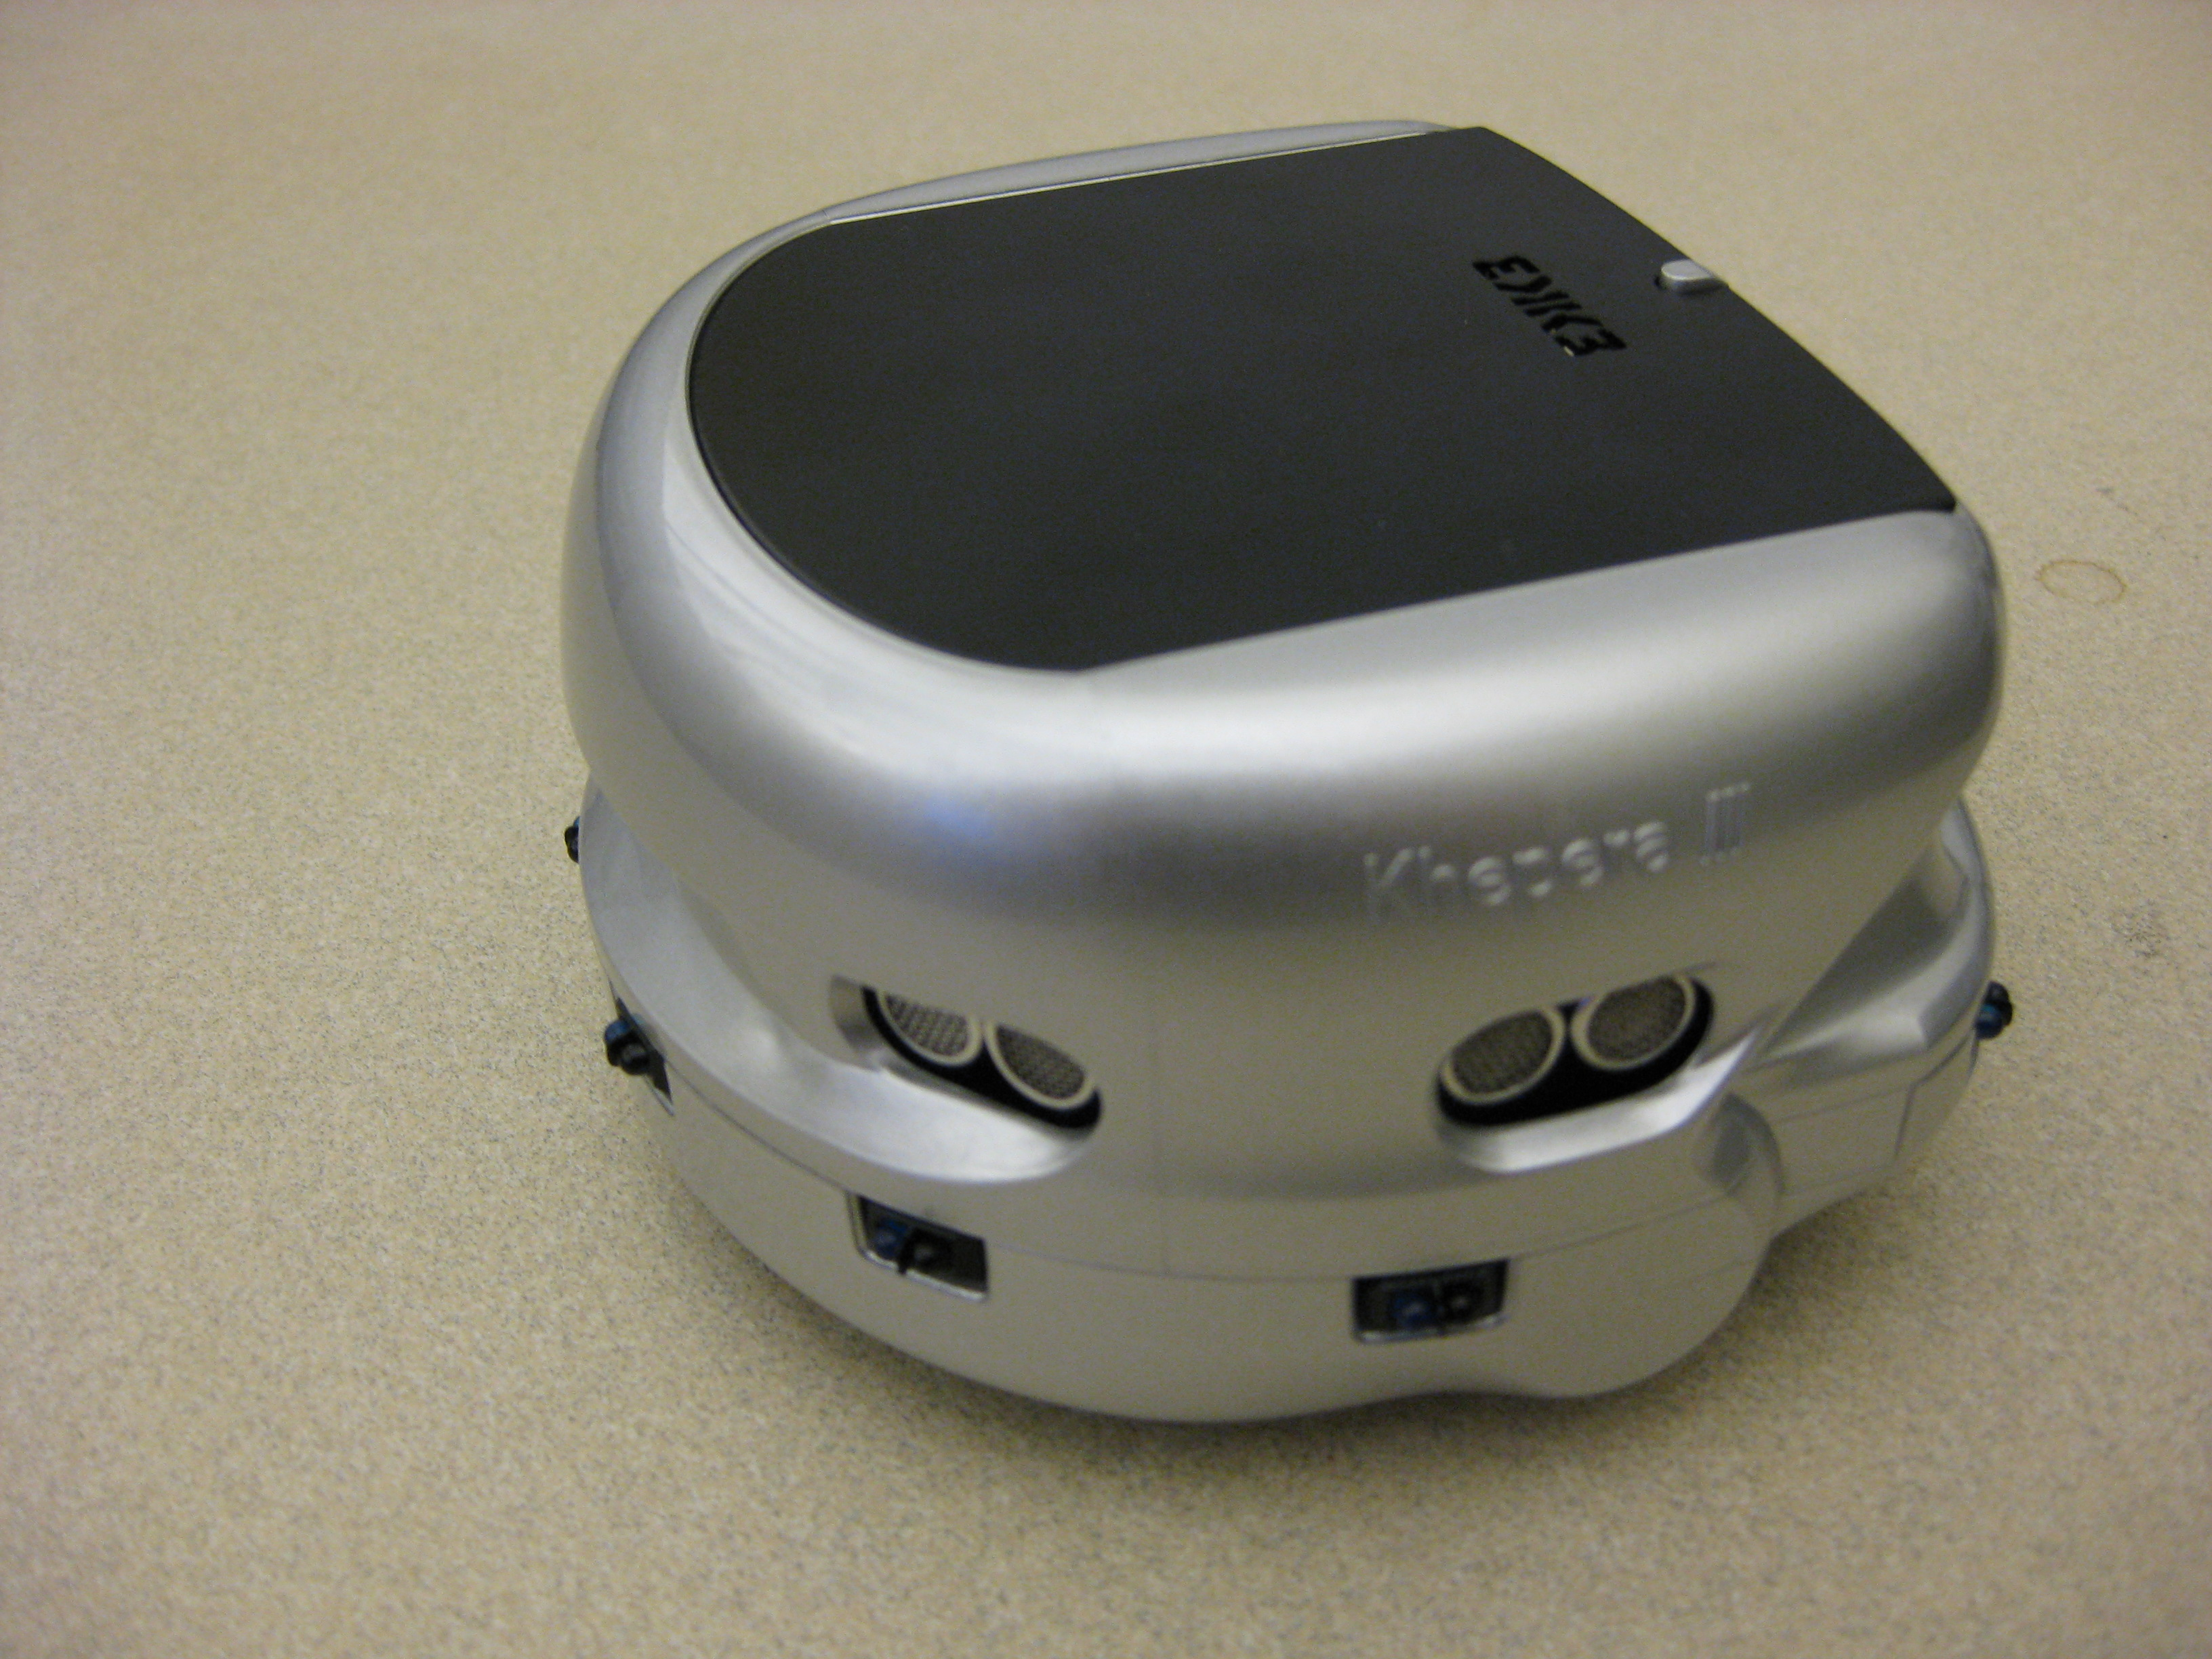
\includegraphics[trim= 8cm 0cm 0cm 0cm,clip,
scale=0.14]{Figuras/Khepera_III_robot}
		\subcaption{Robô Khepera 3}
	  	\label{fig:test1}
	\end{subfigure}
	~
	\begin{subfigure}[b]{0.49\textwidth}%
		\centering
		% fbox{}
		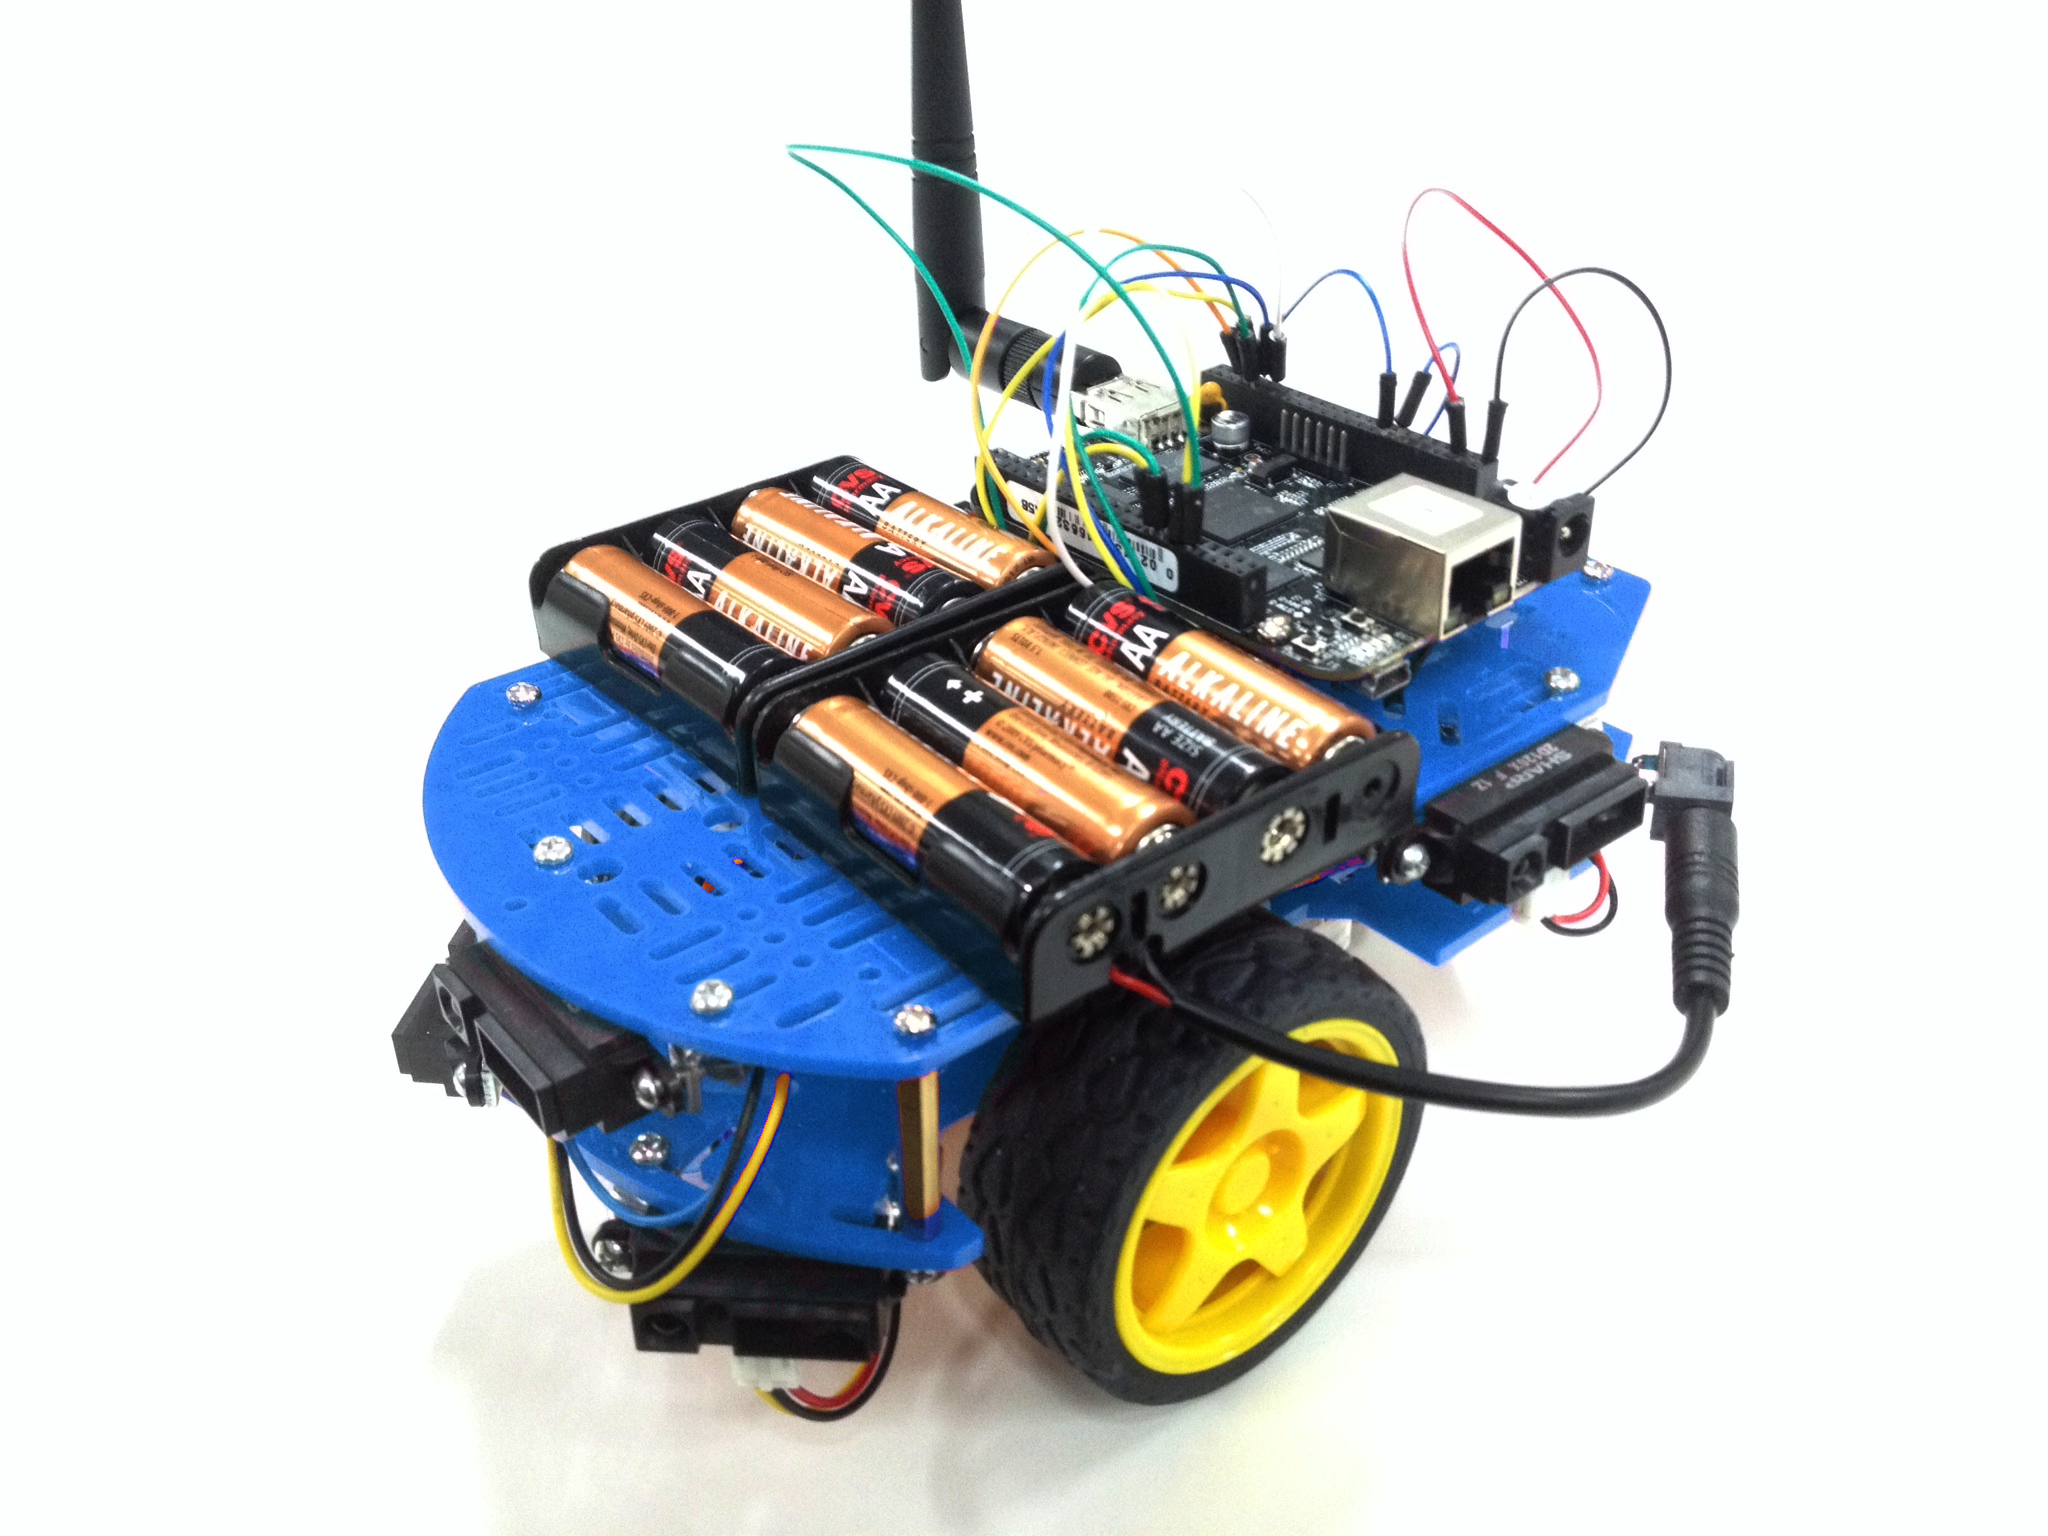
\includegraphics[trim={6cm 0cm 3cm 0cm},clip,
scale=0.09]{Figuras/quickbot-blue}
		\subcaption{Robô QuickBot}
	  	\label{fig:test2}
	\end{subfigure}
	
	\textbf{Fonte: \citeonline{im:Khepera}, \citeonline{im:QuickBot_Blue}}
\end{figure}


%		\begin{figure}[!htb]
%			\centering
%			\caption{Robôs Khepera e QuickBot fisicamente e em simulação}
%			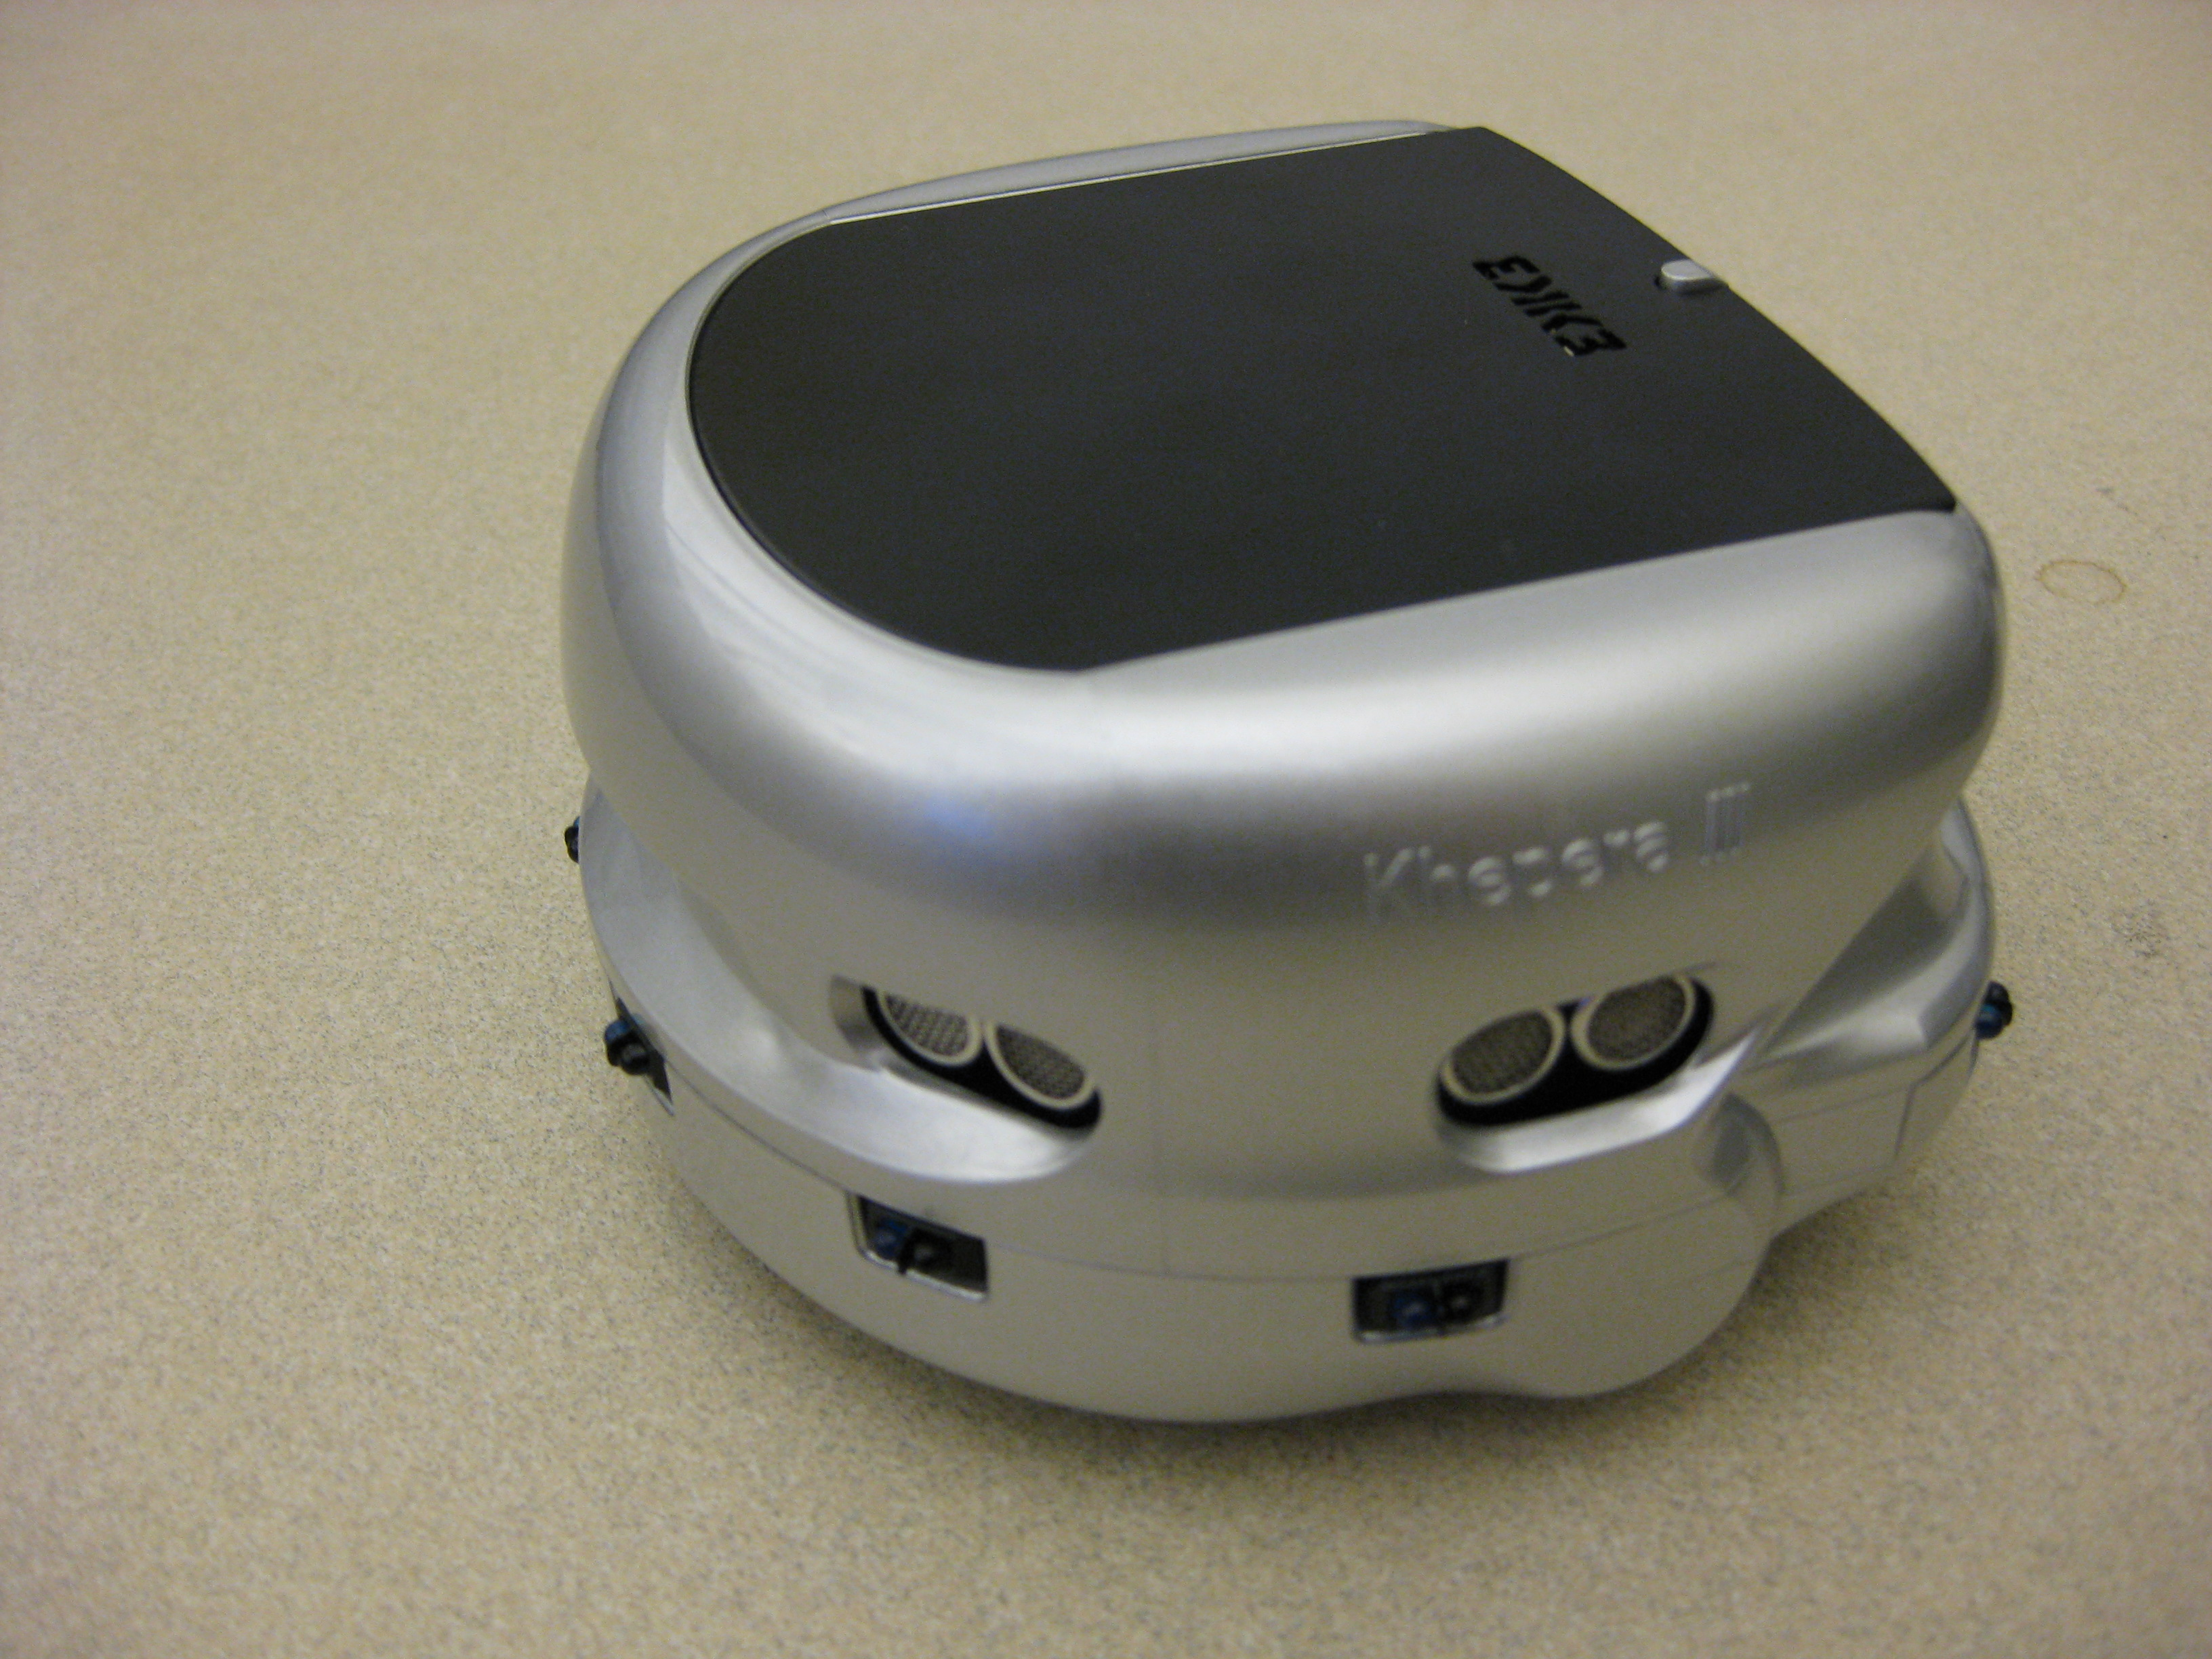
\includegraphics[trim={0cm 0cm 0cm 0cm},clip,
%scale=0.35]{Figuras/Khepera_III_robot}
%			%\vspace{-0.4cm}
%			\label{fig:RobosESim}
%		\end{figure}

%		\begin{figure}[!htb]
%			\centering			
%			\caption{Robôs Khepera e QuickBot fisicamente e em simulação}
%			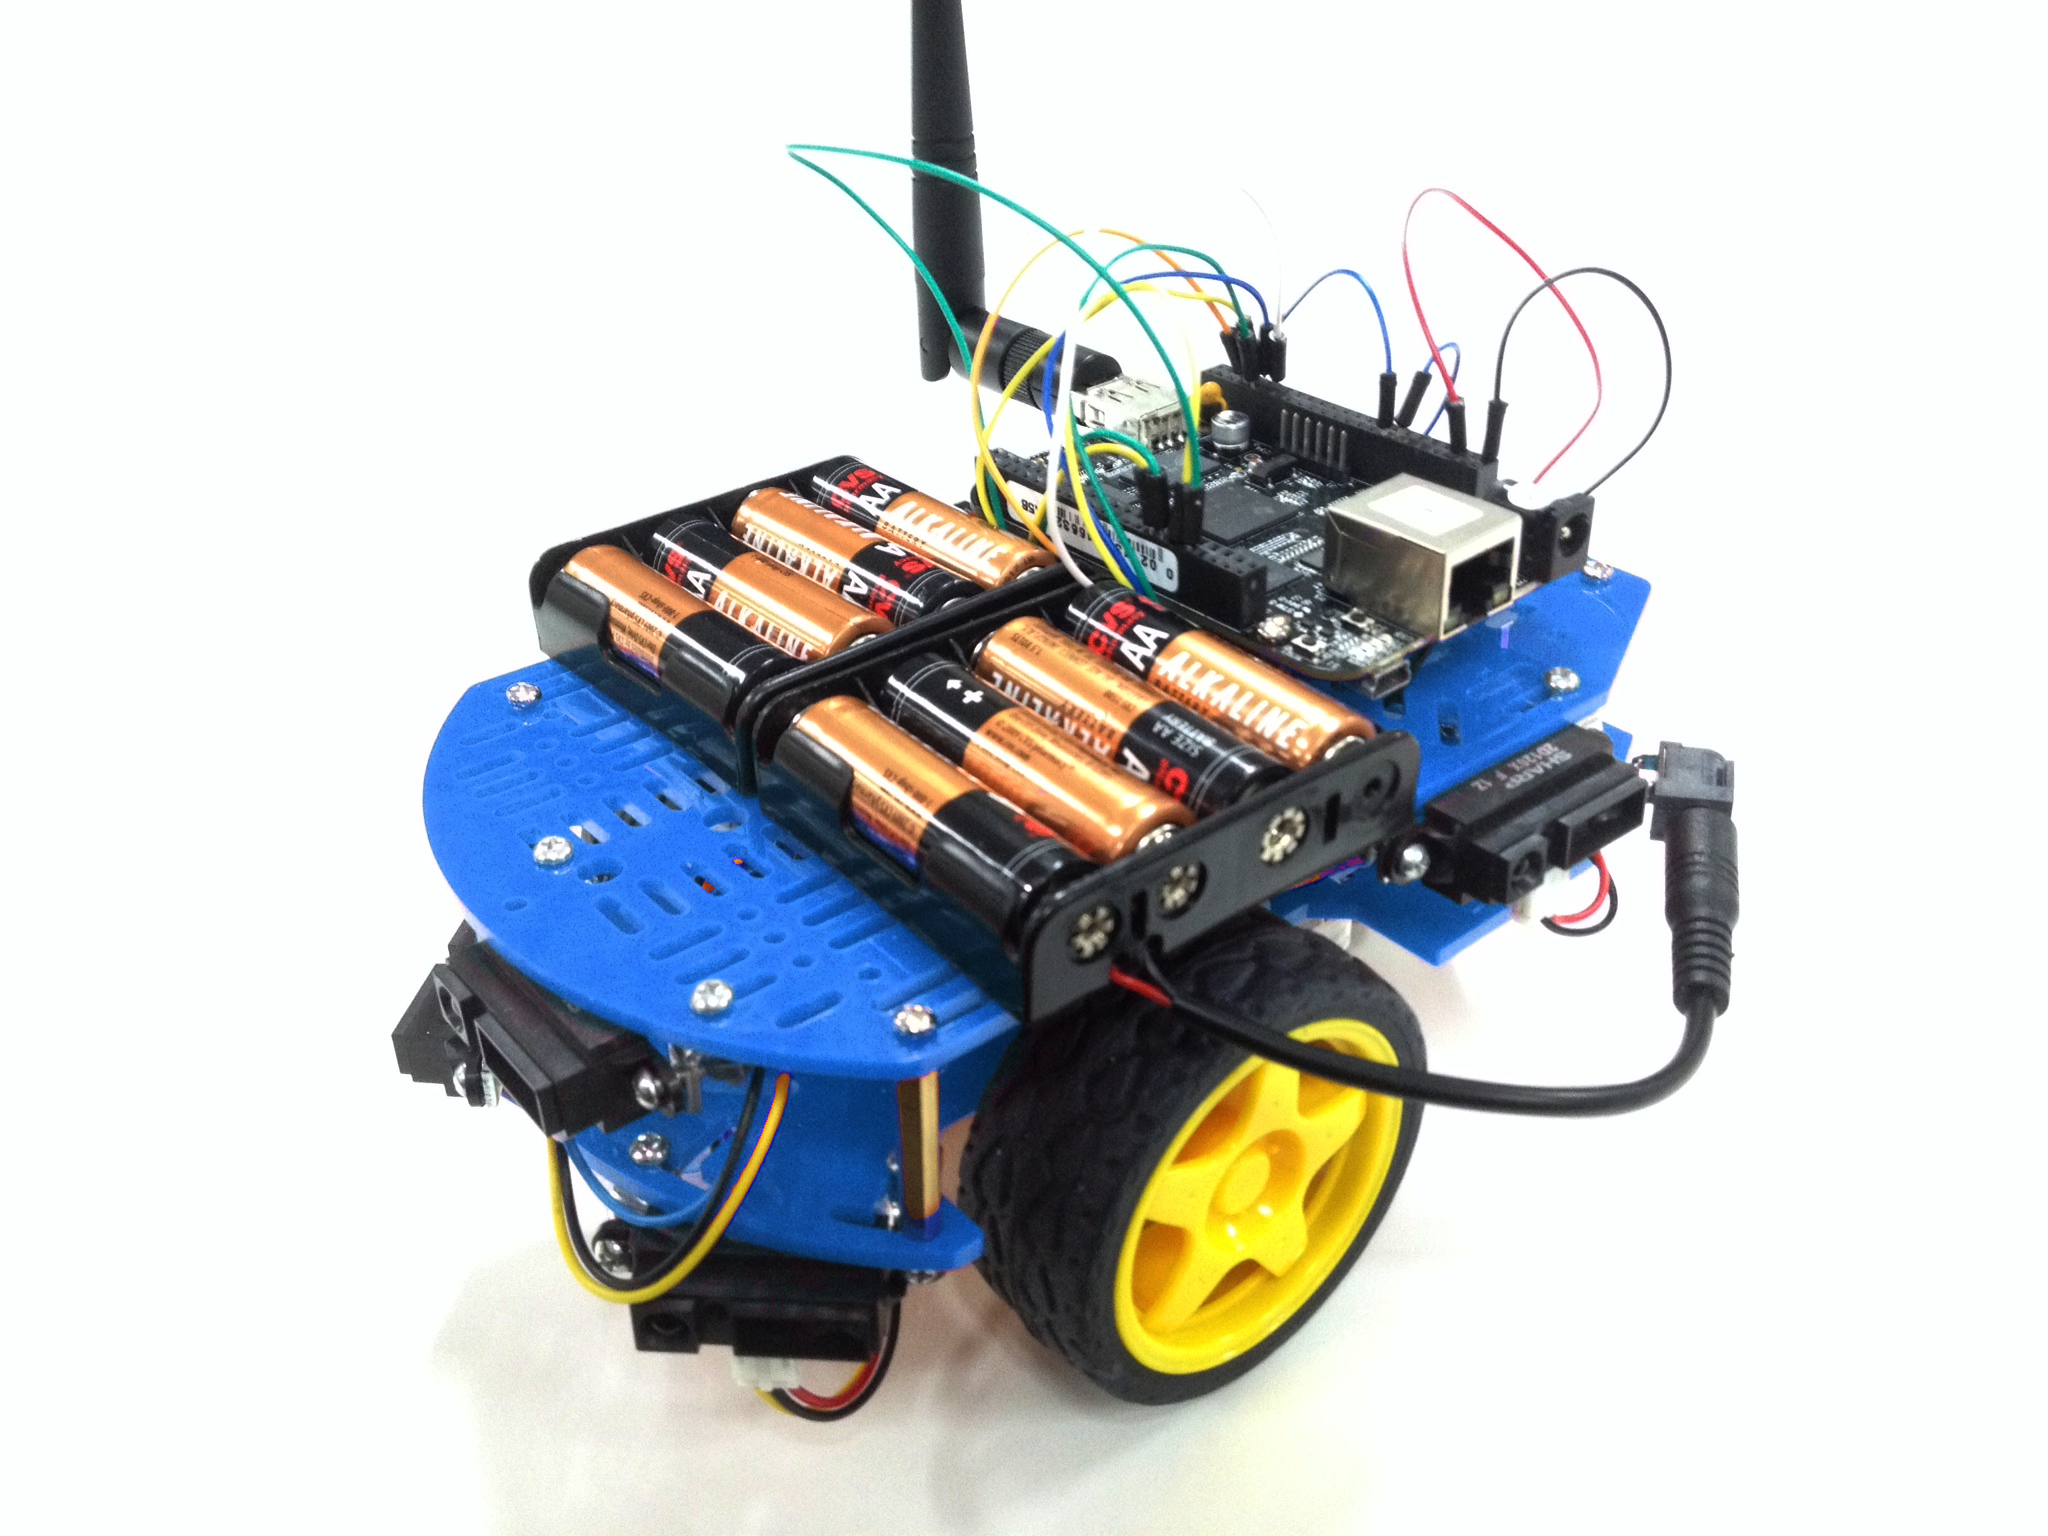
\includegraphics[trim={0cm 0cm 0cm 0cm},clip,
%scale=0.25]{Figuras/quickbot-blue}
%			%\vspace{-0.4cm}
%			\label{fig:RobosESim}
%		\end{figure}

%		\begin{figure}[!htb]
%			\centering
%			\caption{Robôs Khepera e QuickBot fisicamente e em simulação}
%			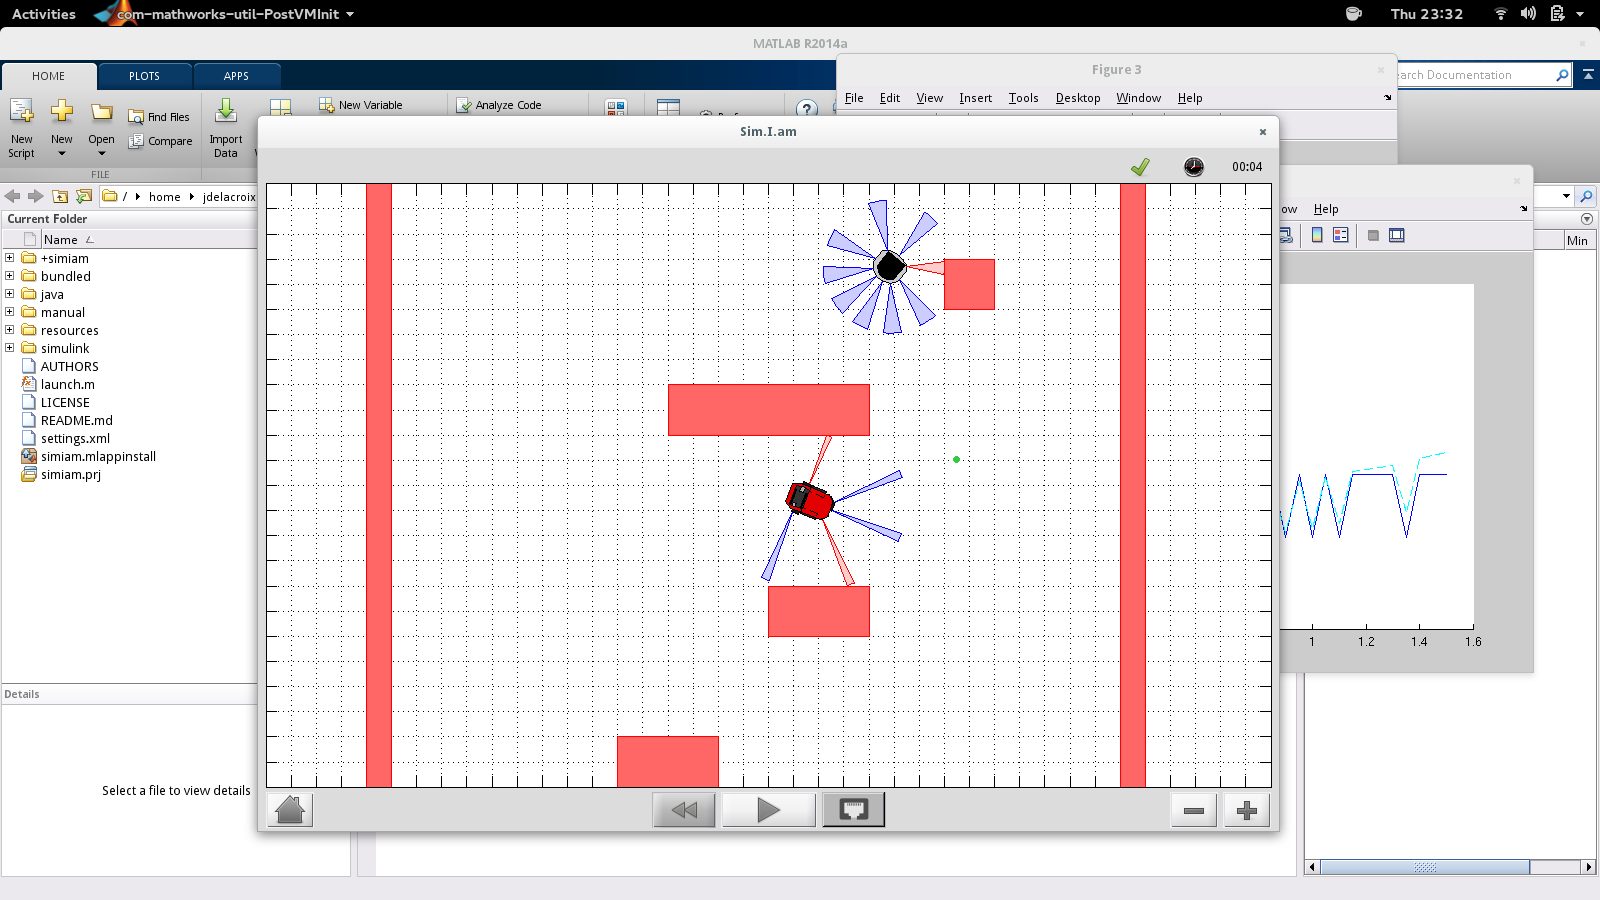
\includegraphics[trim={0cm 0cm 0cm 0cm},clip,
%scale=0.25]{Figuras/simiam-screenshot}
%			%\vspace{-0.4cm}
%			\label{fig:RobosESim}
%		\end{figure}


%\begin{figure}
%\begin{minipage}[c][11cm][t]{.5\textwidth}
%  \vspace*{\fill}
%  \centering
%  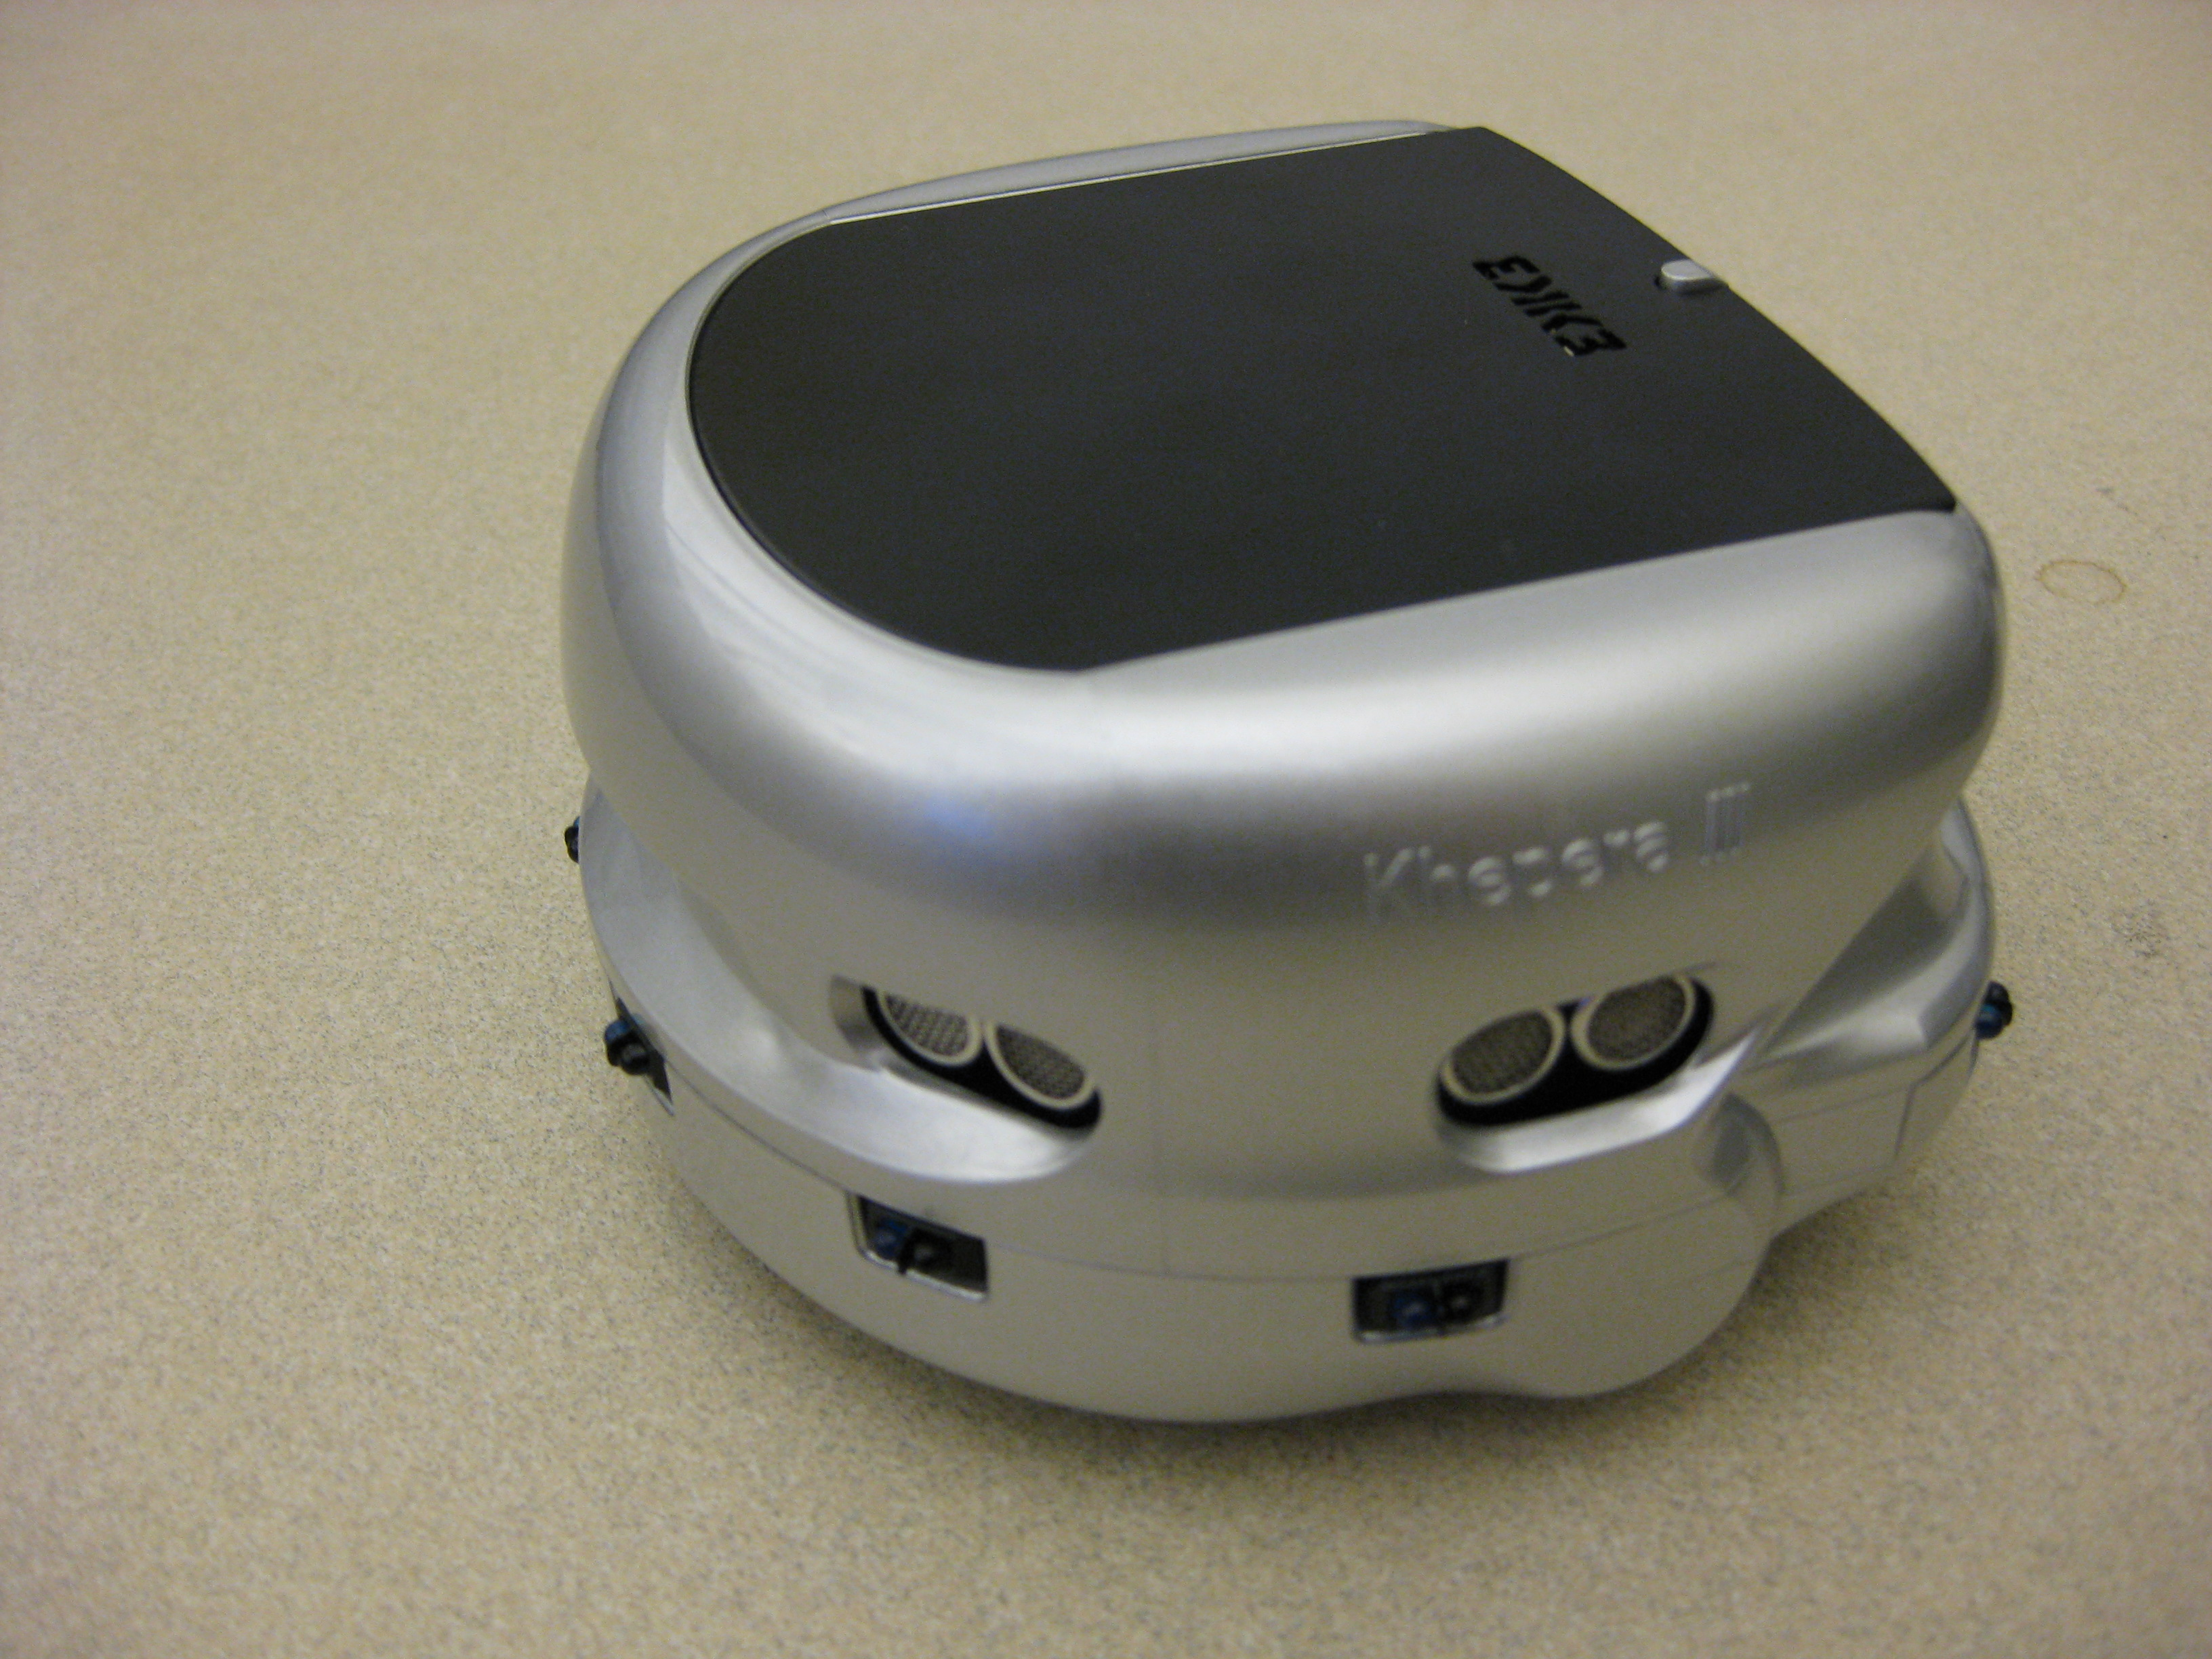
\includegraphics[width=5cm,height=4.5cm]{Figuras/Khepera_III_robot}
%  \subcaption{Robô Khepera}
%  \label{fig:test2}\par\vfill
%  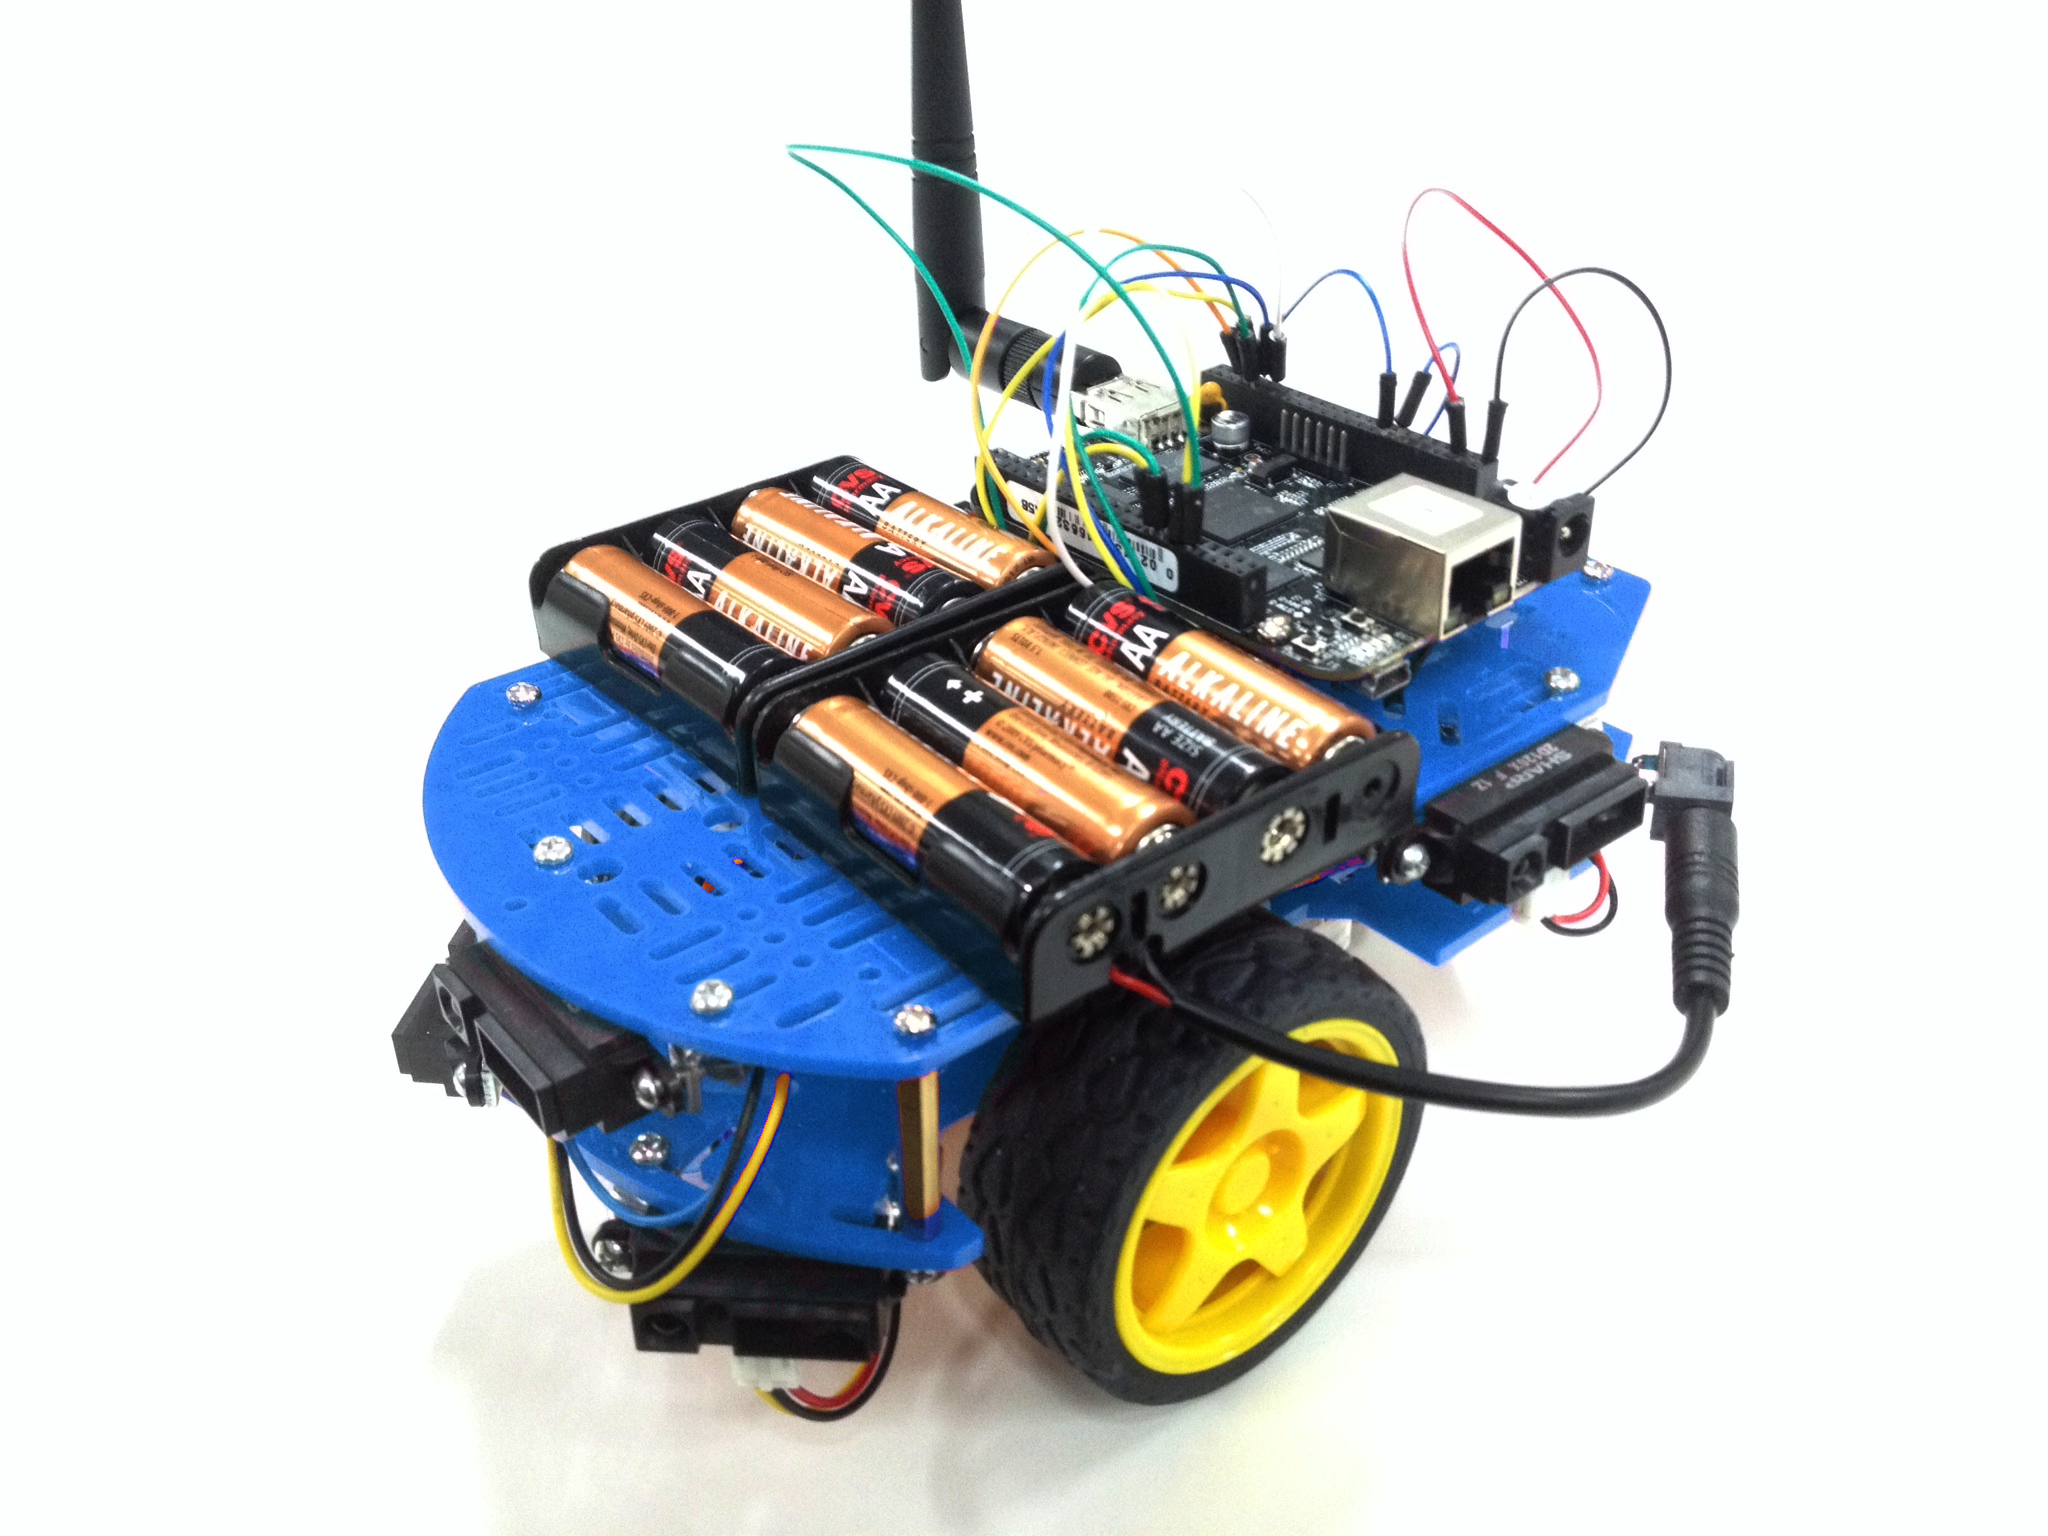
\includegraphics[width=5cm,height=4.5cm]{Figuras/quickbot-blue}
%  \subcaption{Robô QuickBot}
%  \label{fig:test3}
%\end{minipage}
%\begin{minipage}[c][11cm][t]{.5\textwidth}
%  \vspace*{\fill}
%  \centering
%  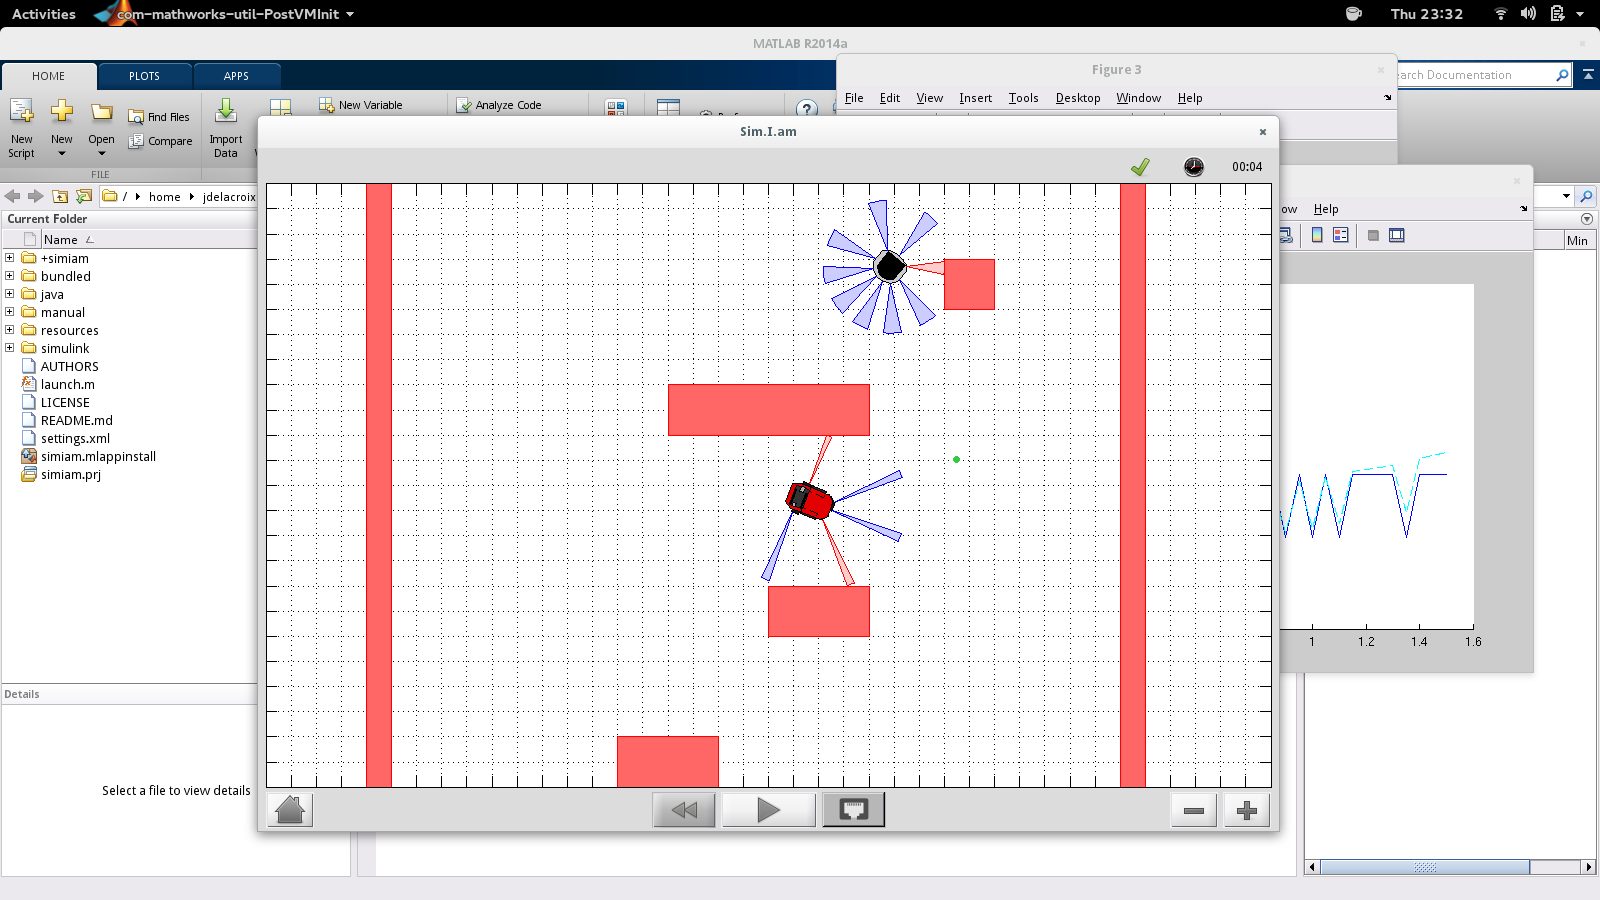
\includegraphics[width=5cm,height=10cm]{Figuras/simiam-screenshot}
%  \subcaption{Simulador Simiam}
%  \label{fig:test1}
%\end{minipage}%
%\end{figure}
	\onslide<3>
	\vspace{-3.5cm}
	\begin{figure}[h]
\centering
%\caption{Robôs Khepera 3 e QuickBot em simulação}
\label{fig:RobosEmSimulador}
		\centering
		% fbox{}
		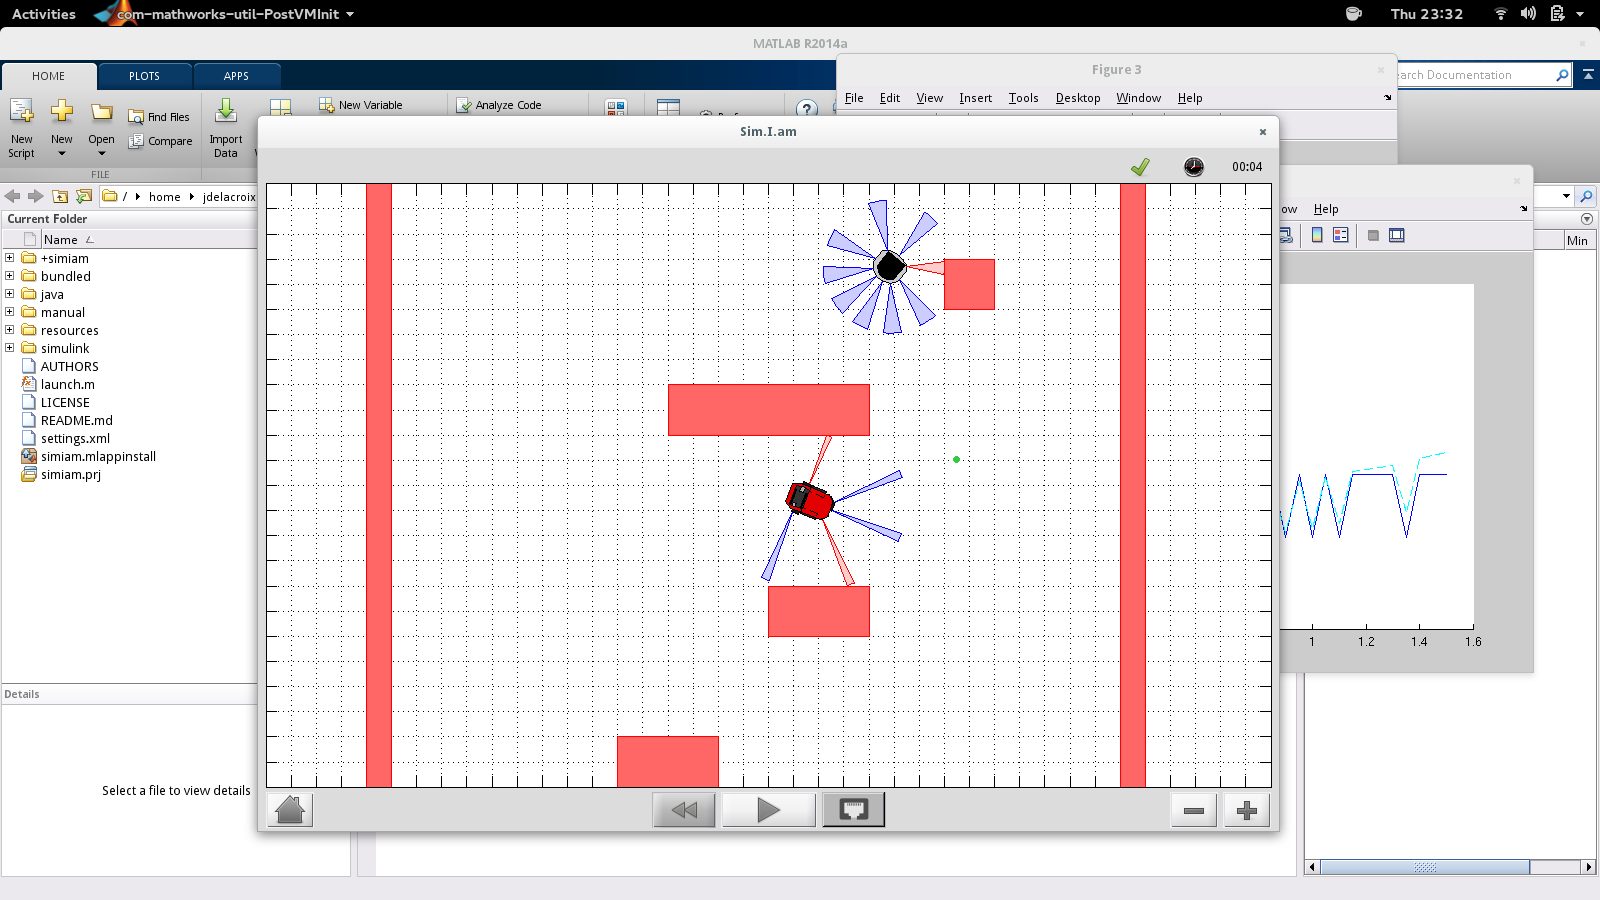
\includegraphics[trim={0cm 0cm 0cm 0cm},clip,
scale=0.16]{Figuras/simiam-screenshot}
	
	%\textbf{Fonte: \citeonline{im:Simiam}}
\end{figure}
\end{frame}

\begin{frame}
	\frametitle{Especificações}
	\begin{figure}[h]
	\centering
	\caption{Resposta do sensor infravermelho}
	\label{fig:SensorIR}
	
	%\fbox{}
	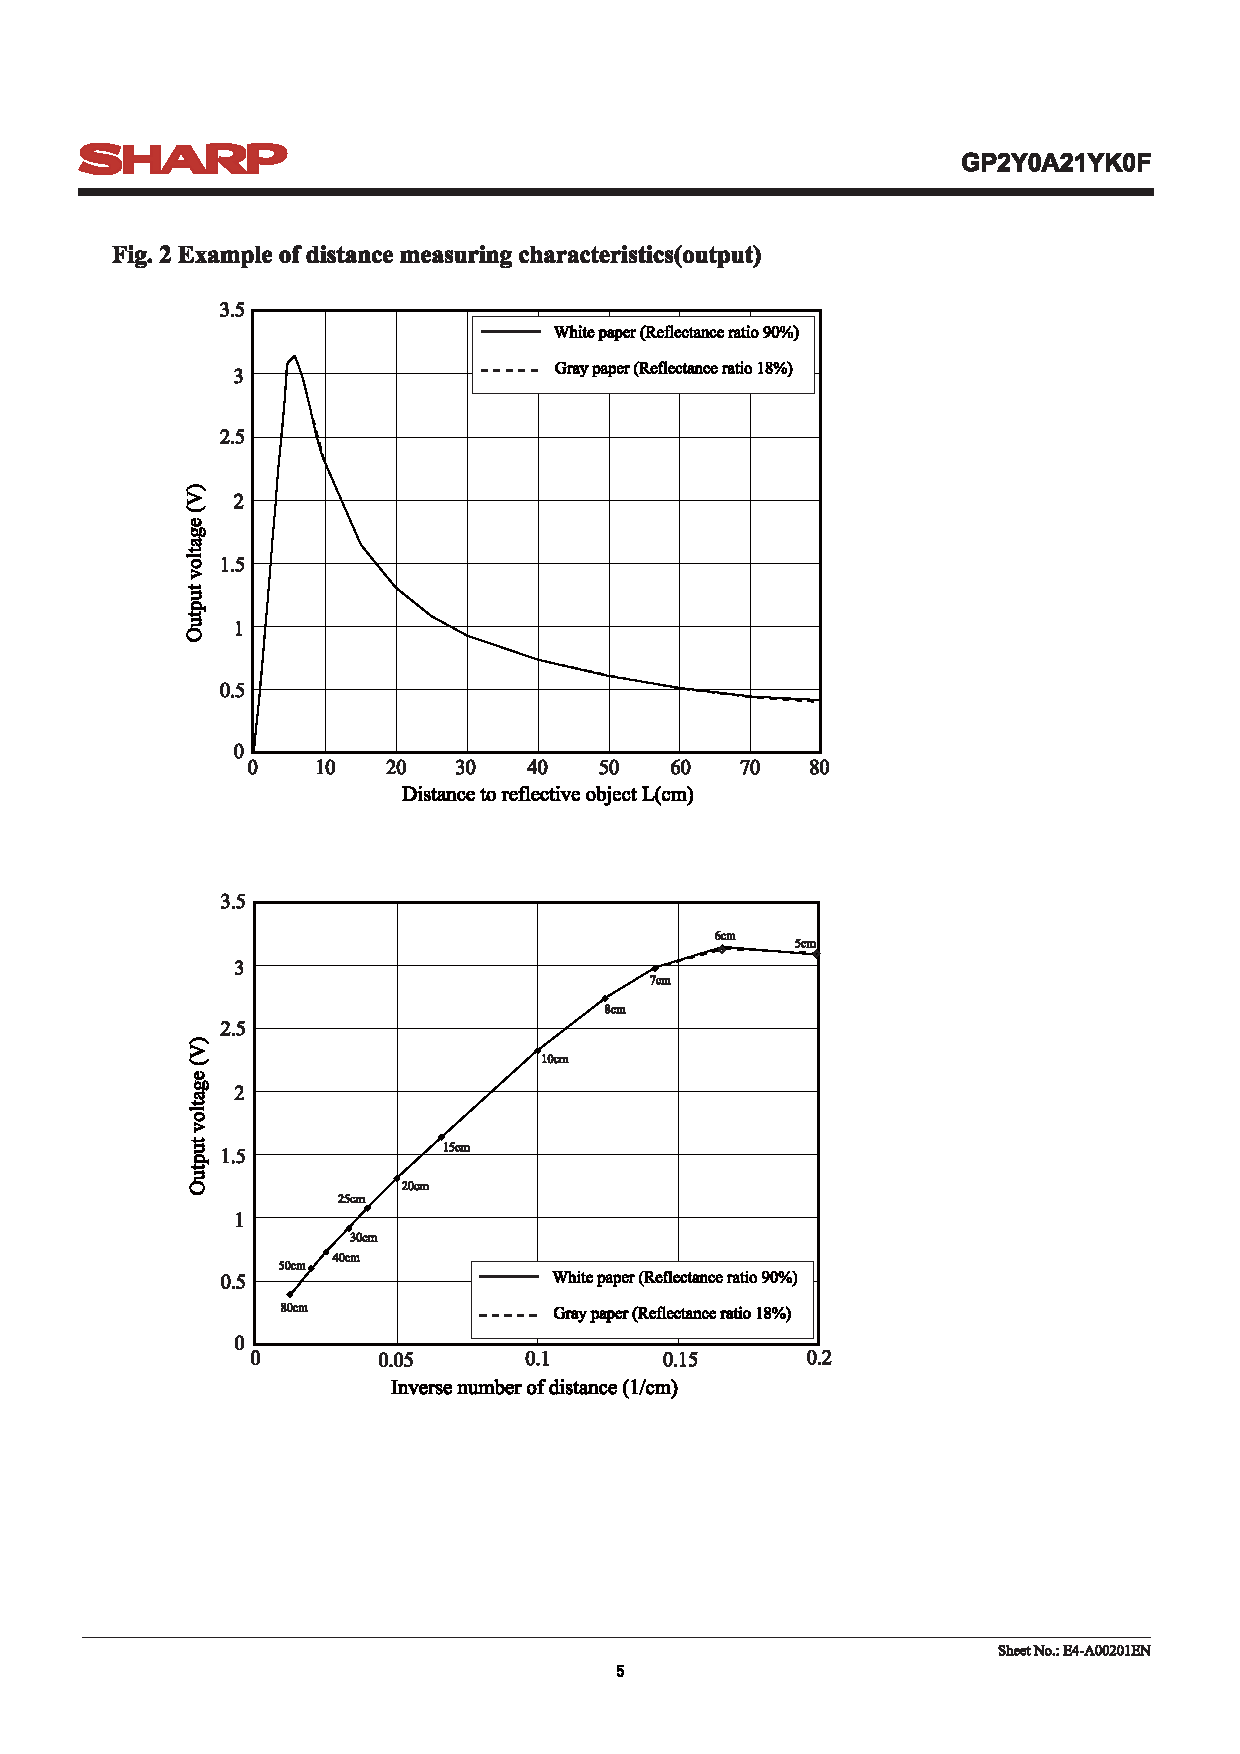
\includegraphics[trim= 3cm 15.8cm 6.5cm 4.8cm,clip,
scale=1]{Figuras/IR_Datasheet_Figure}

	%\begin{tikzpicture}[auto, node distance=2cm, on grid,
%>=latex']%
	
	%\node[anchor=south west,inner sep=0] (image) at (0,0) {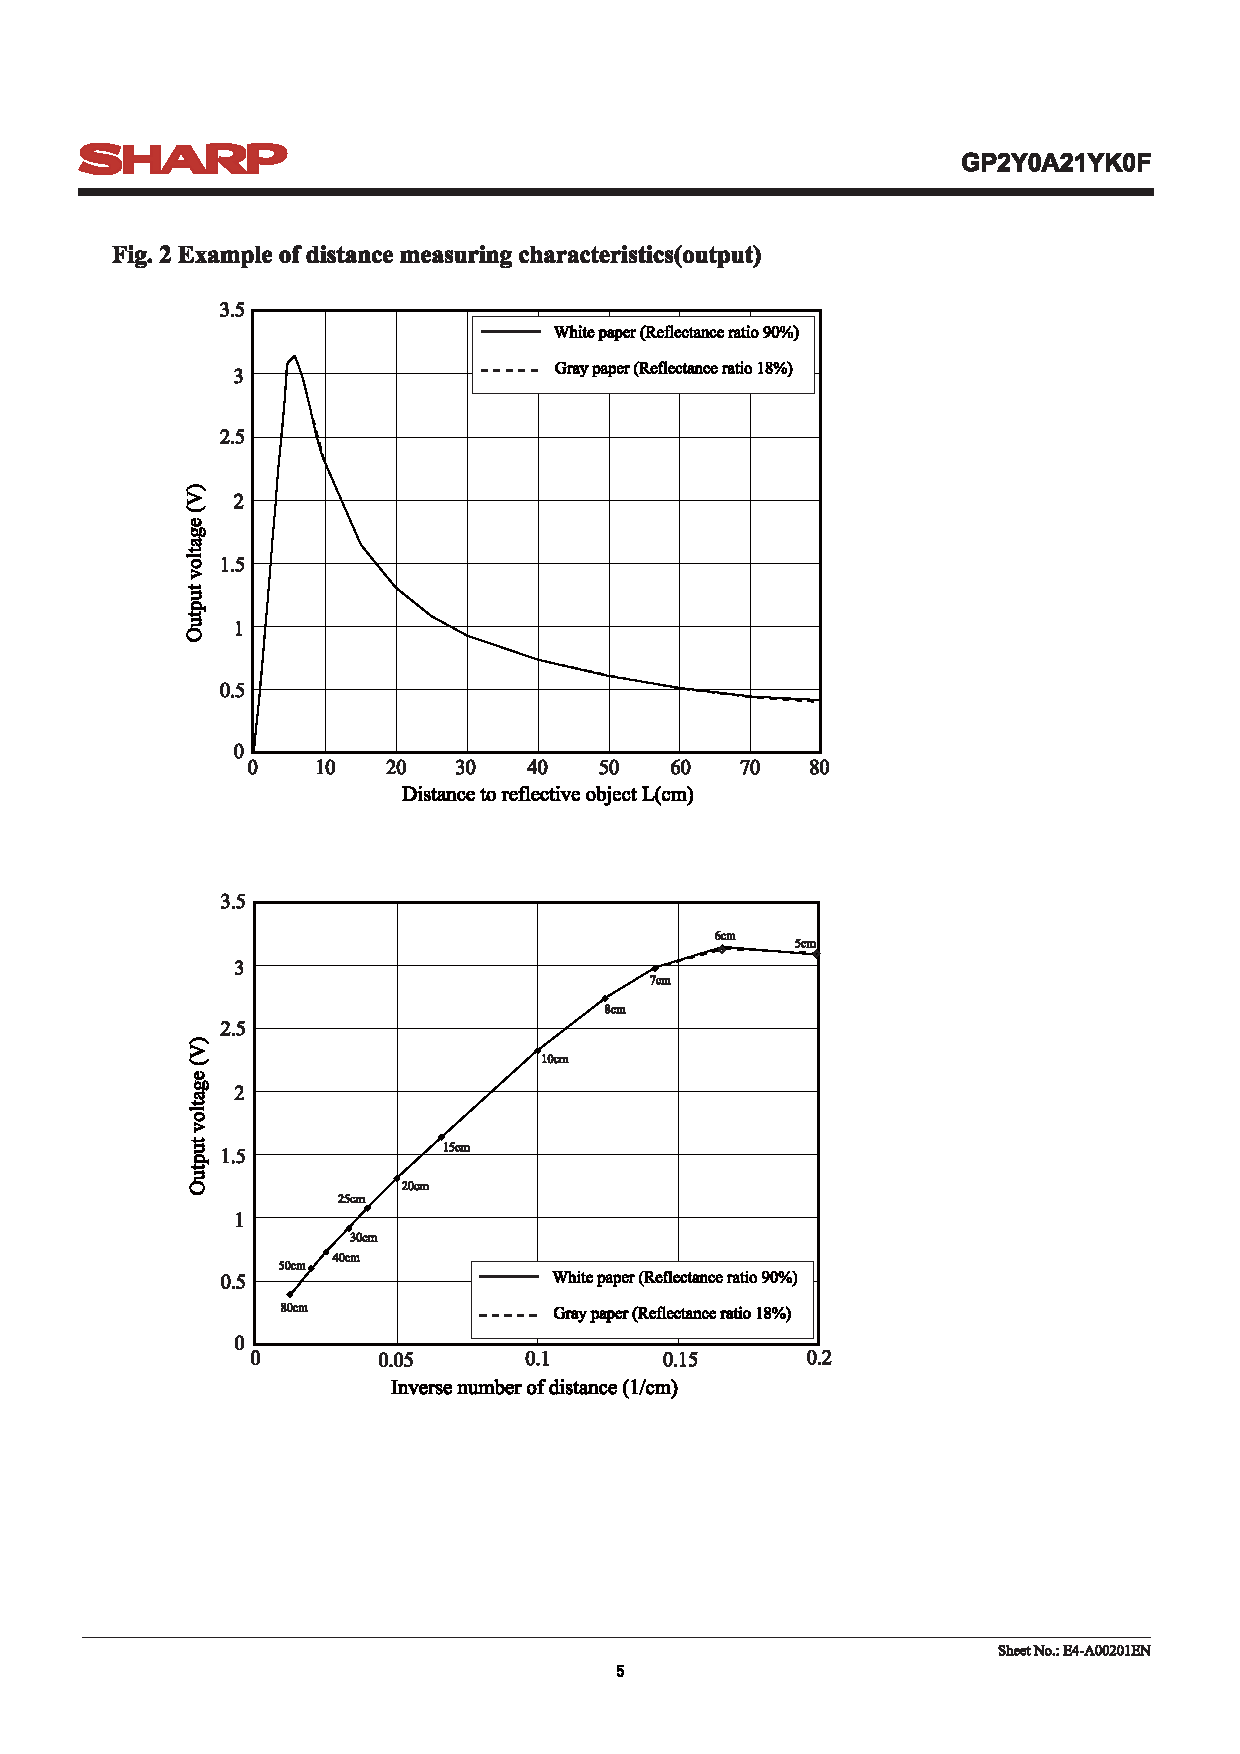
\includegraphics[trim =
%		{3cm 15.8cm 6.5cm 4.8cm}, clip,scale=1]{Figuras/IR_Datasheet_Figure}};
		
%	\node[fill,circle,inner sep=0.1pt, color = red] at (1.29,1.161) {};
%	\node[fill,circle,inner sep=0.1pt, color = red] at (2.525,2.235) {};
	
%	\node[fill,circle,inner sep=0.1pt, color = red] at (1.83,7.75) {};
	
	
%	\node[inner sep = 0 pt, outer sep = 0 pt] (origin) at (1.3,1.15) {};
%	\node[inner sep = 0 pt, outer sep = 0 pt] (teste2) at (2.55,2.25) {};
%	
%	\node[inner sep = 0 pt, outer sep = 0 pt] (P1) at (1.85,7.85) {};
	
	%\draw[-, color = red] (origin) -- (teste2);
	%\draw[-, color = red] (origin) -- (P1);
	
	%\node[] at (0,0) {};
	%\coordinate[] (teste1) {};
	%\coordinate[] (teste2) {};
	
	%\draw[-, color = red] (-18,2) -- (-7,3);
	
%	\end{tikzpicture}


	\textbf{Fonte: \citeonline{datasheet:SensorIR}}
\end{figure}
	\onslide<2>
		\begin{exampleblock}{Parâmetros}
			\begin{itemize}
			  \item Sensor IR: intervalo entre 10 e 80cm.
			  \item L = 18cm.
			  \item R = 3.4cm.
			\end{itemize}	
		\end{exampleblock}	
	\onslide<3>
		\vspace{-3.2cm}
		\begin{exampleblock}{Equação para distâncias do sensor IR}
			\begin{equation}
				\begin{split}
					d(v) = 2.7802212625 v^6 -35.1150300110 v^5 + 179.6031433005 v^4 \\
					-477.9449116299 v^3 + 706.3400747125 v^2 -569.7367375002 v \\
					+ 221.2678651473
				\end{split}
			\end{equation}
		\end{exampleblock}
\end{frame}

\begin{frame}
	\frametitle{Montagem Física}
	\begin{figure}[h]
\centering
\caption{Materiais e robô após montagem}
\label{fig:RoboReal}
	\begin{subfigure}[b]{0.49\textwidth}%
		\centering
		% fbox{}
		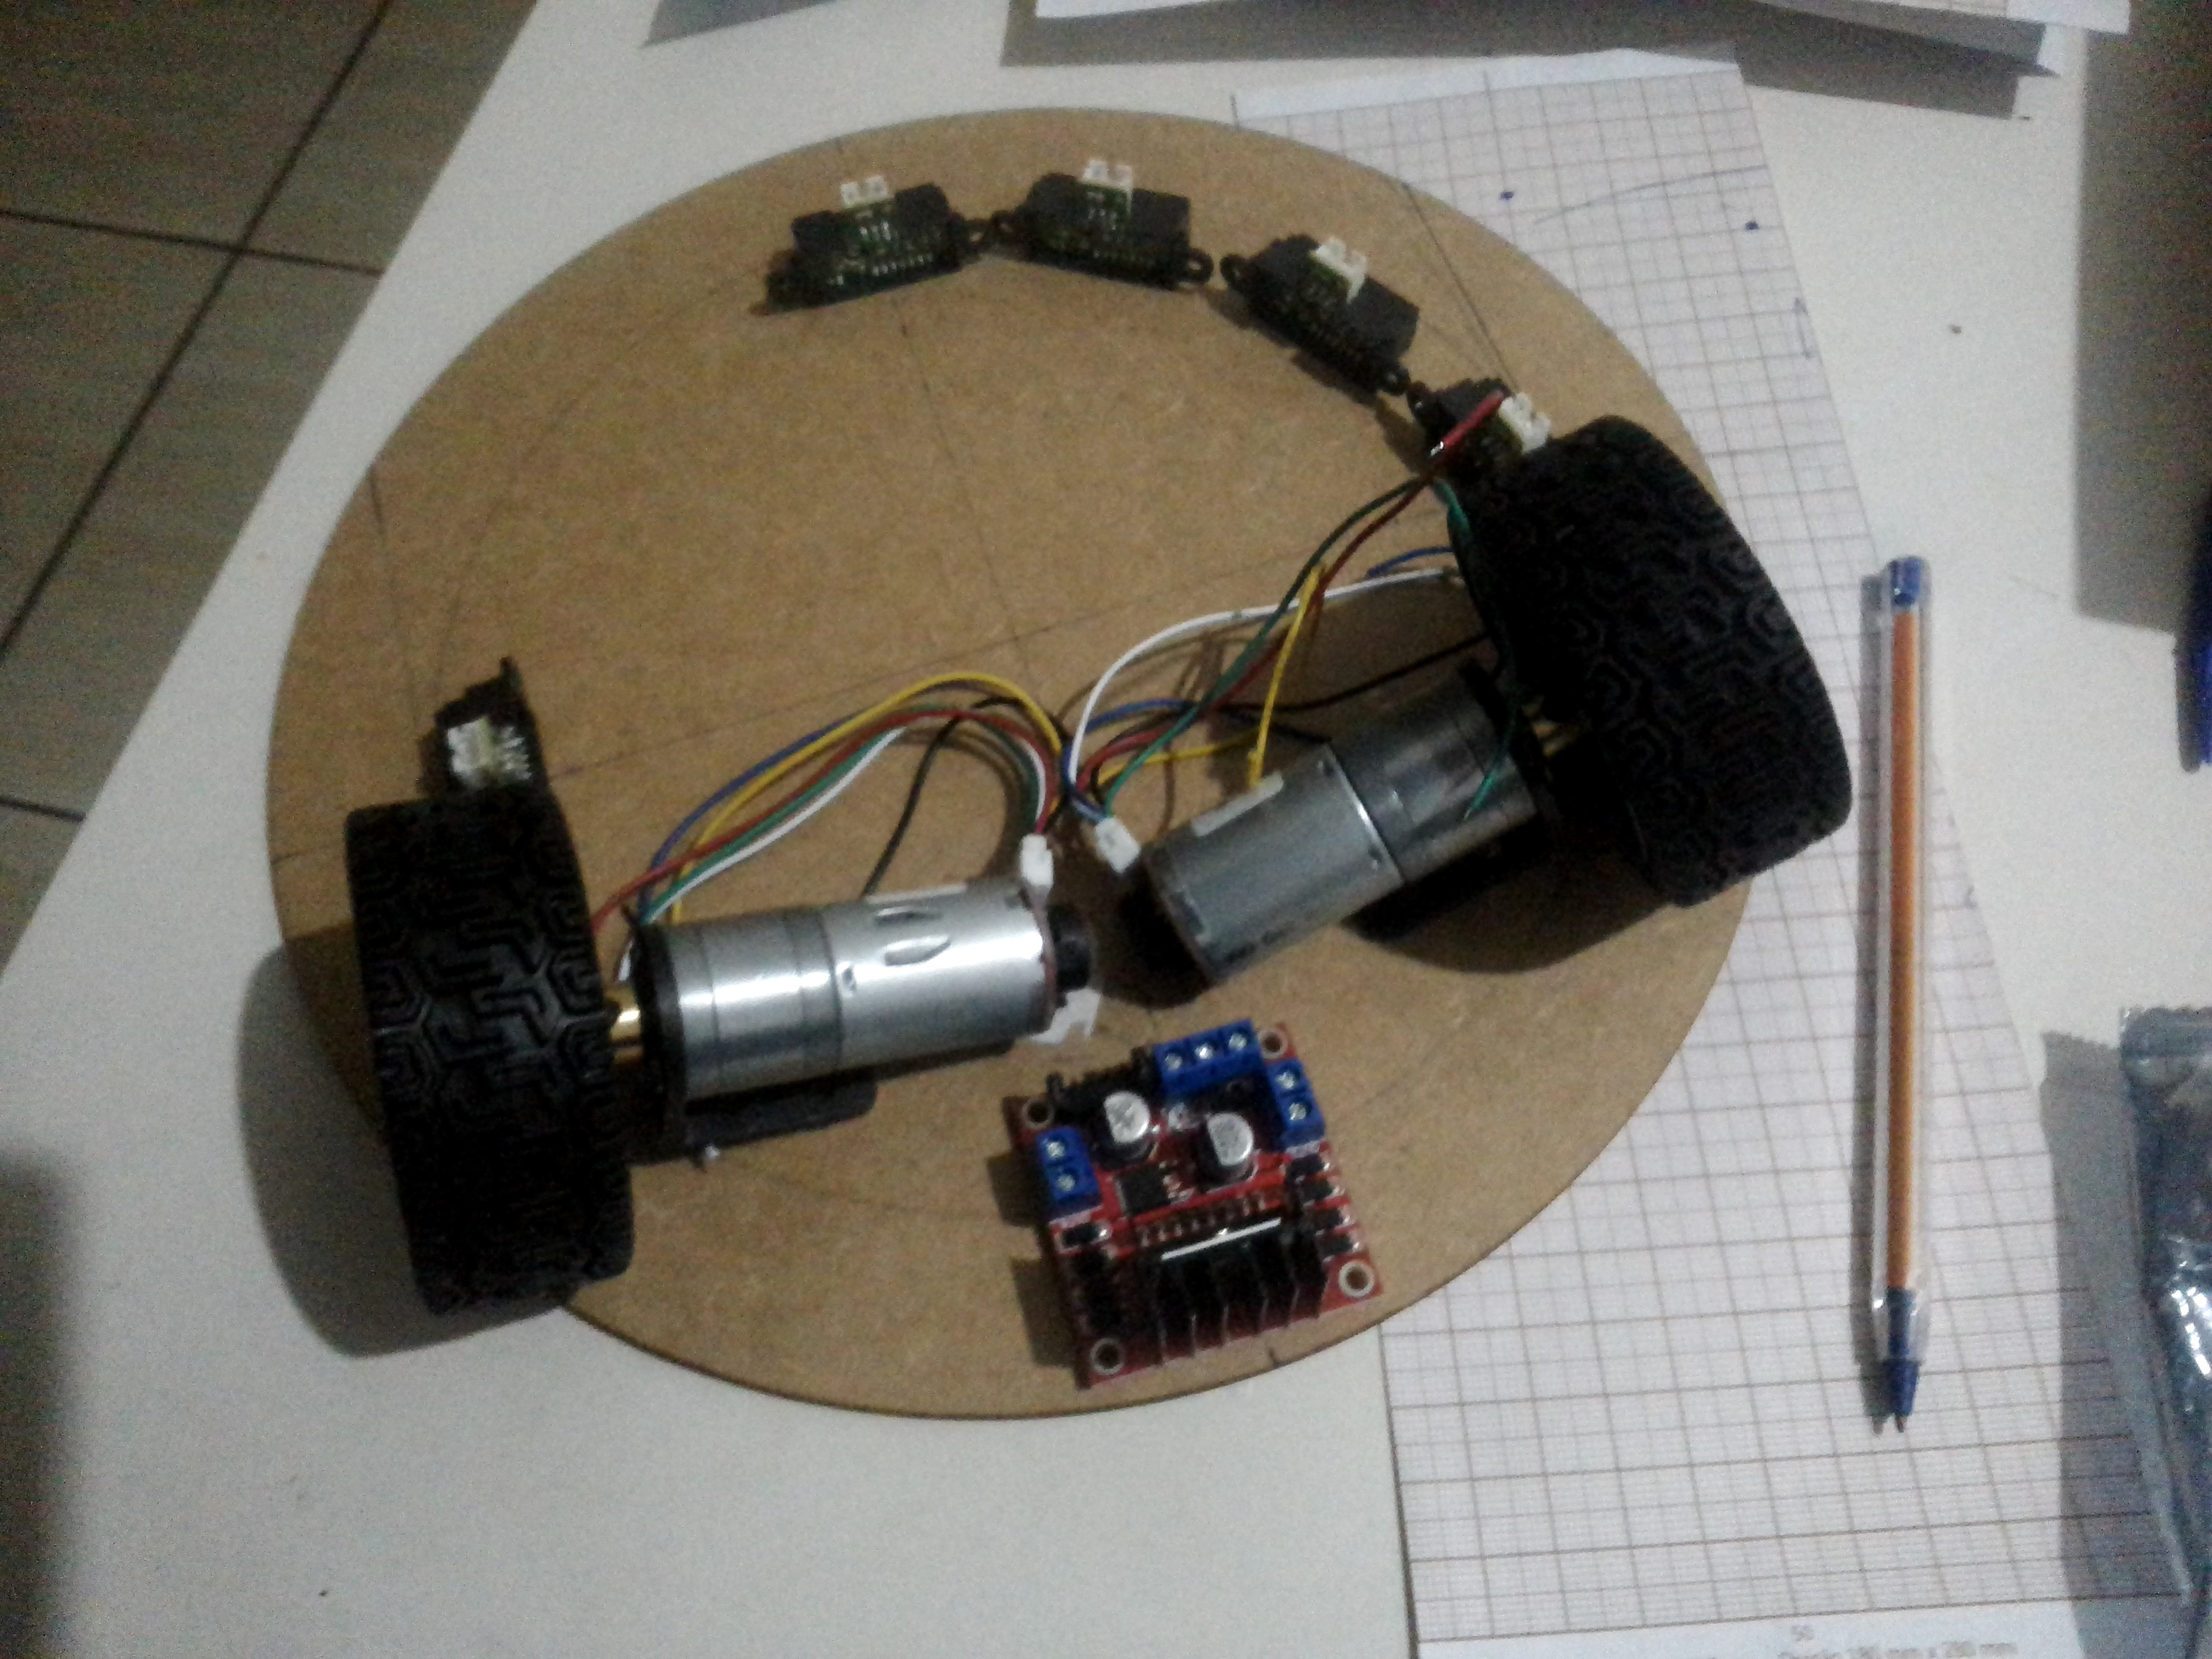
\includegraphics[trim= 0cm 0cm 0cm 0cm,clip,
scale=0.07]{Figuras/Robo1}
		\subcaption{Materiais do robô}
	  	%\label{fig:test1}
	\end{subfigure}
	~
	\begin{subfigure}[b]{0.49\textwidth}%
		\centering
		% fbox{}
		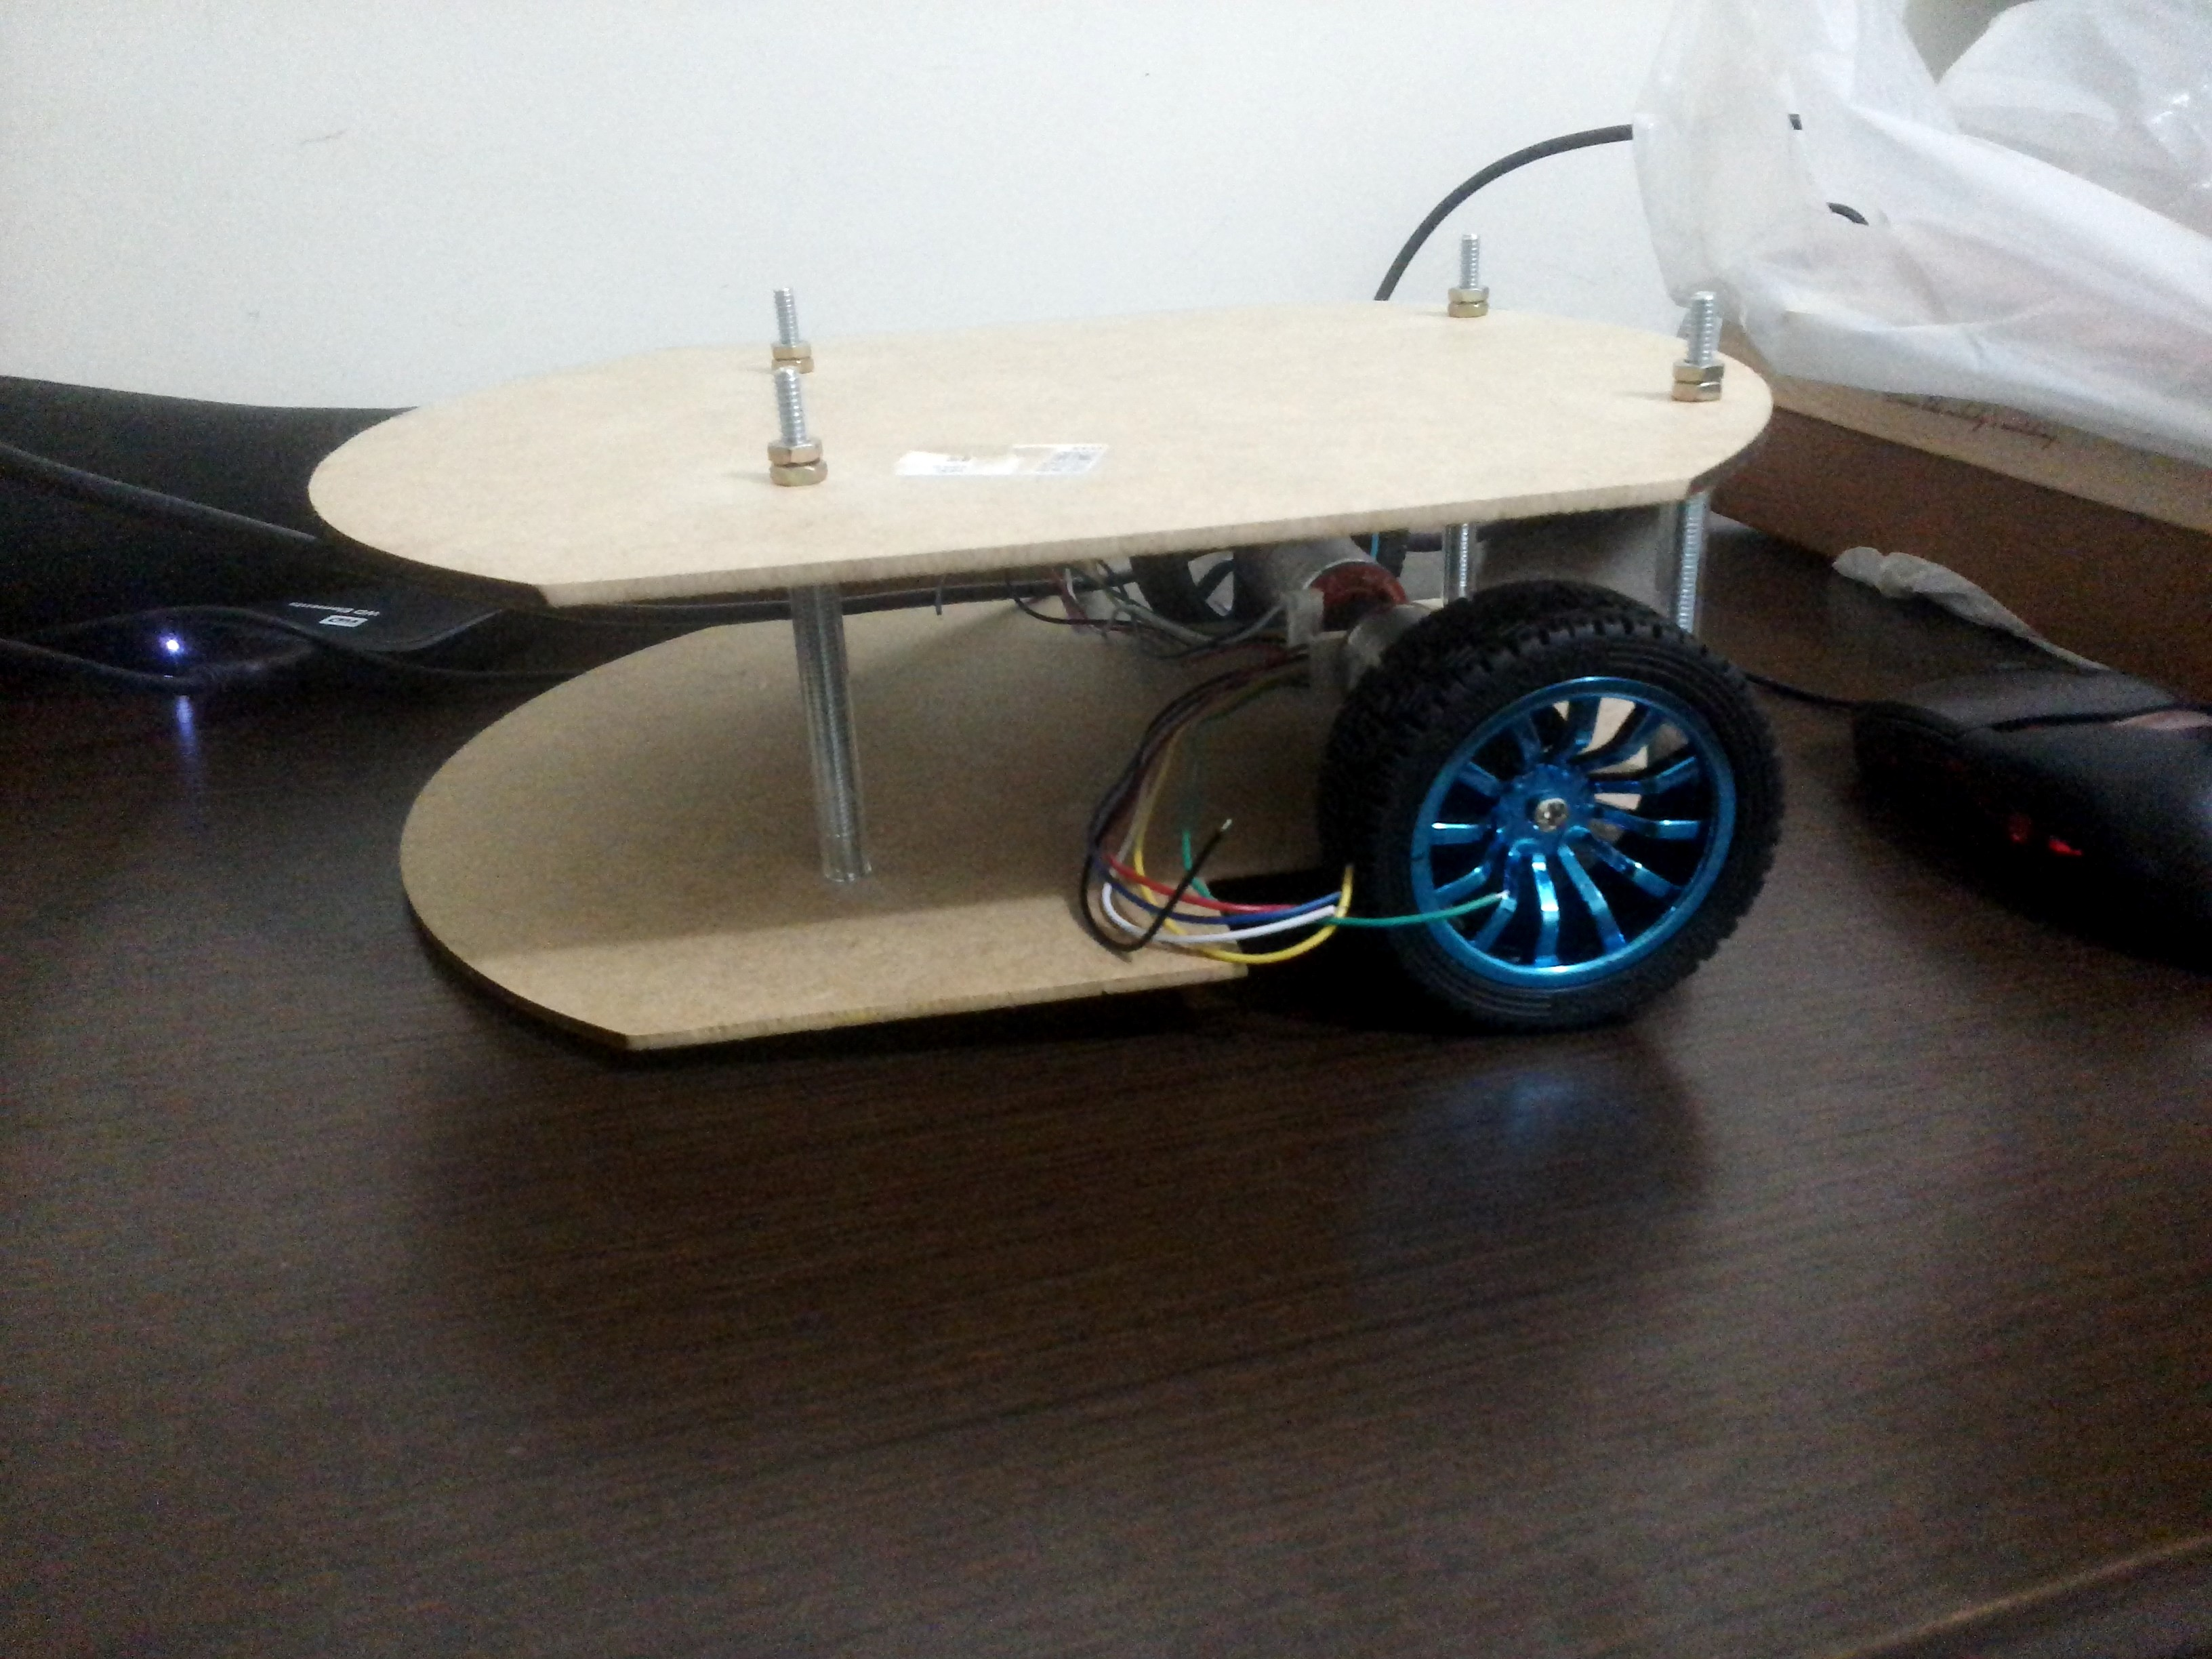
\includegraphics[trim={0cm 0cm 0cm 0cm},clip,
scale=0.07]{Figuras/Robo2}
		\subcaption{Robô montado}
	  	%\label{fig:test2}
	\end{subfigure}
	
	\textbf{Fonte: autoria própria}
\end{figure}
\end{frame}

\begin{frame}
	\begin{figure}[!ht]
\centering
	\begin{subfigure}[b]{0.49\textwidth}%
		\centering
		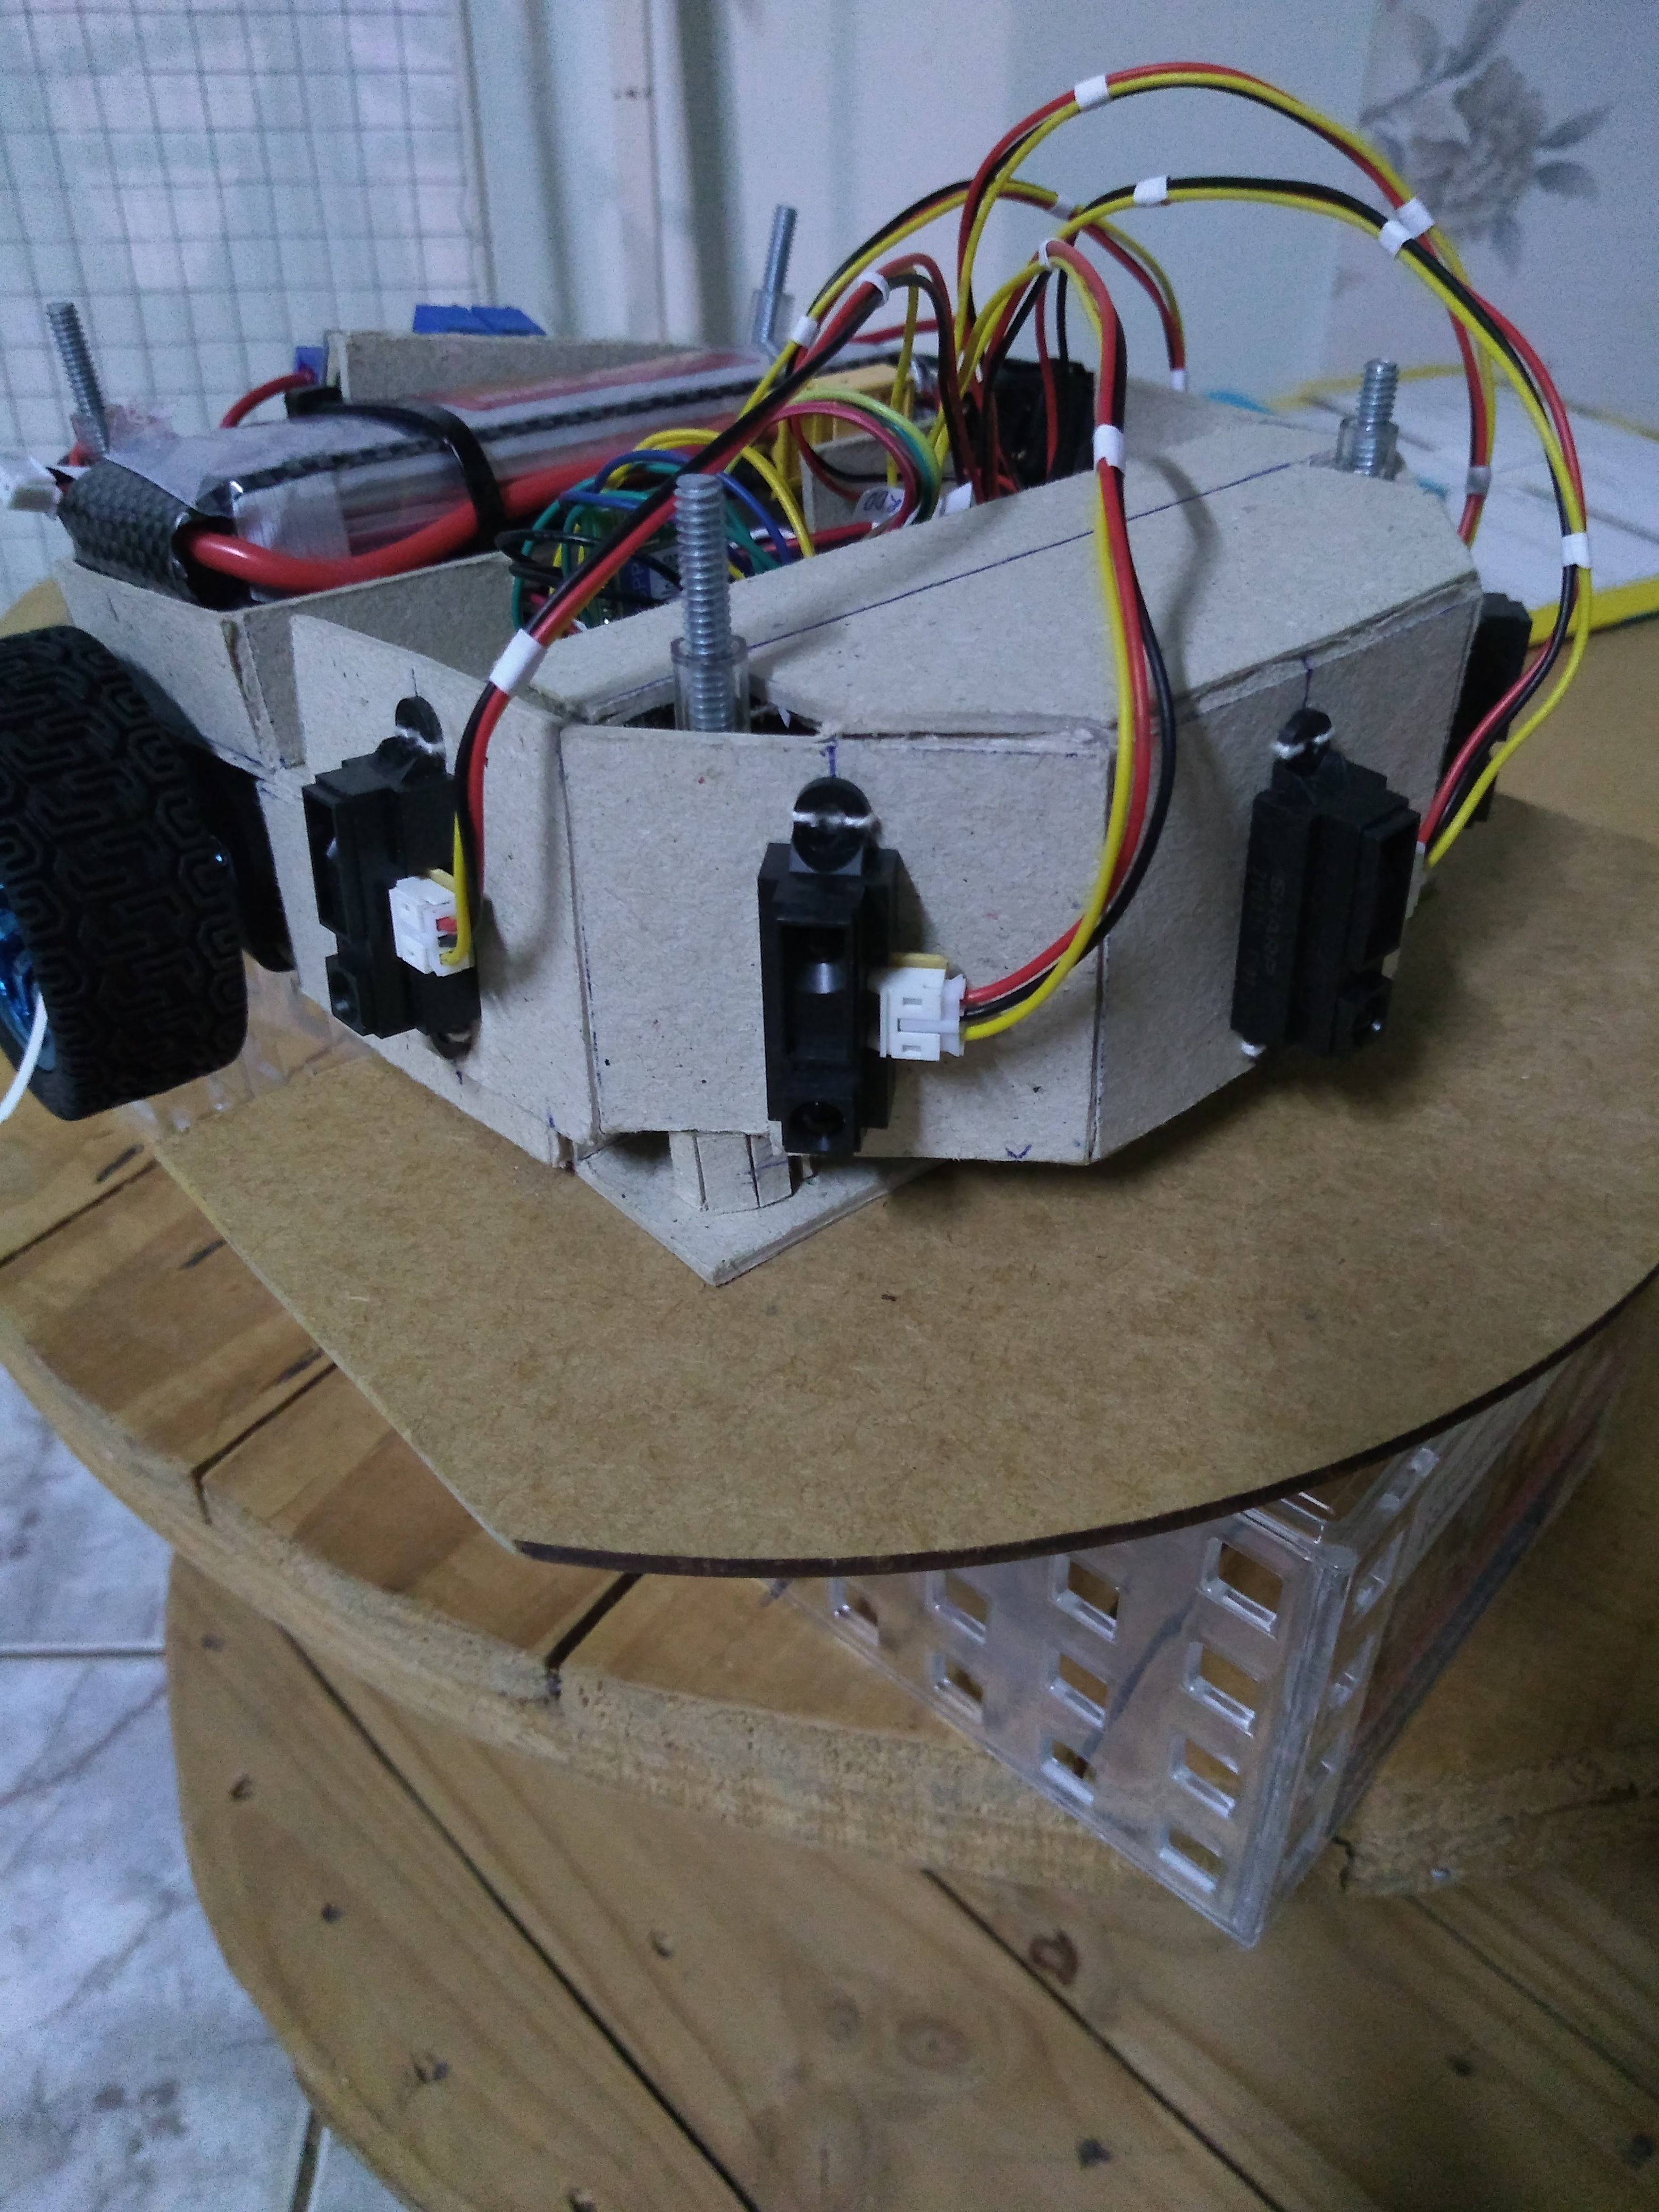
\includegraphics[trim={0cm 35cm 0cm 0cm}, clip, 
		scale=0.055]{Figuras/RoboMontagem5}%
		\subcaption{Posição dos parafusos de rosca}%
	\end{subfigure}%
	~
	\begin{subfigure}[b]{0.49\textwidth}%
		\centering
		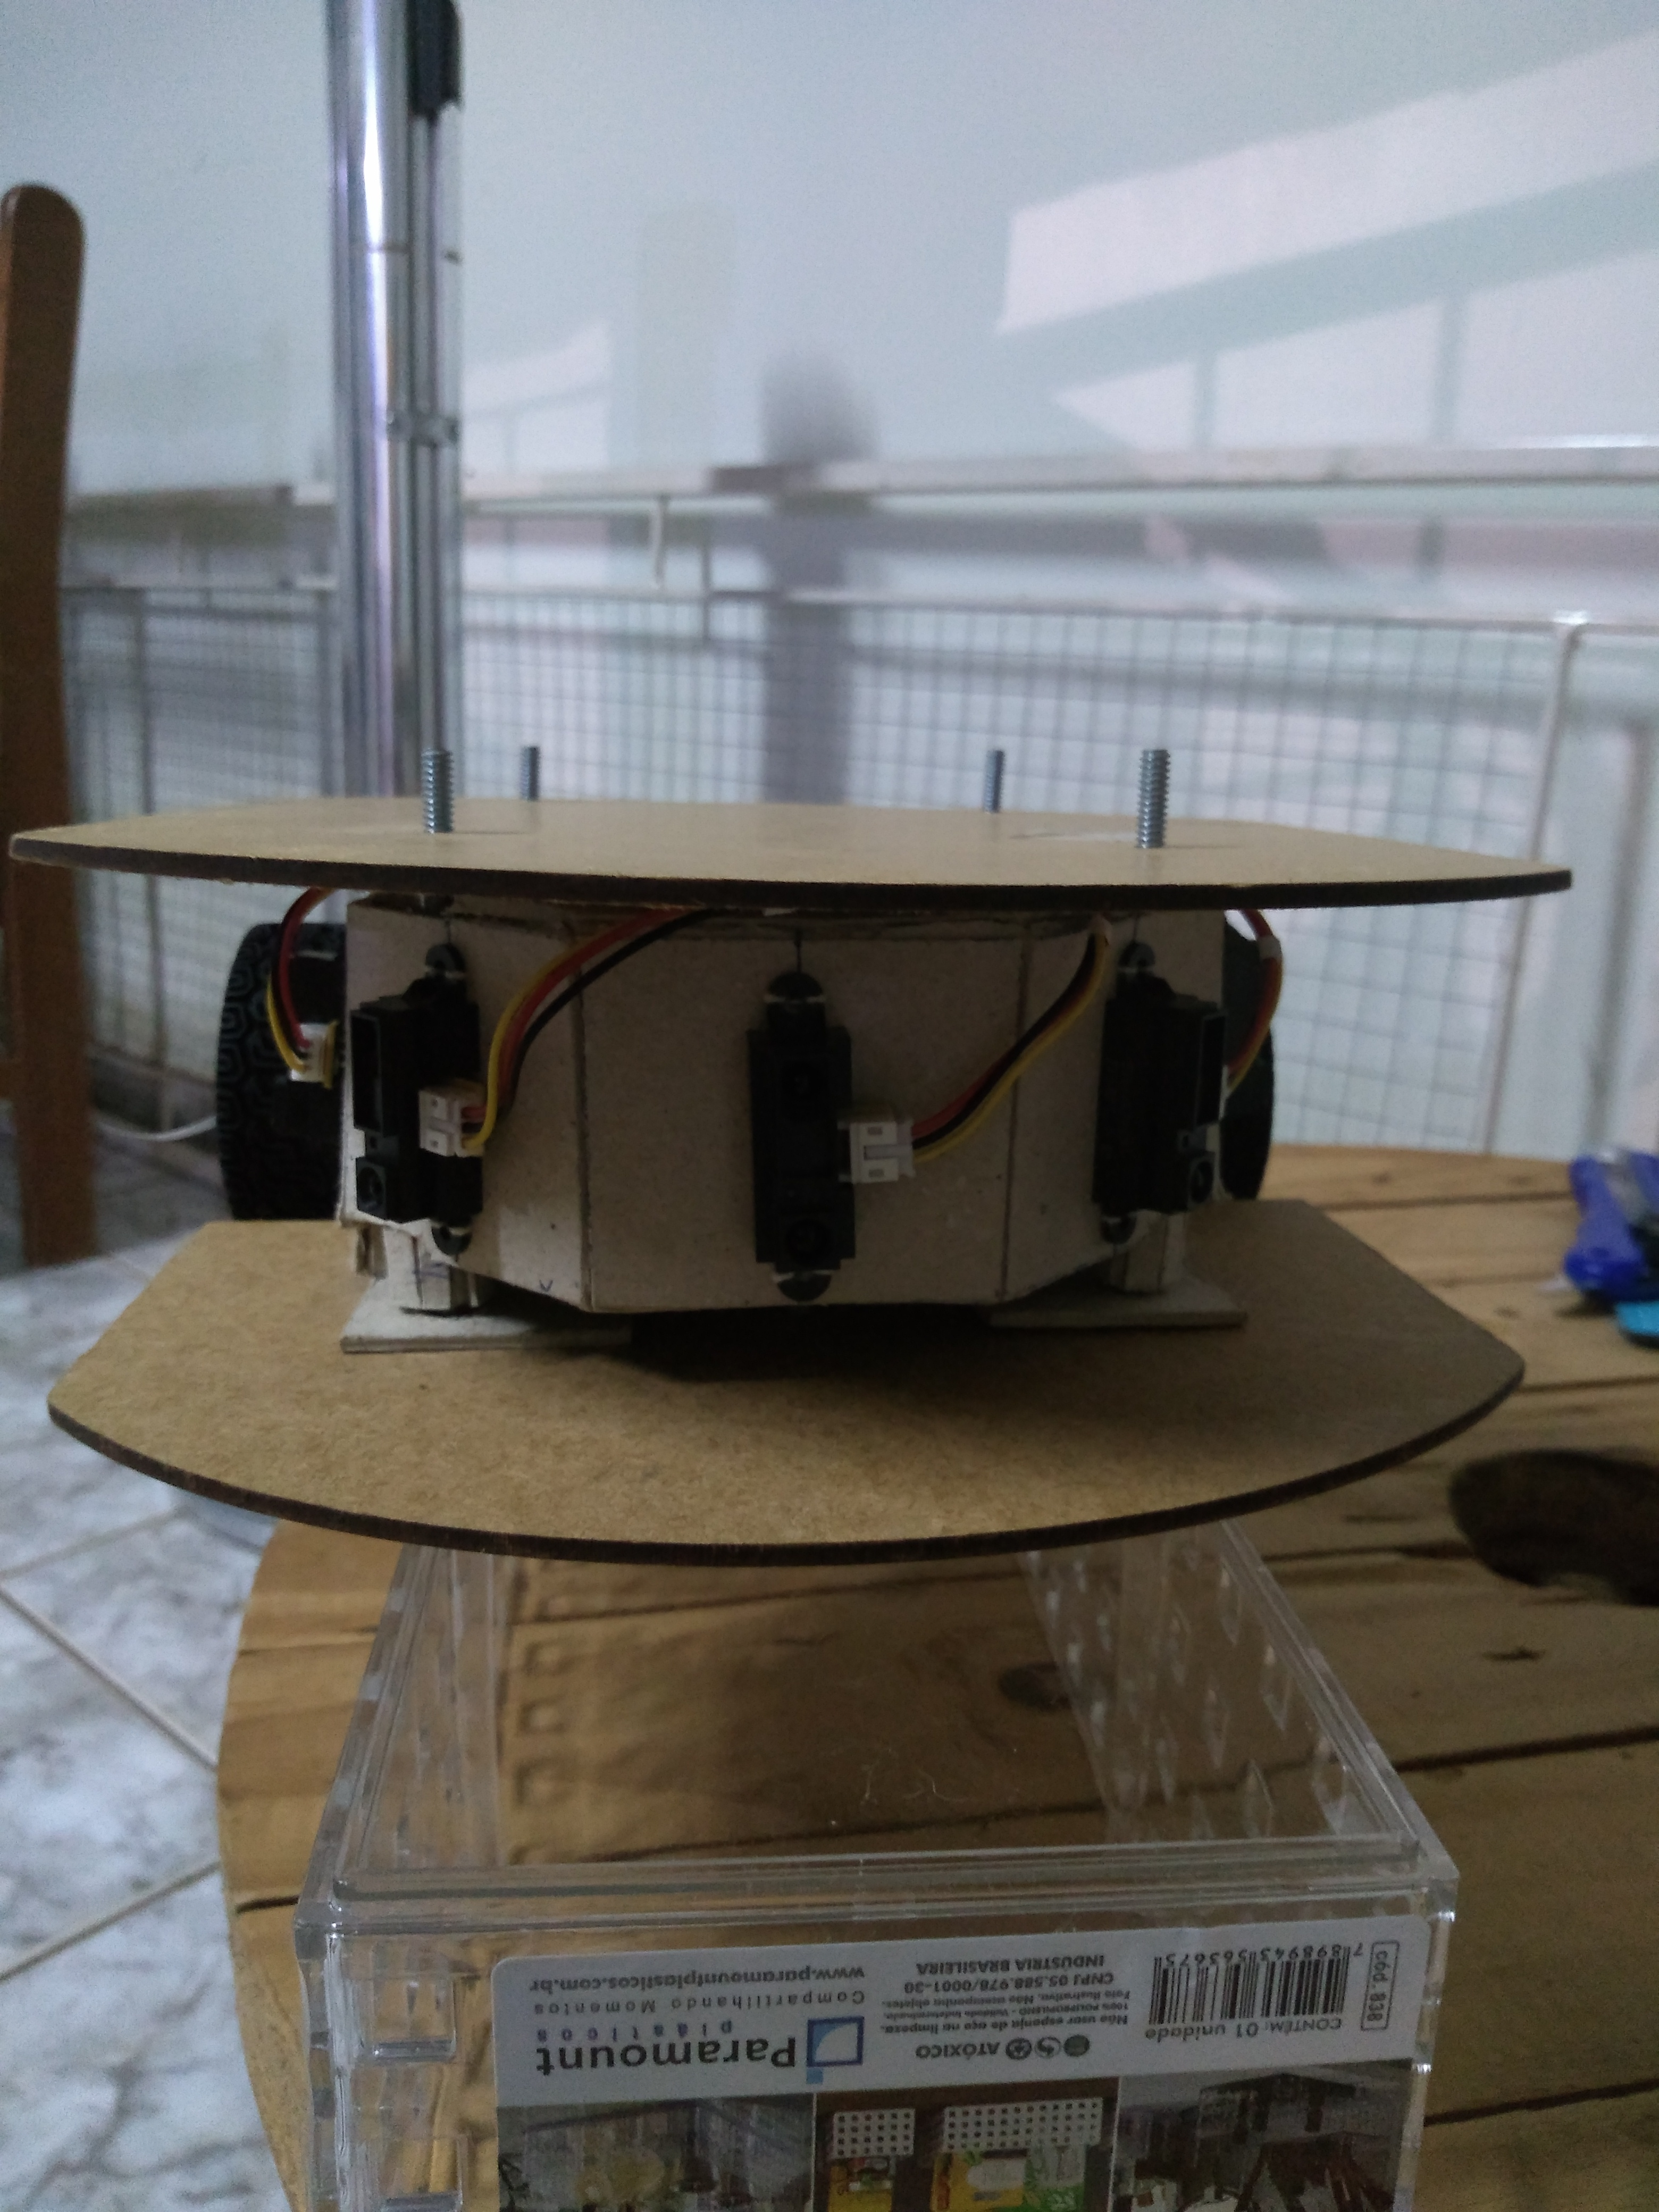
\includegraphics[trim={0cm 12.5cm 0cm 22.5cm}, clip, 
		scale=0.055]{Figuras/RoboMontagem6}%
		\subcaption{Robô montado}%
	\end{subfigure}%
\end{figure}
\end{frame}

\begin{frame}
	\frametitle{Curva para motores}
	\begin{figure}[!ht]
\centering
\caption{Curva do motor sem carga}
		\centering
		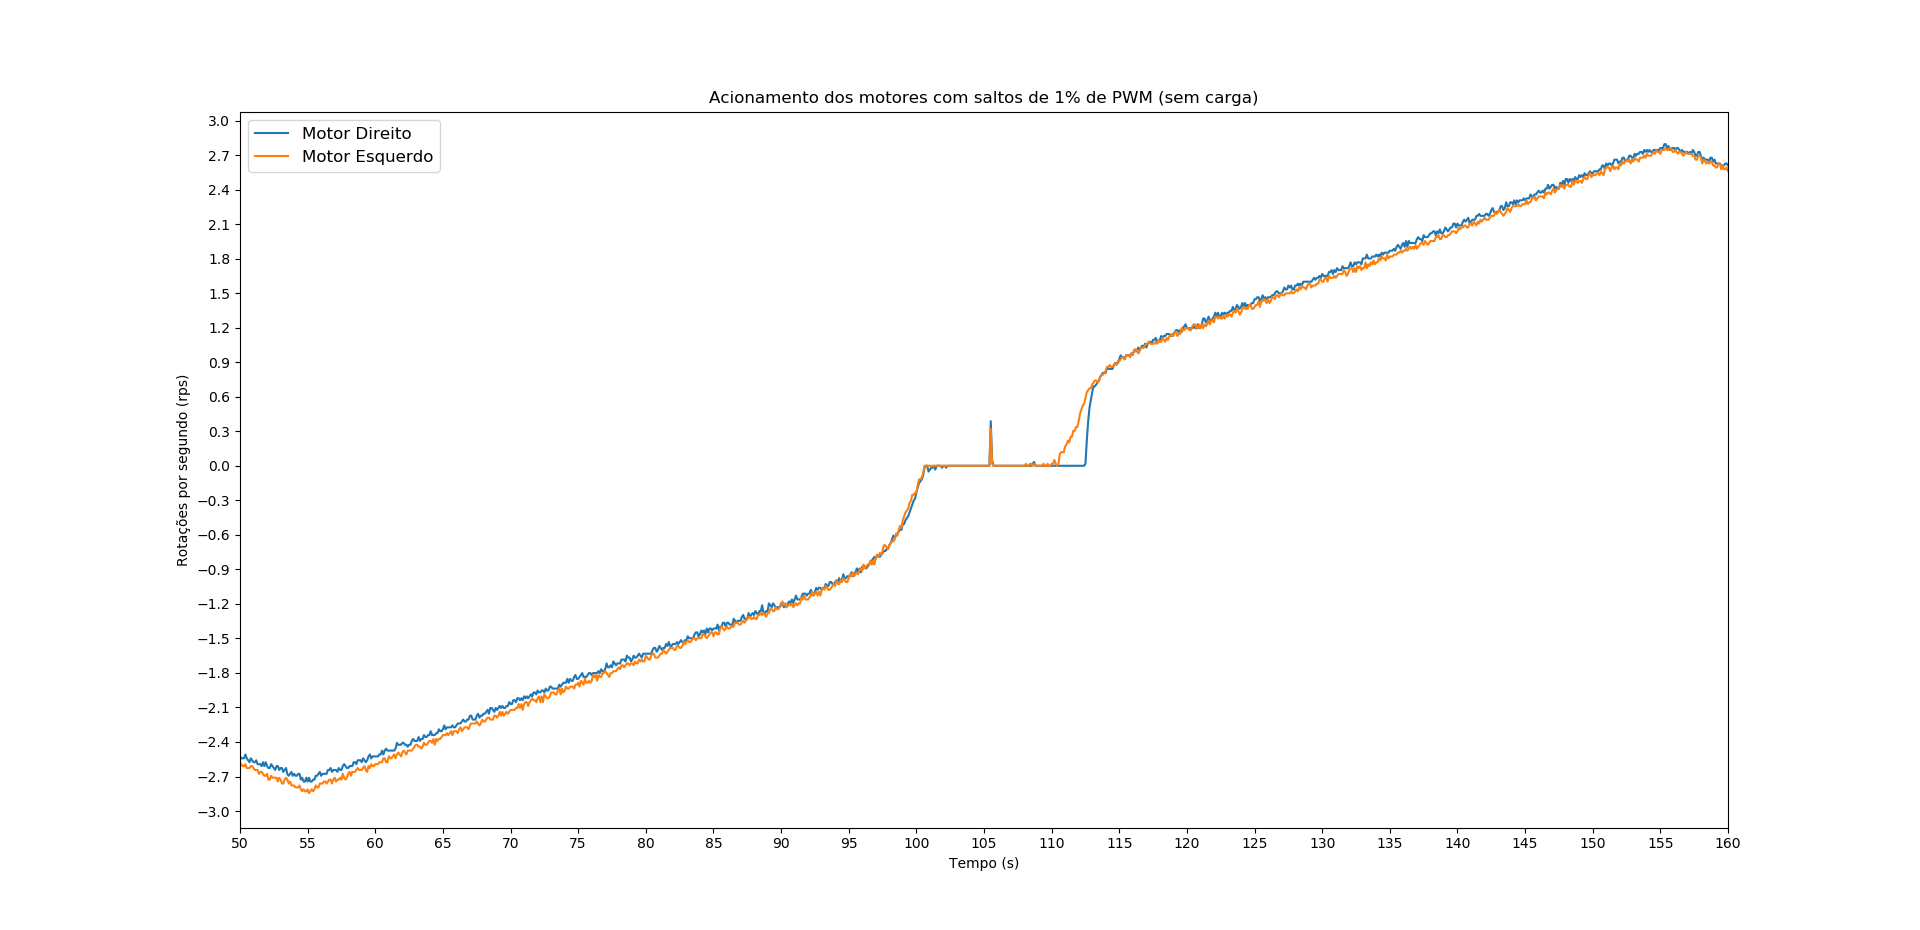
\includegraphics[trim={5cm 1cm 5cm 2cm},clip,
scale=0.25]{Figuras/Acionamento_Sem_Carga_rps}
\end{figure}
\end{frame}

\begin{frame}
	\begin{figure}[!ht]
\centering
\caption{Curva do motor com carga}
		\centering
		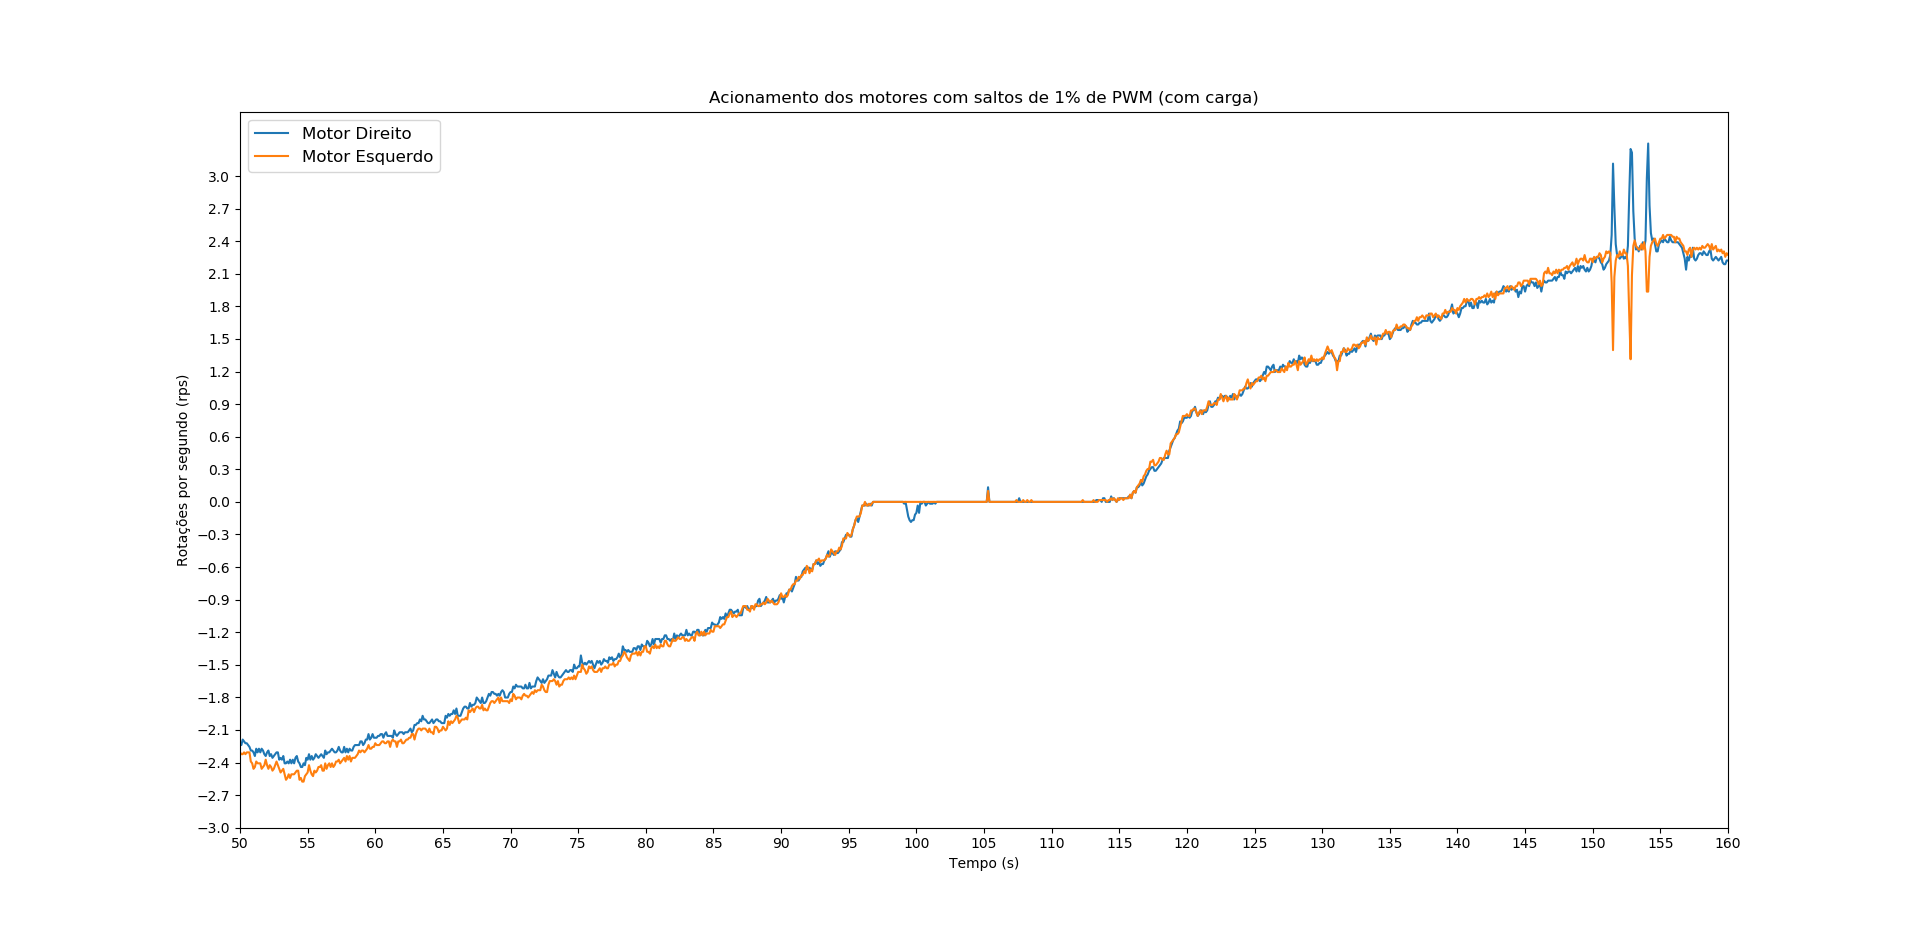
\includegraphics[trim={5cm 1cm 5cm 2cm},clip,
scale=0.25]{Figuras/Acionamento_Com_Carga_rps}
\end{figure}
\end{frame}

\begin{frame}
	\begin{figure}[!ht]
\centering
\caption{Regressão Linear para a curva do motor}
		\centering
		% fbox{}
		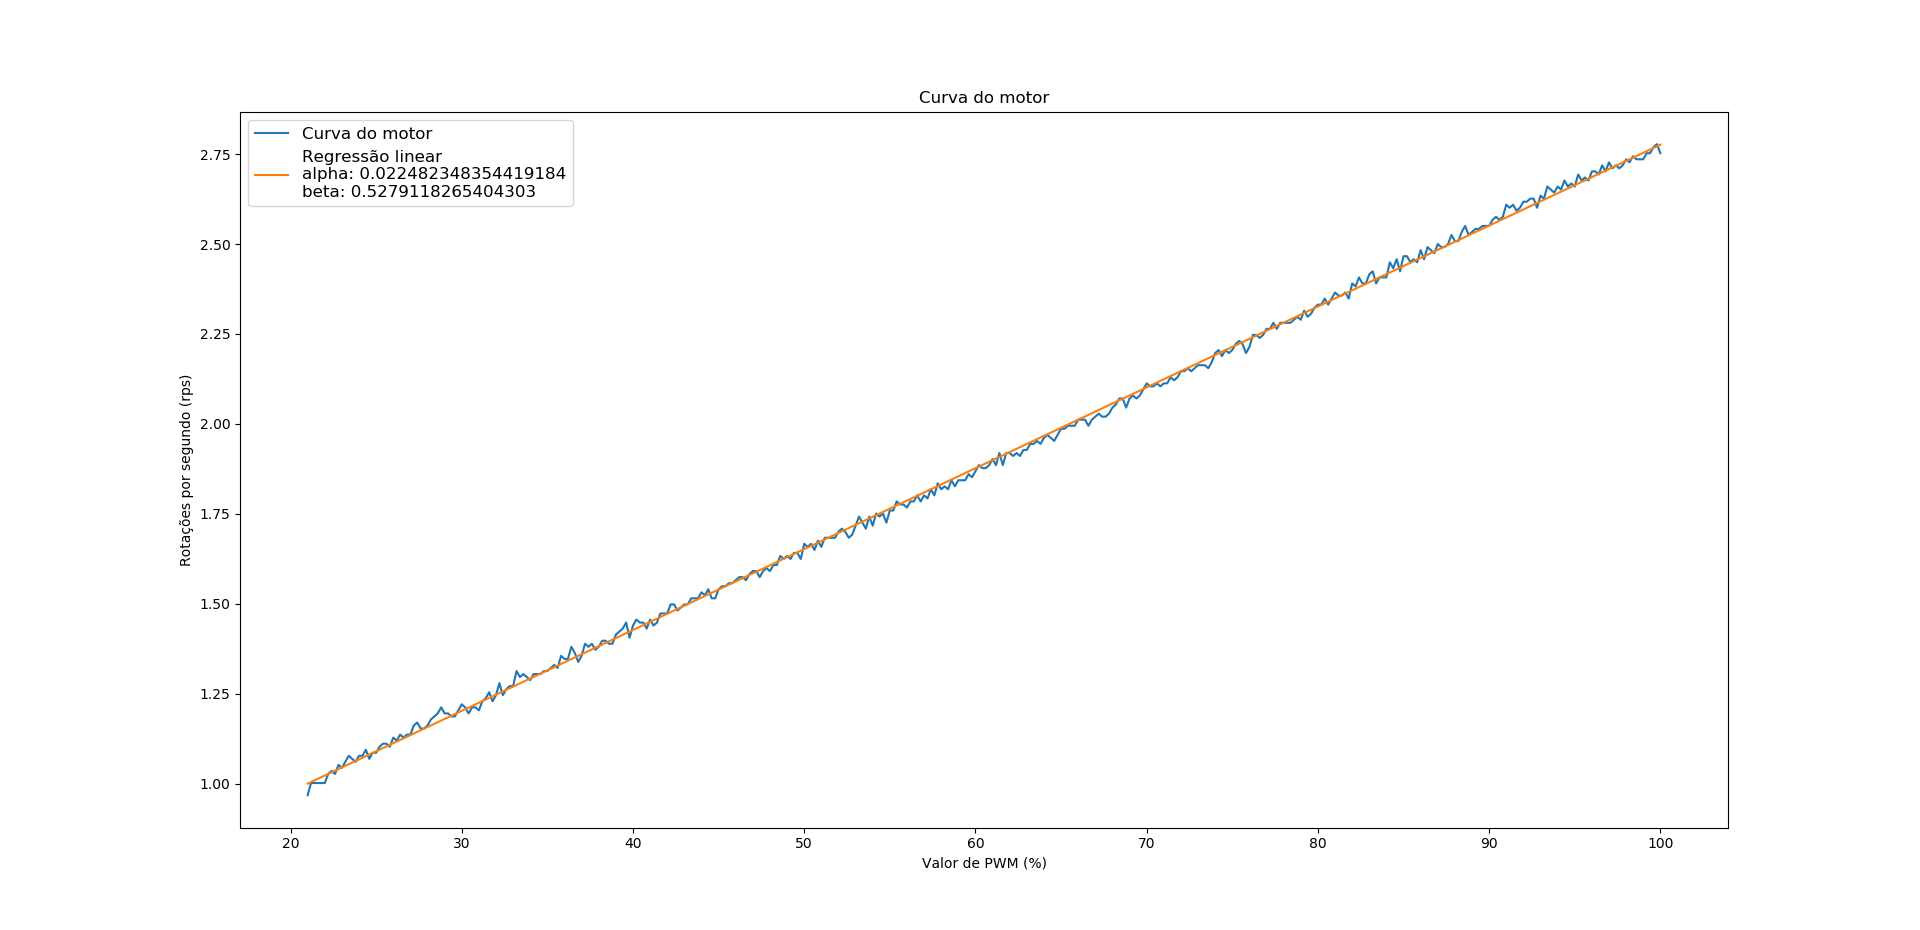
\includegraphics[trim={5cm 1cm 5cm 2cm},clip,
scale=0.25]{Figuras/Curva_Do_Motor_rps}
\end{figure}
\end{frame}
	
%%%%%%%%%%%%%%%%%%%%%%%%%%%%%
\begin{frame}
	\frametitle{Desenvolvimento}
	\begin{block}{Controlador Híbrido}
		Implementa arbitragem de comportamentos.
	\end{block}
	
	\begin{exampleblock}{Controlador Fuzzy}
		Implementa fusão de comportamentos.
	\end{exampleblock}
\end{frame}

\begin{frame}
	\frametitle{Controlador Híbrido}
	\begin{exampleblock}{Controlador PID}
		\begin{equation}
			\omega = K_p \epsilon(k) + K_i \sum_0^k \epsilon(k) T + k_d \frac{\epsilon(k) - \epsilon(k-1)}{T}
		\end{equation}
	\end{exampleblock}
	
	\onslide<2>
	\begin{block}{Considerações}
		\begin{itemize}
		  \item Velocidade angular tem prioridade sobre velocidade linear.
		  \item É necessário sacrificar velocidade linear em caso de saturação.
		\end{itemize}
	\end{block}
\end{frame}
	
\begin{frame}
	\begin{block}{Algoritmo para conversão de modelos}
	\vspace{-0.45cm}
	\begin{algorithm}[H]
		\algsetup{linenosize=\tiny}
		\scriptsize
		\caption{Uniciclo para Acionamento Diferencial priorizando $\omega$}
		\begin{algorithmic}[1]
			\onslide<1>
			\REQUIRE $v, \omega$
			\ENSURE $\omega_l, \omega_r$
			
			\IF{$v > 0$}
				\STATE $vlim \leftarrow max(min(abs(v), R \cdot VEL\_MAX), R \cdot VEL\_MIN)$
				\STATE $wlim \leftarrow max(min(abs(\omega), (R/L) \cdot (VEL\_MAX - VEL\_MIN)), 0)$
				
				\STATE $w_{l,lim}, w_{r,lim} \leftarrow uniToDiff(vlim, wlim)$
				
				\STATE $ velocidadeMaior \leftarrow max(w_{l,lim}, w_{r,lim})$
				\STATE $ velocidadeMenor \leftarrow min(w_{l,lim}, w_{r,lim})$
			
				\IF{$velocidadeMaior > VEL\_MAX$}
					\STATE $w_{l,lim} \leftarrow w_{l,lim} - (velocidadeMaior - VEL\_MAX)$
					\STATE $w_{r,lim} \leftarrow w_{r,lim} - (velocidadeMaior - VEL\_MAX)$
				\ELSIF{$velocidadeMenor < VEL\_MIN$}
					\STATE $w_{l,lim} \leftarrow w_{l,lim} + (VEL\_MIN - velocidadeMenor)$
					\STATE $w_{r,lim} \leftarrow w_{r,lim} + (VEL\_MIN - velocidadeMenor)$
				\ENDIF
				
				\IF{$v \geq 0$}
					\STATE $vlim \leftarrow 1$
				\ELSE
					\STATE $vlim \leftarrow -1$
				\ENDIF
				
				\onslide<2>
				\vspace{-6.5cm}
				\IF{$\omega \geq 0$}
					\STATE $wlim \leftarrow 1$
				\ELSE
					\STATE $wlim \leftarrow -1$
				\ENDIF
					
				\STATE $v,\omega \leftarrow diffToUni(w_{l,lim},w_{r,lim})$
				\STATE $v \leftarrow v \cdot vlim$
				\STATE $\omega \leftarrow \omega \cdot wlim$
			\ELSE
				\IF{$abs(\omega) > (R/L) \cdot 2 \cdot VEL\_MIN$}
					\IF{$\omega \geq 0$}
						\STATE $\omega \leftarrow max(min(abs(\omega),(R/L) \cdot 2 \cdot VEL\_MAX),(R/L) \cdot 2 \cdot VEL\_MIN)$ 
					\ELSE
						\STATE $\omega \leftarrow -max(min(abs(\omega),(R/L) \cdot 2 \cdot VEL\_MAX),(R/L) \cdot 2 \cdot VEL\_MIN)$
					\ENDIF
				\ELSE
					\STATE $\omega \leftarrow 0$
				\ENDIF
			\ENDIF
				
			\STATE $\omega_l, \omega_r \leftarrow uniToDiff(v,\omega)$
		\end{algorithmic}
	\end{algorithm}
	\end{block}
\end{frame}

\begin{frame}
	\frametitle{Comportamento Ir Para Objetivo (IPO)}
	\newcommand{\meuRoboLindaoCompIPO}{
	\begin{tikzpicture}[scale = 1.5]%
		\coordsystwo{I}
		\begin{scope}[shift={(3, 0.9)}]
			\draw[->] (0.3,0) arc (0:30:0.3);
			\draw[-] (0,0) -- (0.4,0);
			\node at (0.5,0.1) {$\phi$};
			
			% Pr 
			\begin{scope}[scale = 0.5]
				\node[color = gray] at (0.1,-0.35) {$P_r$};
			\end{scope}
			\begin{scope}[rotate=30,scale=0.5]
				\begin{scope}[scale=0.9]
					\coordsystwo{R}
				\end{scope}
				\begin{scope}[shift={(0.25,0)},rotate = -90]
					\RoboDiffClean
				\end{scope}
			\end{scope}	
		\end{scope}
		
		% Coord objetivo
		\begin{scope}[shift={(4, 3)}]
			\filldraw (0,0) circle (1pt);
			% Po
			\begin{scope}[scale = 0.5]
				\node[color = gray] at (0.2,-0.45) {$P_o$};
			\end{scope}
		\end{scope}
		
		% retas
		\node[inner sep = 3pt] (P1) at (4,3) {};
		\node[inner sep = 3pt] (P2) at (3,0.9) {};
		
		\draw[->] (0,0) -- (P1);
		\draw[->] (0,0) -- (P2);
		\draw[->] (P2) -- (P1);
		
		% angulo do objetivo
		\draw[->] (0.6,0) arc (0:37:0.6);
		\draw[-] (0,0) -- (0.4,0);
		\node at (0.8,0.4) {$\theta$};
	\end{tikzpicture}%
}%

\begin{figure}[ht]
	\centering%
	\caption{Comportamento Ir para Objetivo}%
	\meuRoboLindaoCompIPO
\end{figure}
\end{frame}

\begin{frame}
	\begin{exampleblock}{Equações para Comportamento IPO}
		\begin{equation}
			\mathbf{u_{ipo}} = P_o - P_r
		\end{equation}
		
		\pause
		\begin{equation}
			e_\theta = atan2(u_{ipo,y}, u_{ipo,x}) - \phi
		\end{equation}
		
		\pause
		\begin{itemize}
		  \item $K_p = 4$
		  \pause
		  \item $K_i = 0,01$
		  \pause
		  \item $K_d = 0,01$
		\end{itemize}
	\end{exampleblock}
\end{frame}

\begin{frame}
	\frametitle{Comportamento Evitar Obstáculo (EO)}
	\newcommand{\meuRoboLindaoCompEO}{

	\begin{scope}[shift={(0,0.3)}]
		% Pr 
		\begin{scope}[shift={(0,-0.3)}, scale = 0.5]
			\node[color = gray] at (0.1,-0.35) {$P_r$};
		\end{scope}
		\begin{scope}[rotate=90,scale=0.5]
			\filldraw (0,0) circle (0.5pt);
			\begin{scope}[shift={(0.25,0)},rotate = -90]
				\RoboDiffClean
			\end{scope}
		\end{scope}
	\end{scope}
		
	% Obstáculo
	\begin{scope}[shift={(2,0)}]
		\obstaculo{3}
	\end{scope}
}%

\newcommand{\obstaculo}[1]{
	\node[inner sep = 0pt] (P1) at (0,0) {};
	\node[inner sep = 0pt] (P2) at (0.5,0) {};
	\node[inner sep = 0pt] (P3) at (0.5,#1) {};
	\node[inner sep = 0pt] (P4) at (0,#1) {};
	\draw (P1) -- (P2);
	\draw (P2) -- (P3);
	\draw (P3) -- (P4);
	\draw (P4) -- (P1);
}

\newcommand{\sensorVisaoTriangular}[1]{
	\draw (0,0) -- (-0.1,#1);
	\draw (0,0) -- (0.1,#1);
	\draw (-0.1,#1) -- (0.1,#1);
}

\newcommand{\sensorVisaoVetor}[1]{
	\draw[->] (0,0) -- (0,#1);
}

\newcommand{\desenharSensoresTriangulo}{
	\node[color = gray] at (-2.58,0.6) {$d_1$};
	\node[color = gray] at (-1.82,2.41) {$d_2$};
	\node[color = gray] at (0,3.07) {$d_3$};
	\node[color = gray] at (1.82,2.41) {$d_4$};
	\node[color = gray] at (2.24,0.6) {$d_5$};
	
	\begin{scope}[shift={(0.38,0.6)},rotate=-90]
		\sensorVisaoTriangular{2-0.38}
	\end{scope}
	\begin{scope}[shift={(-0.38,0.6)},rotate=90]
		\sensorVisaoTriangular{2}
	\end{scope}
	\begin{scope}[shift={(0.28,0.77)},rotate=-45]
		\sensorVisaoTriangular{2}
	\end{scope}
	\begin{scope}[shift={(-0.28,0.77)},rotate=45]
		\sensorVisaoTriangular{2}
	\end{scope}	
	\begin{scope}[shift={(0,0.87)},rotate=0]
		\sensorVisaoTriangular{2}
	\end{scope}
}

\newcommand{\desenharSensoresVetores}{
	\node[color = gray] at (-2.58,0.6) {$v_1$};
	\node[color = gray] at (-1.82,2.41) {$v_2$};
	\node[color = gray] at (0,3.07) {$v_3$};
	\node[color = gray] at (1.82,2.41) {$v_4$};
	\node[color = gray] at (2.24,0.6) {$v_5$};
	
	\begin{scope}[shift={(0.38,0.6)},rotate=-90]
		\sensorVisaoVetor{2-0.38}
	\end{scope}
	\begin{scope}[shift={(-0.38,0.6)},rotate=90]
		\sensorVisaoVetor{2}
	\end{scope}
	\begin{scope}[shift={(0.28,0.77)},rotate=-45]
		\sensorVisaoVetor{2}
	\end{scope}
	\begin{scope}[shift={(-0.28,0.77)},rotate=45]
		\sensorVisaoVetor{2}
	\end{scope}	
	\begin{scope}[shift={(0,0.87)},rotate=0]
		\sensorVisaoVetor{2}
	\end{scope}
}


\begin{figure}[ht]
	\centering%
	\begin{subfigure}[t]{0.5\textwidth}%
		\centering%
			
		\begin{tikzpicture}[scale = 1.1]%
			\meuRoboLindaoCompEO
			\desenharSensoresTriangulo
		\end{tikzpicture}%
		
		\caption{Sensores infravermelho}%
	\end{subfigure}%
	~
	\begin{subfigure}[t]{0.5\textwidth}%
		\centering%
		
		\begin{tikzpicture}[scale = 1.1]%
			\meuRoboLindaoCompEO
			\desenharSensoresVetores
		\end{tikzpicture}%
			
		\caption{Vetores utilizados}%
	\end{subfigure}%
\end{figure}
\end{frame}

\begin{frame}
	\begin{block}{Conversão de sistemas de coordenadas}
		\begin{equation}
			\mleft[ 
			\begin{array}{c c}
				x \\ y
			\end{array}
			\mright]_i^R = \mleft[
			\begin{matrix}
		  		\cos{\theta_i} & -\sin{\theta_i} \\
		  		\sin{\theta_i} & \cos{\theta_i} \\
			\end{matrix}
			\mright] \mleft[ 
			\begin{array}{c c}
				d_i \\ 0
			\end{array}
			\mright] + \mleft[ 
			\begin{array}{c c}
				o_x \\ o_y
			\end{array}
			\mright]_i^R
		\end{equation}
	\end{block}
	
	\pause
	\begin{exampleblock}{Combinação Linear}
		\begin{equation}
			\mathbf{u_{eo2}} = k_1 \mathbf{v_1} + k_2 \mathbf{v_2} + k_3 \mathbf{v_3} + 
			k_4 \mathbf{v_4} + k_5 \mathbf{v_5}
		\end{equation}
	\end{exampleblock}
	
	\pause
	\begin{block}{Equilíbrio}
		\begin{equation}
			\mathbf{u_{eo1}} = k_1 \mathbf{v_1} + k_2 \mathbf{v_2} + k_3 \mathbf{v_3} + 
			k_4 \mathbf{v_4} + k_5 \mathbf{v_5} + \mathbf{v_{eq}}
		\end{equation}
	\end{block}
\end{frame}

\begin{frame}
	\begin{block}{Parâmetros}
		\begin{itemize}
		  \item Constantes $k_i$:
			  \subitem{$k_1 = 0,7$}
			  \subitem{$k_2 = 2$}
			  \subitem{$k_3 = 1,2$}
			  \subitem{$k_4 = 2$} 
			  \subitem{$k_5 = 0,7$}
		  \pause
		  \item $\mathbf{v_{eq}} = [-240 \ 0]^T$
		  \pause
		  \item $D_{insegura} = 25$
		\end{itemize}
	\end{block}
\end{frame}

\begin{frame}
	\begin{exampleblock}{Comportamento EO completo}
		\begin{equation}
			\mathbf{u_{eo}} = 
			\begin{cases}
				\mathbf{u_{eo1}} & \text{para} \ | \mathbf{v_3} | \geq D_{insegura} \\
				
				\mleft[
				\begin{matrix}
		  			\cos{(90)} & -\sin{(90)} \\
		  			\sin{(90)} & \cos{(90)} \\
				\end{matrix}
				\mright] \mathbf{u_{eo2}} & 				
				\begin{matrix*}[l]
		  			\text{para} \ | \mathbf{v_3} | < D_{insegura} \ \land \\
		  			k_1 \ (|\mathbf{v_5}| - |\mathbf{v_1}|) + k_2 \ (|\mathbf{v_4}| - |\mathbf{v_2}|)
					> 0 \\
				\end{matrix*} \\
				
				\mleft[
				\begin{matrix}
		  			\cos{(-90)} & -\sin{(-90)} \\
		  			\sin{(-90)} & \cos{(-90)} \\
				\end{matrix}
				\mright] \mathbf{u_{eo2}} & 
				\begin{matrix*}[l]
		  			\text{para} \ | \mathbf{v_3} | < D_{insegura} \ \land \\
		  			k_1 \ (|\mathbf{v_5}| - |\mathbf{v_1}|) + k_2 \ (|\mathbf{v_4}| - |\mathbf{v_2}|)
					\leq 0 \\
				\end{matrix*} \\
			\end{cases}
		\end{equation}
	\end{exampleblock}
\end{frame}

\begin{frame}
	\frametitle{Comportamento Mesclado IPO + EO}
	\begin{block}{Cálculo da recomendação}
		\begin{equation}
			\mathbf{u_{eo\_e\_ipo}} = k \ \hat{\mathbf{u}}_{ipo} + (1-k) \ \hat{\mathbf{u}}_{eo}
		\end{equation}
		
		\pause
		\begin{itemize}
		  \item $k = 0,3$
		\end{itemize}
	\end{block}
	
	\pause
	\begin{exampleblock}{IPO}
		\begin{equation}
			\mathbf{u_{ipo}} = P_o - P_r
		\end{equation}
	\end{exampleblock}
	
	\pause
	\begin{block}{EO}
		\begin{equation}
			\mathbf{u_{eo1}} = k_1 \mathbf{v_1} + k_2 \mathbf{v_2} + k_3 \mathbf{v_3} + 
			k_4 \mathbf{v_4} + k_5 \mathbf{v_5} + \mathbf{v_{eq}}
		\end{equation}
	\end{block}
\end{frame}

\begin{frame}
	\frametitle{O problema dos Mínimos Locais}
	\newcommand{\meuRoboLindaoCompMinimos}{
	\begin{scope}[shift={(0,0.3)}]
		% Pr 
		\begin{scope}[shift={(0,-0.3)}, scale = 0.5]
			\node[color = gray] at (0.1,-0.35) {$P_r$};
		\end{scope}
		\begin{scope}[rotate=90,scale=0.5]
			\filldraw (0,0) circle (0.5pt);
			\begin{scope}[shift={(0.25,0)},rotate = -90]
				\RoboDiffClean
			\end{scope}
		\end{scope}
	\end{scope}
}%

\newcommand{\obstaculoA}[2]{
	\node[inner sep = 0pt] (P1) at (#1,0) {};
	\node[inner sep = 0pt] (P2) at (\fpeval{#1+(#2/2)},\fpeval{#2*sqrt{2}/2}) {};
	\node[inner sep = 0pt] (P3) at (\fpeval{#1+((3*#2)/2)},\fpeval{#2*sqrt{2}/2}) {};
	\node[inner sep = 0pt] (P4) at (\fpeval{#1+2*#2},0) {};
	\node[inner sep = 0pt] (P5) at (\fpeval{#1+((3*#2)/2)},\fpeval{-(#2*sqrt{2}/2)}) {};
	\node[inner sep = 0pt] (P6) at (\fpeval{#1+(#2/2)},\fpeval{-(#2*sqrt{2}/2)}) {};
	
	\draw[color = darkgray] (P1) -- (P2);
	\draw[color = darkgray] (P2) -- (P3);
	\draw[color = darkgray] (P3) -- (P4);
	\draw[color = darkgray] (P4) -- (P5);
	\draw[color = darkgray] (P5) -- (P6);
	\draw[color = darkgray] (P6) -- (P1);
	
	\node[color = gray] at (#1+#2,-1.3) {Obstáculo 1};
}

\newcommand{\obstaculoB}[3]{
	\node[inner sep = 0pt] (P1) at (#1,#2) {};
	\node[inner sep = 0pt] (P2) at (#1,#2+0.5) {};
	\node[inner sep = 0pt] (P3) at (#1+#3+0.5,#2+0.5) {};
	\node[inner sep = 0pt] (P4) at (#1+#3+0.5,-#2-0.5) {};
	
	\node[inner sep = 0pt] (P5) at (#1,-#2-0.5) {};
	\node[inner sep = 0pt] (P6) at (#1,-#2) {};
	\node[inner sep = 0pt] (P7) at (#1+#3,-#2) {};
	\node[inner sep = 0pt] (P8) at (#1+#3,#2) {};
	
	\draw[color = darkgray] (P1) -- (P2);
	\draw[color = darkgray] (P2) -- (P3);
	\draw[color = darkgray] (P3) -- (P4);
	\draw[color = darkgray] (P4) -- (P5);
	\draw[color = darkgray] (P5) -- (P6);
	\draw[color = darkgray] (P6) -- (P7);
	\draw[color = darkgray] (P7) -- (P8);
	\draw[color = darkgray] (P8) -- (P1);
	
	\node[color = gray] at (#1+0.25+#3/2,-2.8) {Obstáculo 2};
}

\newcommand{\obstaculoC}[2]{
	\node[inner sep = 0pt] (P1) at (#1,#2+0.5) {};
	\node[inner sep = 0pt] (P2) at (#1+0.5,#2+0.5) {};
	\node[inner sep = 0pt] (P3) at (#1+0.5,-#2-0.5) {};
	\node[inner sep = 0pt] (P4) at (#1,-#2-0.5) {};
	
	\draw[color = darkgray] (P1) -- (P2);
	\draw[color = darkgray] (P2) -- (P3);
	\draw[color = darkgray] (P3) -- (P4);
	\draw[color = darkgray] (P4) -- (P1);
	
	\node[color = gray] at (#1+0.25,-2.8) {Obstáculo 3};
}

\begin{figure}[ht]
	\centering%
	
	\begin{tikzpicture}[scale = 1.1]%
		% Robô
		\begin{scope}[rotate=-90]
			\meuRoboLindaoCompMinimos
		\end{scope}
		\obstaculoA{2}{1.5}
		\obstaculoB{4}{2}{2}
		\obstaculoC{8}{2}
		
		\begin{scope}[shift={(10,0)}]
			\filldraw (0,0) circle (1.5pt);
			\node[color = gray] at (0,-0.35) {Objetivo};
		\end{scope}
	\end{tikzpicture}%
\end{figure}
\end{frame}

\begin{frame}
	\frametitle{Comportamento Seguir Parede}
	\newcommand{\parede}[2]{
	\node[inner sep = 0pt] (P1) at (0,0) {};
	\node[inner sep = 0pt] (P2) at (#2,0) {};
	\node[inner sep = 0pt] (P3) at (#2,0.5) {};
	\node[inner sep = 0pt] (P4) at (0.5,0.5) {};
	\node[inner sep = 0pt] (P5) at (0.5,#1) {};
	\node[inner sep = 0pt] (P6) at (0,#1) {};
	\draw[color = darkgray] (P1) -- (P2);
	\draw[color = darkgray] (P2) -- (P3);
	\draw[color = darkgray] (P3) -- (P4);
	\draw[color = darkgray] (P4) -- (P5);
	\draw[color = darkgray] (P5) -- (P6);
	\draw[color = darkgray] (P6) -- (P1);
}

\newcommand{\sensorVisaoVetorSp}[1]{
	\draw[->] (0,0) -- (0,#1);
}

\newcommand{\desenharSensoresTrianguloSPb}{
	\begin{scope}[shift={(0.38,0.6)},rotate=-90]
		\sensorVisaoTriangularSp{2-0.9}
	\end{scope}
	\begin{scope}[shift={(-0.38,0.6)},rotate=90]
		\sensorVisaoTriangularSp{2}
	\end{scope}
	\begin{scope}[shift={(0.28,0.77)},rotate=-45]
		\sensorVisaoTriangularSp{2-0.5}
	\end{scope}
	\begin{scope}[shift={(-0.28,0.77)},rotate=45]
		\sensorVisaoTriangularSp{2}
	\end{scope}	
	\begin{scope}[shift={(0,0.87)},rotate=0]
		\sensorVisaoTriangularSp{2-1}
	\end{scope}
}

\newcommand{\desenharLinhasParedeA}{
	\begin{scope}[shift={(-0.38,0.6)},rotate=90]
		\begin{scope}[shift={(0,2-1.3)}]
			\node[inner sep = 0pt] (P1) at (0,0) {};
		\end{scope}
	\end{scope}
	\begin{scope}[shift={(-0.28,0.77)},rotate=45]
		\begin{scope}[shift={(0,2)}]
			\node[inner sep = 0pt] (P2) at (0,0) {};
		\end{scope}
	\end{scope}
	
	\draw (P1) -- (P2);
}

\newcommand{\desenharLinhasParedeB}{
	\begin{scope}[shift={(0.38,0.6)},rotate=-90]
		\begin{scope}[shift={(0,2-0.9)}]
			\node[inner sep = 0pt] (P1) at (0,0) {};
		\end{scope}
	\end{scope}
	\begin{scope}[shift={(0,0.87)},rotate=0]
		\begin{scope}[shift={(0,2-1)}]
			\node[inner sep = 0pt] (P2) at (0,0) {};
		\end{scope}
	\end{scope}
	
	\draw (P1) -- (P2);
}

\begin{figure}[ht]
	\centering%
	\begin{subfigure}[t]{0.5\textwidth}%
		\centering%
		\begin{tikzpicture}[scale = 1.1]%
			% Obstáculo
			\parede{3}{2}
			% Robô
			\begin{scope}[shift={(-1.1,1.4)},rotate=180]
				\meuRoboLindaoCompSP
				\desenharSensoresTrianguloSPa
				\desenharLinhasParedeA
			\end{scope}
		\end{tikzpicture}%
		
		\caption{Parede subestimada}%
	\end{subfigure}%
	~
	\begin{subfigure}[t]{0.5\textwidth}%
		\centering%
		\begin{tikzpicture}[scale = 1.1]%
			% Obstáculo
			\begin{scope}[shift={(0,0)},xscale=-1,yscale=1]
				\parede{3}{4}
			\end{scope}
			% Robô
			\begin{scope}[shift={(-2.4,2)},rotate=-90]
				\meuRoboLindaoCompSP
				\desenharSensoresTrianguloSPb
				\desenharLinhasParedeB
			\end{scope}
		\end{tikzpicture}%
			
		\caption{Parede superestimada}%
	\end{subfigure}%
\end{figure}
\end{frame}

\begin{frame}
	\newcommand{\desenharLinhasParedeC}[2]{
	\begin{scope}[shift={(-0.38,0.6)},rotate=90]
		\begin{scope}[shift={(0,2-1.3)}]
			\node[inner sep = 0pt] (P1) at (0,0) {};
		\end{scope}
	\end{scope}
	\begin{scope}[shift={(-0.28,0.77)},rotate=45]
		\begin{scope}[shift={(0,2)}]
			\node[inner sep = 0pt] (P2) at (0,0) {};
		\end{scope}
	\end{scope}
	
	\draw (P1) -- (P2);
	
	% linhas continuacao:
	\def\UserVetAX{-1.08}
	\def\UserVetAY{0.6}
	
	\def\UserVetXNum{\fpeval{-0.28-sqrt(2)+1.08}}
	\def\UserVetYNum{\fpeval{0.77+sqrt(2)-0.6}}
	\def\UserVetMod{\fpeval{sqrt(\UserVetXNum*\UserVetXNum + \UserVetYNum*\UserVetYNum)}}
	
	\def\UserVetX{\fpeval{\UserVetXNum/\UserVetMod}}
	\def\UserVetY{\fpeval{\UserVetYNum/\UserVetMod}}
	
	\def\UserLinhaTrasX{\fpeval{-1.08 -\UserVetX*#1}}
	\def\UserLinhaTrasY{\fpeval{0.6 -\UserVetY*#1}}
	\def\UserLinhaFrenteX{\fpeval{-0.28-sqrt(2) +\UserVetX*#2}}
	\def\UserLinhaFrenteY{\fpeval{0.77+sqrt(2) +\UserVetY*#2}}
			
	\draw [dashed] (P1) -- (\UserLinhaTrasX,\UserLinhaTrasY);
	\draw [dashed] (P2) -- (\UserLinhaFrenteX,\UserLinhaFrenteY);
	
	\def\distance{\fpeval{\UserVetX * \UserVetAX + \UserVetY * (\UserVetAY - 0.3)}}
	\begin{scope}[shift={(0,0.3)}]
		\def\UserVetPerpX{\fpeval{\UserVetAX-\distance*\UserVetX}}
		\def\UserVetPerpY{\fpeval{(\UserVetAY - 0.3)-\distance*\UserVetY}}
		\def\UserVetPerpNormX{\UserVetPerpX/(sqrt(\UserVetPerpX*\UserVetPerpX + \UserVetPerpY*\UserVetPerpY))}
		\def\UserVetPerpNormY{\UserVetPerpY/(sqrt(\UserVetPerpX*\UserVetPerpX + \UserVetPerpY*\UserVetPerpY))}
	
		\draw[-{Latex[length=2mm]}] (0,0) -- (P1) node [black,midway,yshift=-0.21cm,xshift=0.1cm] {$u_a$};
		\begin{scope}[shift={(P1)}]
			\draw[-{Latex[length=2mm]}] (0,0) -- (\UserVetX, \UserVetY) node [black,midway,xshift=-0.3cm,yshift=0.1cm] {$u_t$};
		\end{scope}
		\draw[-{Latex[length=2mm]}] (0,0) -- (\UserVetPerpX, \UserVetPerpY)
		node [black,midway,yshift=0.3cm,xshift=0.2] {$u_p$};

		\def\UserChavesX{\fpeval{\UserVetAX-\distance*\UserVetX}}
		\def\UserChavesY{\fpeval{(\UserVetAY - 0.3)-\distance*\UserVetY}}	
		\draw [decorate,decoration={brace,amplitude=10pt},xshift=-2pt,yshift=-2pt]
			(\UserChavesX, \UserChavesY) -- (\fpeval{-1.08},\fpeval{0.3}) 
			node [black,midway,xshift=0.6cm, yshift=0.1cm] {$d$};
			
		% angulo reto:
		\def\UserTamanhoQuad{0.15}
		\def\UserPontoEsqX{\fpeval{\UserVetPerpX - \UserTamanhoQuad*\UserVetPerpNormX}}
		\def\UserPontoEsqY{\fpeval{\UserVetPerpY - \UserTamanhoQuad*\UserVetPerpNormY}}
		\def\UserPontoDirX{\fpeval{\UserVetPerpX + \UserTamanhoQuad*\UserVetX}}
		\def\UserPontoDirY{\fpeval{\UserVetPerpY + \UserTamanhoQuad*\UserVetY}}
		\def\UserPontoBaixoX{\fpeval{\UserVetPerpX - \UserTamanhoQuad*\UserVetPerpNormX + \UserTamanhoQuad*\UserVetX}}
		\def\UserPontoBaixoY{\fpeval{\UserVetPerpY - \UserTamanhoQuad*\UserVetPerpNormY + \UserTamanhoQuad*\UserVetY}}
		
		\draw (\UserVetPerpX, \UserVetPerpY) -- (\UserPontoEsqX, \UserPontoEsqY);
		\draw (\UserVetPerpX, \UserVetPerpY) -- (\UserPontoDirX, \UserPontoDirY);
		\draw (\UserPontoEsqX, \UserPontoEsqY) -- (\UserPontoBaixoX, \UserPontoBaixoY);
		\draw (\UserPontoDirX, \UserPontoDirY) -- (\UserPontoBaixoX, \UserPontoBaixoY);
		
		\filldraw (\fpeval{\UserVetPerpX - \UserTamanhoQuad*\UserVetPerpNormX/2 + \UserTamanhoQuad*\UserVetX/2}, 
		\fpeval{\UserVetPerpY - \UserTamanhoQuad*\UserVetPerpNormY/2 + \UserTamanhoQuad*\UserVetY/2}) circle (0.5pt);
		
		% Ângulo vetor
		\begin{scope}[shift={(P1)}, rotate=180]
			\draw (0.3*\UserVetX,0.3*\UserVetY) arc (110:160:0.3);
			\node at (-0.35,0.25) {\footnotesize $\theta$};
		\end{scope}
	\end{scope}
}

\begin{figure}[ht]
	\centering%	
	\begin{tikzpicture}[scale = 1.1]%
		% Obstáculo
		%\parede{3}{2}
		% Robô
		\begin{scope}[shift={(-1.1,1.4)},rotate=180]
			\meuRoboLindaoCompSP
			\desenharSensoresTrianguloSPa
			\desenharLinhasParedeC{3}{2}
		\end{scope}
	\end{tikzpicture}%
\end{figure}
\end{frame}

\begin{frame}
	\begin{block}{Equação para Comportamento Seguir Parede}
		\begin{equation}
			\mathbf{u_p} = \mathbf{u_a} - d \cdot \mathbf{u_t}
		\end{equation}
		
		\pause
		\begin{equation}
			\mathbf{u_a} \cdot \mathbf{u_t} = \mid \mathbf{u_a} \mid \cdot \mid \mathbf{u_t} \mid \cos(\theta)
		\end{equation}
		\pause
		\begin{equation}
			\mathbf{u_a} \cdot \mathbf{u_t} = \mid \mathbf{u_a} \mid \cos(\theta) = d
		\end{equation}
		
		\pause
		\begin{equation}
			\mathbf{u_{fw}} = \mathbf{u_t} + \beta \cdot \left(\mathbf{u_p} - d_{fw} \cdot 
			\frac{\mathbf{u_p}}{\mid \mathbf{u_p} \mid}\right)
		\end{equation}
	\end{block}
\end{frame}

\begin{frame}
	\begin{exampleblock}{Parâmetros}
		\begin{itemize}
		  \item $\beta = 5,5$
		  \pause
		  \item $d_{fw} = 50 cm$
		  \pause
		  \item Constantes do Controlador PID:
		  	\subitem{$k_p = 2$}
		  	\subitem{$k_i = 0$}
		  	\subitem{$k_d = 0$}
		\end{itemize}
	\end{exampleblock}
\end{frame}

\begin{frame}
	\frametitle{Autômato para arbitragem}
	\begin{block}{Estados}
		\begin{table}[ht]
\centering
\vspace{0.2 cm}
\begin{tabular}{|c|l|l|}
\hline
\textbf{Índice} & \textbf{Comportamento} & \textbf{Descrição}                                         \\ \hline
0      & P             & Parar                                             \\ \hline
1      & IPO           & Ir para Objetivo                                  \\ \hline
2      & EO            & Evitar Obstáculos                                 \\ \hline
3      & IPO E EO    & Ir para Objetivo e Evitar Obstáculos \\ \hline
4      & SP AH         & Seguir Parede sentido Anti-horário				   \\ \hline
5      & SP H          & Seguir Parede sentido Horário                     \\ \hline
\end{tabular}
\end{table}
	\end{block}
\end{frame}

\begin{frame}
	\begin{exampleblock}{Eventos}
		\begin{table}[ht]
\centering
\vspace{0.2 cm}
\begin{tabular}{|c|l|}
\hline
\textbf{Legenda} & \textbf{Condições}                  \\ \hline
a       & No objetivo                           \\ \hline
b       & Fez progresso                         \\ \hline
c       & Tem Obstáculo                         \\ \hline
d       & Está inseguro                         \\ \hline
e       & Livre de obstáculo                    \\ \hline
f       & Contornando pela esquerda            \\ \hline
g       & Contornando pela direita              \\ \hline
\end{tabular}
\end{table}
	\end{exampleblock}
\end{frame}

\begin{frame}
	\begin{block}{Evento No Objetivo (a)}
		\begin{equation}
			\mid \mathbf{v_{\text{objetivo}}} - \mathbf{v_{\text{robô}}} \mid < D_{STOP}
		\end{equation}
	\end{block}
	\pause
	\begin{exampleblock}{Parâmetro}
		\begin{itemize}
		  \item $D_{STOP} = 15$
		\end{itemize}
	\end{exampleblock}
\end{frame}

\begin{frame}
	\begin{exampleblock}{Evento Fez progresso (b)}
		
		\begin{algorithm}[H]
		\algsetup{linenosize=\tiny}
		\scriptsize
		\caption{Verificação de progresso}
		\begin{algorithmic}[1]
	
		\REQUIRE $d_{prog}, \mathbf{v_{\text{objetivo}}}, \mathbf{v_{\text{robô}}}$
		\ENSURE $d_{prog}, retornoBooleano$
	
		\IF{$\mid \mathbf{v_{\text{objetivo}}} - \mathbf{v_{\text{robô}}} \mid < (d_{prog} - D_{PROG\_EPSILON})$}
			\STATE $d_{prog} \leftarrow min(\mid \mathbf{v_{\text{objetivo}}} - \mathbf{v_{\text{robô}}} \mid, d_{prog})$
			\STATE $retornoBooleano \leftarrow Verdadeiro$
		\ELSIF{$abs(\mid \mathbf{v_{\text{objetivo}}} - \mathbf{v_{\text{robô}}} \mid - d_{prog}) \leq D_{PROG\_EPSILON}$}
			\STATE $retornoBooleano \leftarrow Verdadeiro$
		\ELSE
			\STATE $retornoBooleano \leftarrow Falso$ 
		\ENDIF
	
		\end{algorithmic}
		\end{algorithm}
		
	\end{exampleblock}
	\pause
	\begin{block}{Parâmetro}
		\begin{itemize}
		  \item $d_{prog}$ inicial vale 1000.
		  \pause
		  \item $D_{PROG\_EPSILON} = 2$
		\end{itemize}
	\end{block}
\end{frame}

\begin{frame}
	\begin{block}{Evento Tem Obstaculo (c)}
		\begin{equation}
			any(\mathbf{d_s} < D_{\text{EM\_OBSTÁCULO}})
		\end{equation}		
	\end{block}
	\pause
	\begin{exampleblock}{Parâmetro}
		\begin{itemize}
		  \item $D_{\text{EM\_OBSTÁCULO}} = 75$
		\end{itemize}
	\end{exampleblock}
\end{frame}

\begin{frame}
	\begin{exampleblock}{Evento Está inseguro (d)}
		\begin{equation}
			any(\mathbf{d_s} < D_{INSEGURO})
		\end{equation}
	\end{exampleblock}
	\pause
	\begin{block}{Parâmetro}
		\begin{itemize}
		  \item $D_{INSEGURO} = 25$
		\end{itemize}
	\end{block}
\end{frame}

\begin{frame}
	\begin{block}{Evento Livre de Obstáculo (e)}
		\begin{equation}
			all(\mathbf{d_s} > D_{\text{EM\_OBSTÁCULO}})
		\end{equation}
	\end{block}
\end{frame}

\begin{frame}
	\begin{exampleblock}{Condição de contorno (eventos f e g)}
		\begin{equation}
			\left[\mathbf{u_{ipo}} \ \mathbf{u_{eo}}\right] 
			\mleft[ 
			\begin{array}{c c}
			\sigma_1 \\ \sigma_2
			\end{array}
			\mright]
			= \mathbf{u_{sp}}
		\end{equation}
		\begin{equation}
			\mleft[ 
			\begin{array}{c c}
			\sigma_1 \\ \sigma_2
			\end{array}
			\mright] = \left[\mathbf{u_{ipo}} \ \mathbf{u_{eo}}\right]^{-1} \cdot \mathbf{u_{sp}}
		\end{equation}
	\end{exampleblock}
\end{frame}

\begin{frame}
	\begin{exampleblock}{Algoritmo para verificação de situação de contorno}
		\begin{algorithm}[H]
		\algsetup{linenosize=\tiny}
		\scriptsize
		\caption{Verificação de situação de deslize em fronteira}
		\begin{algorithmic}[1]
	
		\REQUIRE $sentidoDeContorno$
		\ENSURE $retornoBooleano$
	
		\STATE $u_{ipo, x}, u_{ipo, y} \leftarrow vetorIrParaObjetivo()$ 
		\STATE $u_{eo, x}, u_{eo, y} \leftarrow vetorEvitarObstaculo()$
		\STATE $u_{sp, x}, u_{sp, y} \leftarrow vetorSeguirParede(sentidoDeContorno)$
		
		\STATE $determinante \leftarrow u_{ipo, x} u_{ao, y} - u_{ipo, y} u_{ao, x}$
		\STATE $\sigma_1 \leftarrow (u_{ao, y} u_{sp, x} - u_{ao, x} u_{sp, y})/determinante$
		\STATE $\sigma_2 \leftarrow (-u_{ipo, y} u_{sp, x} + u_{ipo, x} u_{sp, y})/determinante$
		
		\IF{$obstaculoPresente(sentidoDeContorno) E \sigma_1 > 0 E \sigma_2 > 0$}
			\STATE $retornoBooleano \leftarrow Verdadeiro$
		\ELSE
			\STATE $retornoBooleano \leftarrow Falso$
		\ENDIF
	
		\end{algorithmic}
		\end{algorithm}
	\end{exampleblock}
\end{frame}

\begin{frame}
	\tikzset{%
    block/.style={draw, fill=white, rectangle, 
            minimum height=2em, minimum width=3em},
    input/.style={inner sep=0pt},       
    output/.style={inner sep=0pt},      
    sum/.style = {draw, fill=white, circle, minimum size=2mm, node distance=1.5cm, inner sep=0pt},
    pinstyle/.style = {pin edge={to-,thin,black}}
}

\newcommand{\automatoHibrido}[1]{
\begin{tikzpicture}[scale = 1.1,->,auto ,node distance =4 cm and 5cm , on grid,
>=latex , 
state/.style ={scale = 1.1, circle, draw, minimum width =0.7cm},
finalstate/.style ={scale = 1.1, circle, draw, minimum width =0.7cm}]
    
	\node[state] (No3) {3};
	\begin{scope}[rotate=90]
		\begin{scope}[shift={(#1,0)}]
			\node[state] (No0) {0};
		\end{scope}
	\end{scope}
	\begin{scope}[rotate=90-72]
		\begin{scope}[shift={(#1,0)}]
			\node[state] (No5) {5};
		\end{scope}
	\end{scope}
	\begin{scope}[rotate=90-72*2]
		\begin{scope}[shift={(#1,0)}]
			\node[state] (No2) {2};
		\end{scope}
	\end{scope}
	\begin{scope}[rotate=90-72*3]
		\begin{scope}[shift={(#1,0)}]
			\node[state] (No1) {1};
		\end{scope}
	\end{scope}
	\begin{scope}[rotate=90-72*4]
		\begin{scope}[shift={(#1,0)}]
			\node[state] (No4) {4};
		\end{scope}
	\end{scope}
	
	\path[->] (No4) edge[bend left=20] node[xshift=-1cm, yshift=0.2cm] {$\neg a \land b \land \neg f$} (No3);
	\path[->] (No3) edge[bend left=20] node[xshift=1cm, yshift=-0.2cm] {$\neg a \land \neg b \land f$} (No4);
	\path[->] (No3) edge[bend left=20] node[xshift=1cm, yshift=0.2cm] {$\neg a \land \neg b \land g$} (No5);
	\path[->] (No5) edge[bend left=20] node[xshift=-0.1cm] {$\neg a \land b \land \neg g$} (No3);
	\path[->] (No3) edge[bend left=20] node[xshift=-0.9cm, yshift=1cm, rotate=-45] {$\neg a \land b \land \neg e \land d$} (No2);
	\path[->] (No2) edge[bend left=20] node[xshift=0.5cm, yshift=-0.6cm, rotate=-45] {$\neg a \land \neg d$} (No3);
	\path[->] (No3) edge[bend left=20] node {$a$} (No0);
	\path[->] (No0) edge[bend left=20] node {$\neg a$} (No3);
	\path[->] (No3) edge[bend left=20] node[xshift=-0.5cm, yshift=-0.6cm, rotate=45] {$\neg a \land b \land e$} (No1);
	\path[->] (No1) edge[bend left=20] node[xshift=0.2cm, yshift=0.3cm, rotate=45] {$\neg a \land b \land c$} (No3);
	
	\path[->] (No1) edge node {$\neg a \land b \land \neg c \land d$} (No2);
	\path[->] (No1) edge node[xshift=2.4cm, yshift=0.8cm] {$\neg a \land \neg b \land f$} (No4);
	\path[->] (No4) edge node {$a$} (No0);
	\path[->] (No5) edge node {$a$} (No0);
	
	\path[->,draw] (No1) .. controls ($(No2)+(1.5,-2)$) .. node[yshift=-0.2cm] {$\neg a \land \neg b \land g$} (No5);
	\path[->,draw] (No1) .. controls ($(No4)+(-2,1)$) .. node {$a$} (No0);
	\path[->,draw] (No2) .. controls ($(No5)+(2.1,1)$) .. node {$a$} (No0);
	
	% Input
	\coordinate[above = 1cm of No0, inner sep = 0pt] (input) {};
	\path[->] (input) edge (No0);
	
\end{tikzpicture}%
}

% Figura
\begin{figure}[ht]
	\centering
\resizebox{0.85\columnwidth}{!}
{
	\automatoHibrido{5}
}
\end{figure}
\end{frame}

\begin{frame}
	\begin{block}{Explicação}
		\begin{itemize}
		  \item De todos os estados é possível chegar ao estado inicial ``Parar'' (0) por meio da 
		condição ``No Objetivo'' (a), mas para sair dele, uma redefinição de objetivo provoca
		a negação da condição de parada ($\neg a$) e o estado mesclado ``Ir para Objetivo e 
		Evitar Obstáculo'' (3) assume controle.
		\pause
		  \item A partir desse último, as transições para ``Seguir Parede'' (4 e 5) dependem da condição 
		``Não Fez Progresso'' ($\neg b$), mas a escolha do sentido de contorno depende das
		condições ``contornando pela esquerda'' e ``contornando pela direita'' (f e g). A partir
		dos estados 4 ou 5, o retorno para o estado 3 depende de não ter encontrado objetivo 
		($\neg a$), voltar a fazer progresso (b) e deixar a situação de seguir fronteira 
		($\neg f$ ou $\neg g$).
		\end{itemize}
	\end{block}
\end{frame}

\begin{frame}
	\begin{exampleblock}{Explicação}
		\begin{itemize}
		  \item O estado 3 pode alcançar ``Ir Para Objetivo'' (1) quando está ``livre de obstáculo'' (e)
		e retorna quando volta a ``ter obstáculo" (c). O estado 1 alcança ``Seguir Parede'' com
		as mesmas condições utilizadas a partir do estado 3.
		\pause 
		  \item Os estados 1 e 3 podem alcançar ``Evitar Obstáculo'' (2) por meio da condição ``está
		inseguro'' (d), mas uma vez neste estado, só pode retornar ao estado 3, com condição de
		``não estar inseguro'' ($\neg d$).
		\end{itemize}
	\end{exampleblock}
\end{frame}

%%%%%%%%%%%%%%%%%%%%%%%%%
\begin{frame}
	\frametitle{Controlador Fuzzy}
	\begin{exampleblock}{Cálculo do comportamento Ir Para Objetivo (IPO)}
		\begin{equation}
			\mathbf{u_{ipo,\mathit{fuzzy}}} = 
			\begin{cases}
				\mleft[
				\begin{matrix}
		  			cos(e_\theta) \\
		  			sin(e_\theta) \\
				\end{matrix}
				\mright] & \text{, para} \ | \mathbf{u_{ipo}} | \geq 1 \\
				| \mathbf{u_{ipo}} | \cdot \mleft[
				\begin{matrix}
		  			cos(e_\theta) \\
		  			sin(e_\theta) \\
				\end{matrix}
				\mright] & \text{, para} \ | \mathbf{u_{ipo}} | < 1 \\
			\end{cases}
		\end{equation}
	\end{exampleblock}
\end{frame}

\begin{frame}
	\frametitle{Comportamento Evitar Obstáculo (EO)}
	\tikzset{%
    block/.style={scale = 1.2, draw, fill=white, rectangle, 
            minimum height=2em, minimum width=3em},
    input/.style={inner sep=0pt},       
    output/.style={inner sep=0pt},      
    sum/.style = {scale = 1.2, draw, fill=white, circle, minimum size=2mm, node
    distance=1.5cm, inner sep=0pt},
    pinstyle/.style = {scale = 1.2, pin edge={to-,thin,black}}
}

\begin{figure}[ht]%
    \centering
    
\resizebox{0.9\columnwidth}{!}{
\begin{tikzpicture}[scale = 1.2, auto, node distance=2cm, on grid,
>=latex']%
	\node[block] (SE) {SE};
	\node[block, below = 1.4cm of SE] (SD) {SD};
	\node[block, below = 1.4cm of SD] (SDE) {SDE};
	\node[block, below = 1.4cm of SDE] (SDD) {SDD};
	\node[block, below = 1.4cm of SDD] (SF) {SF};
	
	\node[block, right = 6cm of SDE] (EO) {Evitar Obstáculo};
	
	\node[block, right = 6cm of EO, yshift = 0.7cm] (RecYSDE) {RecYSDE};
	%\node[block, above = 1.4cm of RecYSDE, xshift=-0.2cm] (RecXSDE) {RecXSDE};
	\node[block, above = 1.4cm of RecYSDE] (RecYSD) {RecYSD};
	\node[block, above = 1.4cm of RecYSD] (RecYSE) {RecYSE};
	%\node[block, below = 1.4cm of RecYSDE] (RecXSDD) {RecXSDD};
	\node[block, below = 1.4cm of RecYSDE] (RecYSDD) {RecYSDD};
	\node[block, below = 1.4cm of RecYSDD] (RecXSF) {RecXSF};
	\node[block, below = 1.4cm of RecXSF] (RecV) {RecV};

	\draw [->] (SE) -- (EO);
	\draw [->] (SD) -- (EO);
	\draw [->] (SDE) -- (EO);
	\draw [->] (SDD) -- (EO);
	\draw [->] (SF) -- (EO);

	\draw [->] (EO) -- (RecYSE);
	\draw [->] (EO) -- (RecYSD);
	%\draw [->] (EO) -- (RecXSDE);
	\draw [->] (EO) -- (RecYSDE);
	%\draw [->] (EO) -- (RecXSDD);
	\draw [->] (EO) -- (RecYSDD);
	\draw [->] (EO) -- (RecXSF);
	\draw [->] (EO) -- (RecV);
\end{tikzpicture}%
}    
\end{figure}


\end{frame}

\begin{frame}
	\tikzset{%
    block/.style={draw, fill=white, rectangle, 
            minimum height=2em, minimum width=3em},
    input/.style={inner sep=0pt},       
    output/.style={inner sep=0pt},      
    sum/.style = {draw, fill=white, circle, minimum size=2mm, node distance=1.5cm, inner sep=0pt},
    pinstyle/.style = {pin edge={to-,thin,black}}
}

\begin{figure}[!ht]%
    \centering
    
\begin{tikzpicture}[scale = 0.9, auto, node distance=2cm, on grid, >=latex']%
	\begin{axis}[xmin=0, xmax=0.8,ymax=1.1, samples=50, xlabel={Distância (m)},
	ylabel={$\mu$}, width=\textwidth, height=\axisdefaultheight, xtick distance={0.1}]
	
		\addplot [thick, color=black] table {
			0 0
			0.8 0
		};
		
		\addplot [thick, color=black] table {
			0 1
			0.4 0
		} node[color=gray, yshift=0.5cm, above, pos = .2] {DistP};
		
		\addplot [thick, color=black] table {
			0.1 0
			0.4 1
			0.7 0
		} node[color=gray, yshift=0.5cm, xshift=-0.1cm, above, pos = .4] {DistM};
		
		\addplot [thick, color=black] table {
			0.4 0 
			0.6 1
			0.8 0
		} node[color=gray, yshift=0.5cm, xshift=-0.2cm, above, pos = .4] {DistG};
		
		\addplot [thick, color=black] table {
			0.7 0
			0.8 1
		} node[color=gray, yshift=0.5cm, xshift=-0.6cm, above, pos = .8] {DistSat};
	\end{axis}
\end{tikzpicture}%
\end{figure}
\end{frame}

\begin{frame}
	\tikzset{%
    block/.style={draw, fill=white, rectangle, 
            minimum height=2em, minimum width=3em},
    input/.style={inner sep=0pt},       
    output/.style={inner sep=0pt},      
    sum/.style = {draw, fill=white, circle, minimum size=2mm, node distance=1.5cm, inner sep=0pt},
    pinstyle/.style = {pin edge={to-,thin,black}}
}

\begin{figure}[!ht]%
    \centering
    
\begin{tikzpicture}[scale = 0.9, auto, node distance=2cm, on grid, >=latex']%
	\begin{axis}[xmin=-1, xmax=1,ymax=1.1, samples=50, xlabel={Recomendação vetorial},
	ylabel={$\mu$}, width=\textwidth, height=\axisdefaultheight, 
	xtick distance={0.33333333333}, xticklabels={$$, $-1$, $-2/3$, $-1/3$, $0$, $1/3$, $2/3$, $1$}]
	
		\addplot [thick, color=black] table {
			-1 0
			1 0
		};
		
		\addplot [thick, color=black] table {
			-1 1
			-0.66666 0
		} node[color=gray, yshift=0.5cm, xshift=0.1cm, above, pos = .2] {NG};
		
		\addplot [thick, color=black] table {
			-1 0
			-0.66666 1
			-0.33333 0
		} node[color=gray, yshift=0.5cm, xshift=-0.1cm, above, pos = .4] {NM};
		
		\addplot [thick, color=black] table {
			-0.66666 0 
			-0.33333 1
			0 0
		} node[color=gray, yshift=0.5cm, xshift=-0.1cm, above, pos = .4] {NP};
		
		\addplot [thick, color=black] table {
			-0.33333 0 
			0 1
			0.33333 0
		} node[color=gray, yshift=0.5cm, xshift=-0.1cm, above, pos = .4] {Z};
		
		\addplot [thick, color=black] table {
			0 0 
			0.33333 1
			0.66666 0
		} node[color=gray, yshift=0.5cm, xshift=-0.1cm, above, pos = .4] {PP};
		
		\addplot [thick, color=black] table {
			0.33333 0 
			0.66666 1
			1 0
		} node[color=gray, yshift=0.5cm, xshift=-0.1cm, above, pos = .4] {PM};
		
		\addplot [thick, color=black] table {
			0.66666 0
			1 1
		} node[color=gray, yshift=0.5cm, xshift=-0.1cm, above, pos = .8] {PG};
	\end{axis}
\end{tikzpicture}%
\end{figure}

\end{frame}

\begin{frame}
	\tikzset{%
    block/.style={draw, fill=white, rectangle, 
            minimum height=2em, minimum width=3em},
    input/.style={inner sep=0pt},       
    output/.style={inner sep=0pt},      
    sum/.style = {draw, fill=white, circle, minimum size=2mm, node distance=1.5cm, inner sep=0pt},
    pinstyle/.style = {pin edge={to-,thin,black}}
}

\begin{figure}[!ht]%
    \centering
    
\begin{tikzpicture}[scale = 0.9, auto, node distance=2cm, on grid, >=latex']%
	\begin{axis}[xmin=0, xmax=1,ymax=1.1, samples=50, xlabel={Velocidade (normalizada)},
	ylabel={$\mu$}, width=\textwidth, height=\axisdefaultheight, 
	xtick distance={0.33333333333}, xticklabels={$$, $0$, $1/3$, $2/3$, $1$}]
	
		\addplot [thick, color=black] table {
			0 0
			1 0
		};
		
		\addplot [thick, color=black] table {
			0 0
			0.33333 1
			0.66666 0
		} node[color=gray, yshift=0.5cm, above, pos = .4] {VP};
		
		\addplot [thick, color=black] table {
			0.33333 0
			0.66666 1
			1 0
		} node[color=gray, yshift=0.5cm, above, pos = .4] {VM};
		
		\addplot [thick, color=black] table {
			0.66666 0
			1 1
		} node[color=gray, yshift=0.5cm, xshift=-0.1cm, above, pos = .8] {VG};
	\end{axis}
\end{tikzpicture}%
\end{figure}

\end{frame}

\begin{frame}
	\begin{block}{Cálculo do Comportamento}
		\begin{equation}
				\mathbf{u_{eo,temp}} = 
				\mleft[
				\begin{matrix}
			  		2 \cdot RecXSF \\
			  		RecYSE + RecYSD + RecYSDE + RecYSDD \\
				\end{matrix}
				\mright]
		\end{equation}
		\pause
		\begin{equation}
				\mathbf{u_{eo,\mathit{fuzzy}}} = 
				\begin{cases}
					\mathbf{u_{eo,temp}} & \text{, para} \ | \mathbf{u_{eo,temp}} | \leq 1 \\
					\frac{\mathbf{u_{eo,temp}}}{| \mathbf{u_{eo,temp}} |} & \text{, para} \ | \mathbf{u_{ipo}} | > 1 \\
				\end{cases}
		\end{equation}
	\end{block}
\end{frame}

\begin{frame}
	\begin{exampleblock}{Regras Fuzzy - Evitar Obstáculo}
		\begin{table}[!ht]
\vspace{0.2 cm}
\resizebox{\linewidth}{!}{
\begin{tabular}{|c|c|c|c|c|c|c|c|c|c|c|c|}
\hline
\multirow{2}{*}{} & \multicolumn{5}{c|}{Entradas}                   & \multicolumn{6}{c|}{Saídas}                         \\ \cline{2-12} 
                  & SE      & SD      & SDE     & SDD     & SF      & RecYSE & RecYSD & RecYSDE & RecYSDD & RecXSF & RecV \\ \hline
1                 & DistP   & -       & -       & -       & -       & NG     & -      & -       & -       & -      & -    \\ \hline
2                 & DistM   & -       & -       & -       & -       & NM     & -      & -       & -       & -      & -    \\ \hline
3                 & DistG   & -       & -       & -       & -       & NP     & -      & -       & -       & -      & -    \\ \hline
4                 & DistSat & -       & -       & -       & -       & Z      & -      & -       & -       & -      & VG   \\ \hline
5                 & -       & DistP   & -       & -       & -       & -      & PG     & -       & -       & -      & -    \\ \hline
6                 & -       & DistM   & -       & -       & -       & -      & PM     & -       & -       & -      & -    \\ \hline
7                 & -       & DistG   & -       & -       & -       & -      & PP     & -       & -       & -      & -    \\ \hline
8                 & -       & DistSat & -       & -       & -       & -      & Z      & -       & -       & -      & VG   \\ \hline
9                 & -       & -       & DistP   & -       & -       & -      & -      & NG      & -       & -      & VP   \\ \hline
10                & -       & -       & DistM   & -       & -       & -      & -      & NM      & -       & -      & VM   \\ \hline
11                & -       & -       & DistG   & -       & -       & -      & -      & NP      & -       & -      & VM   \\ \hline
12                & -       & -       & DistSat & -       & -       & -      & -      & Z       & -       & -      & VG   \\ \hline
13                & -       & -       & -       & DistP   & -       & -      & -      & -       & PG      & -      & VP   \\ \hline
14                & -       & -       & -       & DistM   & -       & -      & -      & -       & PM      & -      & VM   \\ \hline
15                & -       & -       & -       & DistG   & -       & -      & -      & -       & PP      & -      & VM   \\ \hline
16                & -       & -       & -       & DistSat & -       & -      & -      & -       & Z       & -      & VG   \\ \hline
17                & -       & -       & -       & -       & DistP   & -      & -      & -       & -       & NG     & VP   \\ \hline
18                & -       & -       & -       & -       & DistM   & -      & -      & -       & -       & NM     & VM   \\ \hline
19                & -       & -       & -       & -       & DistG   & -      & -      & -       & -       & NP     & VM   \\ \hline
20                & -       & -       & -       & -       & DistSat & -      & -      & -       & -       & Z      & VG   \\ \hline
\end{tabular}
}
\end{table}
	\end{exampleblock}
\end{frame}

\begin{frame}
	\frametitle{Comportamento Seguir Parede (SP)}
	\tikzset{%
    block/.style={draw, fill=white, rectangle, 
            minimum height=2em, minimum width=3em},
    input/.style={inner sep=0pt},       
    output/.style={inner sep=0pt},      
    sum/.style = {draw, fill=white, circle, minimum size=2mm, node distance=1.5cm, inner sep=0pt},
    pinstyle/.style = {pin edge={to-,thin,black}}
}

\begin{figure}[ht]%
    \centering
    
\begin{tikzpicture}[scale = 0.9, auto, node distance=2cm, on grid, >=latex']%
	\begin{axis}[xmin=0, xmax=40,ymax=1.1, samples=50, xlabel={Contador para Ativação},
	ylabel={Coeficiente}, width=\textwidth, height=\axisdefaultheight, 
	xtick distance={5}]
	
		\addplot [thick, color=black] table {
			0 0
			5 0
			35 1
			40 1
		};
	\end{axis}
\end{tikzpicture}%
\end{figure}

\end{frame}

\begin{frame}
	\tikzset{%
    block/.style={scale = 1.2, draw, fill=white, rectangle, 
            minimum height=2em, minimum width=3em},
    input/.style={inner sep=0pt},       
    output/.style={inner sep=0pt},      
    sum/.style = {scale = 1.2, draw, fill=white, circle, minimum size=2mm, node
    distance=1.5cm, inner sep=0pt},
    pinstyle/.style = {scale = 1.2, pin edge={to-,thin,black}}
}

\begin{figure}[ht]%
    \centering
    \resizebox{0.9\columnwidth}{!}{
\begin{tikzpicture}[scale = 1.0, auto, node distance=2cm, on grid,
>=latex']%
	\node[block] (SE) {SE};
	\node[block, below = 1.4cm of SE] (SD) {SD};
	\node[block, below = 1.4cm of SD] (SDE) {SDE};
	\node[block, below = 1.4cm of SDE] (SDD) {SDD};
	\node[block, below = 1.4cm of SDD] (SF) {SF};
	
	\node[block, right = 6cm of SDE] (SP) {Seguir Parede};
	
	\node[block, right = 6cm of SP, yshift = 0.7cm] (SPRecY) {SPRecY};
	\node[block, above = 1.4cm of SPRecY] (SPRecX) {SPRecX};
	\node[block, below = 1.4cm of SPRecY] (RegDistYSL) {RegDistYSL};
	\node[block, below = 1.4cm of RegDistYSL] (RegDistYSD) {RegDistYSD};

	\draw [->] (SE) -- (SP);
	\draw [->] (SD) -- (SP);
	\draw [->] (SDE) -- (SP);
	\draw [->] (SDD) -- (SP);
	\draw [->] (SF) -- (SP);

	\draw [->] (SP) -- (SPRecX);
	\draw [->] (SP) -- (SPRecY);
	\draw [->] (SP) -- (RegDistYSL);
	\draw [->] (SP) -- (RegDistYSD);
\end{tikzpicture}%
}    
\end{figure}


\end{frame}

\begin{frame}
	\tikzset{%
    block/.style={draw, fill=white, rectangle, 
            minimum height=2em, minimum width=3em},
    input/.style={inner sep=0pt},       
    output/.style={inner sep=0pt},      
    sum/.style = {draw, fill=white, circle, minimum size=2mm, node distance=1.5cm, inner sep=0pt},
    pinstyle/.style = {pin edge={to-,thin,black}}
}

\begin{figure}[!ht]%
    \centering
    
\begin{tikzpicture}[scale = 0.9, auto, node distance=2cm, on grid, >=latex']%
	\begin{axis}[xmin=-1, xmax=1,ymax=1.1, samples=50, xlabel={Recomendação vetorial},
	ylabel={$\mu$}, width=\textwidth, height=\axisdefaultheight, 
	xtick distance={0.33333333333}, xticklabels={$$, $-1$, $-2/3$, $-1/3$, $0$, $1/3$, $2/3$, $1$}]
	
		\addplot [thick, color=black] table {
			-1 0
			1 0
		};
		
		\addplot [thick, color=black] table {
			-0.66666 0 
			-0.33333 1
			0 0
		} node[color=gray, yshift=0.5cm, xshift=-0.1cm, above, pos = .4] {NP};
		
		\addplot [thick, color=black] table {
			-0.33333 0 
			0 1
			0.33333 0
		} node[color=gray, yshift=0.5cm, xshift=-0.1cm, above, pos = .4] {Z};
		
		\addplot [thick, color=black] table {
			0 0 
			0.33333 1
			0.66666 0
		} node[color=gray, yshift=0.5cm, xshift=-0.1cm, above, pos = .4] {PP};
	\end{axis}
\end{tikzpicture}%
\end{figure}

\end{frame}

\begin{frame}
	\begin{block}{Cálculo Para Seguir Parede}
		\begin{algorithm}[H]
			\algsetup{linenosize=\tiny}
			\scriptsize
			\caption{Cálculo Final da Recomendação ``Seguir Parede''}
			\begin{algorithmic}[1]
		
			\REQUIRE $t$
			\ENSURE $\mathbf{u_{sp,\mathit{fuzzy}, x}}, \mathbf{u_{sp,\mathit{fuzzy}, y}}$
			
			\STATE $C \leftarrow verificaAtivacaoSP()$
			\STATE $u_{sp,temp,x}, u_{sp,temp,y} \leftarrow calculaSPFuzzy()$
			
			\IF{$C > 0$}
				\STATE $definirSentidoDeContorno()$
				\STATE $verificarPerdaDeReferencia()$
				\STATE $normalizarEntradasVetor()$
			\ELSE
				\STATE $u_{sp,\mathit{fuzzy}, x} \leftarrow u_{sp,temp,x}$
				\STATE $u_{sp,\mathit{fuzzy}, y} \leftarrow u_{sp,temp,y}$
			\ENDIF
		
			\end{algorithmic}
		\end{algorithm}
	\end{block}
\end{frame}

\begin{frame}
	\begin{block}{Função verificaAtivacaoSP()}
		\begin{algorithm}[H]
			\algsetup{linenosize=\tiny}
			\scriptsize
			\caption{Verificar constante de ativação}
			\begin{algorithmic}[1]
		
			\REQUIRE $ativacaoSP$
			\ENSURE $ativacaoSP, SPDir, C$
			
			\IF{$fezProgresso()$}
				\IF{$ativacaoSP > 0$}
					\STATE $ativacaoSP \leftarrow ativacaoSP - 1$
				\ENDIF
				\IF{$ativacaoSP < ATIVACAO_MARGEM$}
					\STATE $SPDir \leftarrow 0$
				\ENDIF
			\ELSE
				\IF{$ativacaoSP < ATIVACAO_PASSOS$}
					\STATE $ativacaoSP \leftarrow ativacaoSP + 1$
				\ENDIF
			\ENDIF
			
			\STATE $C \leftarrow \frac{min(max(ativacaoSP, ATIVACAO\_MARGEM), ATIVACAO\_PASSOS-ATIVACAO\_MARGEM)}{(ATIVACAO\_PASSOS - 2*ATIVACAO\_MARGEM)}$
			
			\end{algorithmic}
		\end{algorithm}
	\end{block}

\end{frame}
	
\begin{frame}
	\begin{block}{Função definirSentidoDeContorno()}
		\begin{algorithm}[H]
			\algsetup{linenosize=\tiny}
			\scriptsize
			\caption{Verificação do sentido de contorno}
			\begin{algorithmic}[1]
		
			\REQUIRE $SpDir, RegDistYSL, RegDistYSD$
			\ENSURE $SpDir$
			
			\IF{$SpDir = 0$}
				\IF{$RegDistYSL + 2,5 \cdot RegDistYSD > \epsilon$}
					\STATE $SpDir \leftarrow 1$
				\ELSIF{$RegDistYSL + 2,5 \cdot RegDistYSD < -\epsilon$}
					\STATE $SpDir \leftarrow -1$
				\ELSE
					\STATE $SpDir \leftarrow SpDir$
				\ENDIF
			\ENDIF
		
			\end{algorithmic}
		\end{algorithm}
	\end{block}
\end{frame}

\begin{frame}
	\begin{block}{Função verificarPerdaDeReferencia()}
		\begin{algorithm}[H]
			\algsetup{linenosize=\tiny}
			\scriptsize
			\caption{Verificar Perda de Referência}
			\begin{algorithmic}[1]
		
			\REQUIRE $SpDir, u_{sp,\mathit{fuzzy}, x}, u_{sp,\mathit{fuzzy}, y}$
			\ENSURE $u_{sp,\mathit{fuzzy}, y}$
			
			\IF{$\sqrt{u_{sp,\mathit{fuzzy}, x}^2 + u_{sp,\mathit{fuzzy}, y}^2} < 0,05$}
				\IF{$SpDir = 1$}
					\STATE $u_{sp,\mathit{fuzzy}, y} \leftarrow 0,3$
				\ELSIF{$SpDir = -1$}
					\STATE $u_{sp,\mathit{fuzzy}, y} \leftarrow -0,3$
				\ELSE
					\STATE $u_{sp,\mathit{fuzzy}, y} \leftarrow u_{sp,\mathit{fuzzy}, y}$
				\ENDIF
			\ENDIF
		
			\end{algorithmic}
		\end{algorithm}
	\end{block}
\end{frame}

\begin{frame}
	\begin{block}{Função normalizarEntradasVetor()}
		\begin{algorithm}[H]
			\algsetup{linenosize=\tiny}
			\scriptsize
			\caption{Normalização de Componentes do vetor}
			\begin{algorithmic}[1]
		
			\REQUIRE $u_{sp,\mathit{fuzzy}, x}, u_{sp,\mathit{fuzzy}, y}$
			\ENSURE $u_{sp,\mathit{fuzzy}, x}, u_{sp,\mathit{fuzzy}, y}$
			
			\STATE $modulo \leftarrow \mid u_{sp,\mathit{fuzzy}, x} \mid$
			\IF{$modulo > 1$}
				\STATE $u_{sp,\mathit{fuzzy}, x} \leftarrow u_{sp,\mathit{fuzzy}, x}/modulo$
				\STATE $u_{sp,\mathit{fuzzy}, y} \leftarrow u_{sp,\mathit{fuzzy}, y}/modulo$
			\ENDIF
			
			\STATE $modulo \leftarrow \mid u_{sp,\mathit{fuzzy}, y} \mid$
			\IF{$modulo > 1$}
				\STATE $u_{sp,\mathit{fuzzy}, x} \leftarrow u_{sp,\mathit{fuzzy}, x}/modulo$
				\STATE $u_{sp,\mathit{fuzzy}, y} \leftarrow u_{sp,\mathit{fuzzy}, y}/modulo$
			\ENDIF
		
			\end{algorithmic}
		\end{algorithm}
	\end{block}
\end{frame}

\begin{frame}
	\begin{block}{Regras Fuzzy para Seguir Parede}
		\begin{table}[ht]
\caption{Regras \textit{Fuzzy} para sistema ``Seguir Parede''}
\vspace{0.2 cm}
\resizebox{\linewidth}{!}{
\begin{tabular}{|c|c|c|c|c|c|c|c|c|c|c|}
\hline
\multirow{2}{*}{\begin{tabular}[c]{@{}c@{}}Relação das\\ Entradas\end{tabular}} & \multirow{2}{*}{} & \multicolumn{5}{c|}{Entradas}                                                      & \multicolumn{4}{c|}{Saídas}               \\ \cline{3-11} 
                                                                                &                   & SE             & SD             & SDE            & SDD            & SF             & SPRecX & SPRecY & RegDistYSL & RegDistYSD \\ \hline
AND                                                                             & 1                 & DistSat        & DistSat        & DistSat        & DistSat        & -              & Z      & Z      & -          & -          \\ \hline
OR                                                                              & 2                 & $\neg DistSat$ & $\neg DistSat$ & $\neg DistSat$ & $\neg DistSat$ & -              & PP     & -      & -          & -          \\ \hline
AND                                                                             & 3                 & $\neg DistSat$ & -              & DistSat        & -              & -              & -      & PP     & Z          & -          \\ \hline
AND                                                                             & 4                 & -              & $\neg DistSat$ & -              & DistSat        & -              & -      & NP     & Z          & -          \\ \hline
AND                                                                             & 5                 & $\neg DistSat$ & -              & -              & -              & $\neg DistSat$ & -      & NP     & Z          & -          \\ \hline
AND                                                                             & 6                 & -              & $\neg DistSat$ & -              & -              & $\neg DistSat$ & -      & PP     & Z          & -          \\ \hline
-                                                                               & 7                 & DistP          & -              & -              & -              & -              & -      & -      & Z          & -          \\ \hline
-                                                                               & 8                 & DistM          & -              & -              & -              & -              & -      & -      & PP         & -          \\ \hline
-                                                                               & 9                 & DistG          & -              & -              & -              & -              & -      & -      & PP         & -          \\ \hline
-                                                                               & 10                & -              & DistP          & -              & -              & -              & -      & -      & Z          & -          \\ \hline
-                                                                               & 11                & -              & DistM          & -              & -              & -              & -      & -      & NP         & -          \\ \hline
-                                                                               & 12                & -              & DistG          & -              & -              & -              & -      & -      & NP         & -          \\ \hline
-                                                                               & 13                & -              & -              & DistP          & -              & -              & -      & -      & -          & Z          \\ \hline
-                                                                               & 14                & -              & -              & DistM          & -              & -              & -      & -      & -          & PP         \\ \hline
-                                                                               & 15                & -              & -              & DistG          & -              & -              & -      & -      & -          & PP         \\ \hline
-                                                                               & 16                & -              & -              & -              & DistP          & -              & -      & -      & -          & Z          \\ \hline
-                                                                               & 17                & -              & -              & -              & DistM          & -              & -      & -      & -          & NP         \\ \hline
-                                                                               & 18                & -              & -              & -              & DistG          & -              & -      & -      & -          & NP         \\ \hline
AND                                                                             & 19                & $\neg DistSat$ & -              & $\neg DistSat$ & -              & $\neg DistSat$ & -      & NP     & Z          & -          \\ \hline
AND                                                                             & 20                & -              & $\neg DistSat$ & -              & $\neg DistSat$ & $\neg DistSat$ & -      & PP     & Z          & -          \\ \hline
\end{tabular}
}
\label{tab:regrasSeguirParede}
\end{table}
	\end{block}
\end{frame}

\begin{frame}
	\frametitle{Controlador Fuzzy para Seguir Recomendação}
	\begin{exampleblock}{Equação para fusão de comportamentos}
		\begin{equation}
			\mathbf{u_{final}} = 
			(1 - C) \cdot (\mathbf{u_{ipo}} + \alpha \cdot \mathbf{u_{ao, \mathit{fuzzy}}})
			+ C \cdot \mathbf{u_{sp, \mathit{fuzzy}}}
		\end{equation}
	\end{exampleblock}
\end{frame}
	
\begin{frame}
	\tikzset{%
    block/.style={scale = 1.2, draw, fill=white, rectangle, 
            minimum height=2em, minimum width=3em},
    input/.style={inner sep=0pt},       
    output/.style={inner sep=0pt},      
    sum/.style = {scale = 1.2, draw, fill=white, circle, minimum size=2mm, node
    distance=1.5cm, inner sep=0pt},
    pinstyle/.style = {scale = 1.2, pin edge={to-,thin,black}}
}

\begin{figure}[ht]%
    \centering
\resizebox{0.9\columnwidth}{!}{
\begin{tikzpicture}[scale = 1.2, auto, node distance=2cm, on grid,
>=latex']%
	\node[block] (ErroVetorX) {ErroVetorX};
	\node[block, below = 1.4cm of SE] (ErroVetorY) {ErroVetorY};
	\node[block, below = 1.4cm of SD] (Velocidade) {Velocidade};
	
	\node[block, right = 6cm of ErroVetorY] (SV) {Seguir Vetor};
	
	\node[block, right = 6cm of SV, yshift = 0.7cm] (Wl) {Wl};
	\node[block, below = 1.4cm of Wl] (Wr) {Wr};

	\draw [->] (ErroVetorX) -- (SV);
	\draw [->] (ErroVetorY) -- (SV);
	\draw [->] (Velocidade) -- (SV);

	\draw [->] (SV) -- (Wl);
	\draw [->] (SV) -- (Wr);
\end{tikzpicture}%    
}
\end{figure}


\end{frame}

\begin{frame}
	\tikzset{%
    block/.style={draw, fill=white, rectangle, 
            minimum height=2em, minimum width=3em},
    input/.style={inner sep=0pt},       
    output/.style={inner sep=0pt},      
    sum/.style = {draw, fill=white, circle, minimum size=2mm, node distance=1.5cm, inner sep=0pt},
    pinstyle/.style = {pin edge={to-,thin,black}}
}

\begin{figure}[!ht]%
    \centering
%\resizebox{0.9\columnwidth}{!}{}
\begin{tikzpicture}[scale = 1, auto, node distance=2cm, on grid, >=latex']%
	\begin{axis}[xmin=-1, xmax=1,ymax=1.1, samples=50, xlabel={valores vetoriais normalizados}, ylabel={$\mu$}, width=\textwidth, height=\axisdefaultheight, xtick distance={0.25}]
		\addplot [thick, color=black] table {
			-1 0 
			1 0
		};
		\addplot [thick, color=black] table {
			-1 1 
			-0.75 0
		} node[color=gray, yshift=0.5cm, xshift=0.4cm, above, pos = .2] {NGSat};
		\addplot [thick, color=black] table {
			-1 0 
			-0.75 1 
			-0.5 0
		} node[color=gray, yshift=0.5cm, xshift=0.1cm, above, pos = .6] {NG};
		\addplot [thick, color=black] table {
			-0.75 0
			-0.5 1
			-0.25 0
		} node[color=gray, yshift=0.5cm, xshift=-0.1cm, above, pos = .4] {NM};
		\addplot [thick, color=black] table {
			-0.5 0
			-0.25 1
			0 0
		} node[color=gray, yshift=0.5cm, xshift=-0.1cm, above, pos = .4] {NP};
		\addplot [thick, color=black] table {
			-0.5 0 
			0 1
			0.5 0
		} node[color=gray, yshift=0.5cm, xshift=0.1cm, above, pos = .4] {Z};
		\addplot [thick, color=black] table {
			0 0 
			0.25 1
			0.5 0
		} node[color=gray, yshift=0.5cm, xshift=-0.1cm, above, pos = .4] {PP};
		\addplot [thick, color=black] table {
			0.25 0
			0.5 1
			0.75 0
		} node[color=gray, yshift=0.5cm, xshift=-0.1cm, above, pos = .4] {PM};
		\addplot [thick, color=black] table {
			0.5 0
			0.75 1
			1 0
		} node[color=gray, yshift=0.5cm, xshift=-0.1cm, above, pos = .4] {PG};
		\addplot [thick, color=black] table {
			0.75 0
			1 1
		} node[color=gray, yshift=0.5cm, xshift=-0.4cm, above, pos = .8] {PGSat};
	\end{axis}
\end{tikzpicture}%
\end{figure}
\end{frame}

\begin{frame}
	\tikzset{%
    block/.style={draw, fill=white, rectangle, 
            minimum height=2em, minimum width=3em},
    input/.style={inner sep=0pt},       
    output/.style={inner sep=0pt},      
    sum/.style = {draw, fill=white, circle, minimum size=2mm, node distance=1.5cm, inner sep=0pt},
    pinstyle/.style = {pin edge={to-,thin,black}}
}

\begin{figure}[!ht]%
    \centering
\resizebox{0.9\columnwidth}{!}{
\begin{tikzpicture}[scale = 1, auto, node distance=2cm, on grid, >=latex']%
	\begin{axis}[xmin=0, xmax=1,ymax=1.1, samples=50, xlabel={Velocidade (normalizada)},
	ylabel={$\mu$}, width=\textwidth, height=\axisdefaultheight, xtick distance={0.1}]
	
		\addplot [thick, color=black] table {
			0 0
			1 0
		};
		
		\addplot [thick, color=black] table {
			0 1
			0.5 0
		} node[color=gray, xshift=0.1cm, yshift=0.1cm, above, pos = .1] {VP};
		
		\addplot [thick, color=black] table {
			0 0
			0.5 1
			1 0
		} node[color=gray, xshift=-0.1cm, yshift=0.1cm, above, pos = .45] {VM};
		
		\addplot [thick, color=black] table {
			0.5 0
			1 1
		} node[color=gray, xshift=-0.1cm, yshift=0.1cm, above, pos = .9] {VG};
	\end{axis}
\end{tikzpicture}%
}
\end{figure}

\end{frame}

\begin{frame}
	\tikzset{%
    block/.style={draw, fill=white, rectangle, 
            minimum height=2em, minimum width=3em},
    input/.style={inner sep=0pt},       
    output/.style={inner sep=0pt},      
    sum/.style = {draw, fill=white, circle, minimum size=2mm, node distance=1.5cm, inner sep=0pt},
    pinstyle/.style = {pin edge={to-,thin,black}}
}

\begin{figure}[!ht]%
    \centering
\begin{tikzpicture}[scale = 0.9, auto, node distance=2cm, on grid, >=latex']%
	\begin{axis}[xmin=-1, xmax=1,ymax=1.1, samples=50, xlabel={velocidades angulares}, ylabel={$\mu$}, width=\textwidth, height=\axisdefaultheight, xtick distance={0.25}]
		\addplot [thick, color=black] table {
			-1 0
			1 0
		};
		\addplot [thick, color=black] table {
			-1 1
			-0.75 0
		} node[color=gray, yshift=0.5cm, xshift=0.4cm, above, pos = .2] {NGSat};
		\addplot [thick, color=black] table {
			-1 0
			-0.75 1
			-0.5 0
		} node[color=gray, yshift=0.5cm, xshift=0.1cm, above, pos = .6] {NG};
		\addplot [thick, color=black] table {
			-0.75 0
			-0.5 1
			-0.25 0
		} node[color=gray, yshift=0.5cm, xshift=-0.1cm, above, pos = .4] {NM};
		\addplot [thick, color=black] table {
			-0.5 0
			-0.25 1
			0 0
		} node[color=gray, yshift=0.5cm, xshift=-0.1cm, above, pos = .4] {NP};
		\addplot [thick, color=black] table {
			-0.25 0 
			0 1
			0.25 0
		} node[color=gray, yshift=0.5cm, xshift=-0.1cm, above, pos = .4] {Z};
		\addplot [thick, color=black] table {
			0 0 
			0.25 1
			0.5 0
		} node[color=gray, yshift=0.5cm, xshift=-0.1cm, above, pos = .4] {PP};
		\addplot [thick, color=black] table {
			0.25 0
			0.5 1
			0.75 0
		} node[color=gray, yshift=0.5cm, xshift=-0.1cm, above, pos = .4] {PM};
		\addplot [thick, color=black] table {
			0.5 0
			0.75 1
			1 0
		} node[color=gray, yshift=0.5cm, xshift=-0.1cm, above, pos = .4] {PG};
		\addplot [thick, color=black] table {
			0.75 0
			1 1
		} node[color=gray, yshift=0.5cm, xshift=-0.4cm, above, pos = .8] {PGSat};
	\end{axis}
\end{tikzpicture}%
\end{figure}

\end{frame}

\begin{frame}
	\tikzset{%
    block/.style={draw, fill=white, rectangle, 
            minimum height=2em, minimum width=3em},
    input/.style={inner sep=0pt},       
    output/.style={inner sep=0pt},      
    sum/.style = {draw, fill=white, circle, minimum size=2mm, node distance=1.5cm, inner sep=0pt},
    pinstyle/.style = {pin edge={to-,thin,black}}
}

\begin{figure}[!ht]%
    \centering
\begin{tikzpicture}[scale = 0.9, auto, node distance=2cm, on grid, >=latex']%
	\begin{axis}[xmin=-1, xmax=1,ymax=1.1, samples=50, xlabel={velocidades angulares}, ylabel={$\mu$}, width=\textwidth, height=\axisdefaultheight, xtick distance={0.25}]
		\addplot [thick, color=black] table {
			-1 0
			1 0
		};
		\addplot [thick, color=black] table {
			-1 1
			-0.75 0
		} node[color=gray, yshift=0.5cm, xshift=0.4cm, above, pos = .2] {NGSat};
		\addplot [thick, color=black] table {
			-1 0
			-0.75 1
			-0.5 0
		} node[color=gray, yshift=0.5cm, xshift=0.1cm, above, pos = .6] {NG};
		\addplot [thick, color=black] table {
			-0.75 0
			-0.5 1
			-0.25 0
		} node[color=gray, yshift=0.5cm, xshift=-0.1cm, above, pos = .4] {NM};
		\addplot [thick, color=black] table {
			-0.5 0
			-0.25 1
			0 0
		} node[color=gray, yshift=0.5cm, xshift=-0.1cm, above, pos = .4] {NP};
		\addplot [thick, color=black] table {
			-0.25 0 
			0 1
			0.25 0
		} node[color=gray, yshift=0.5cm, xshift=-0.1cm, above, pos = .4] {Z};
		\addplot [thick, color=black] table {
			0 0 
			0.25 1
			0.5 0
		} node[color=gray, yshift=0.5cm, xshift=-0.1cm, above, pos = .4] {PP};
		\addplot [thick, color=black] table {
			0.25 0
			0.5 1
			0.75 0
		} node[color=gray, yshift=0.5cm, xshift=-0.1cm, above, pos = .4] {PM};
		\addplot [thick, color=black] table {
			0.5 0
			0.75 1
			1 0
		} node[color=gray, yshift=0.5cm, xshift=-0.1cm, above, pos = .4] {PG};
		\addplot [thick, color=black] table {
			0.75 0
			1 1
		} node[color=gray, yshift=0.5cm, xshift=-0.4cm, above, pos = .8] {PGSat};
	\end{axis}
\end{tikzpicture}%
\end{figure}

\end{frame}

\begin{frame}
	\begin{block}{Tabela para Regras Fuzzy}
		\begin{table}[!ht]
\vspace{0.2 cm}
\centering
	\begin{subtable}{.5\textwidth}
	\centering

\resizebox{0.85\linewidth}{!}{
\begin{tabular}{|c|c|c|c|c|c|c|c|c|c|}
\hline
\backslashbox{X}{Y} & -4 & -3 & -2 & -1 & 0 & 1 & 2 & 3 & 4 \\ \hline
-4    & 1  & 1  & 1  & 1  & 1 & 1 & 1 & 1 & 1 \\ \hline
-3    & 1  & 1  & 1  & 1  & 1 & 1 & 1 & 1 & 1 \\ \hline
-2    & 1  & 1  & 1  & 1  & 1 & 1 & 1 & 1 & 1 \\ \hline
-1    & 1  & 1  & 1  & 1  & 1 & 1 & 1 & 1 & 1 \\ \hline
0     & 1  & 1  & 1  & 1  & 0 & 1 & 1 & 1 & 1 \\ \hline
1     & 1  & 1  & 1  & 1  & 1 & 1 & 1 & 1 & 1 \\ \hline
2     & 1  & 1  & 1  & 1  & 1 & 1 & 1 & 1 & 1 \\ \hline
3     & 1  & 1  & 1  & 1  & 1 & 1 & 1 & 1 & 1 \\ \hline
4     & 1  & 1  & 1  & 1  & 1 & 1 & 1 & 1 & 1 \\ \hline
\end{tabular}
}
	\label{tab:recomendacoesVelocidadesA}
	\caption{Recomendacao para velocidade VP}%
	\end{subtable}%
	\begin{subtable}{.5\textwidth}
	\centering

\resizebox{0.85\linewidth}{!}{
\begin{tabular}{|c|c|c|c|c|c|c|c|c|c|}
\hline
\backslashbox{X}{Y} & -4 & -3 & -2 & -1 & 0 & 1 & 2 & 3 & 4 \\ \hline
-4    & 2  & 2  & 2  & 2  & 2 & 2 & 2 & 2 & 2 \\ \hline
-3    & 2  & 1  & 1  & 1  & 1 & 1 & 1 & 1 & 2 \\ \hline
-2    & 2  & 1  & 1  & 1  & 1 & 1 & 1 & 1 & 2 \\ \hline
-1    & 2  & 1  & 1  & 1  & 1 & 1 & 1 & 1 & 2 \\ \hline
0     & 2  & 1  & 1  & 1  & 0 & 1 & 1 & 1 & 2 \\ \hline
1     & 2  & 1  & 1  & 1  & 1 & 1 & 1 & 1 & 2 \\ \hline
2     & 2  & 1  & 1  & 1  & 1 & 1 & 1 & 1 & 2 \\ \hline
3     & 2  & 1  & 1  & 1  & 1 & 1 & 1 & 1 & 2 \\ \hline
4     & 2  & 2  & 2  & 2  & 2 & 2 & 2 & 2 & 2 \\ \hline
\end{tabular}
}
	\label{recomendacoesVelocidadesB}
	\caption{Recomendacao para velocidade VM}%
	\end{subtable}
	\begin{subtable}{.5\textwidth}
	\centering

\resizebox{0.85\linewidth}{!}{
\begin{tabular}{|c|c|c|c|c|c|c|c|c|c|}
\hline
\backslashbox{X}{Y} & -4 & -3 & -2 & -1 & 0 & 1 & 2 & 3 & 4 \\ \hline
-4    & 3  & 3  & 3  & 3  & 3 & 3 & 3 & 3 & 3 \\ \hline
-3    & 3  & 2  & 2  & 2  & 2 & 2 & 2 & 2 & 3 \\ \hline
-2    & 3  & 2  & 2  & 2  & 2 & 2 & 2 & 2 & 3 \\ \hline
-1    & 3  & 2  & 2  & 1  & 1 & 1 & 2 & 2 & 3 \\ \hline
0     & 3  & 2  & 2  & 1  & 0 & 1 & 2 & 2 & 3 \\ \hline
1     & 3  & 2  & 2  & 1  & 1 & 1 & 2 & 2 & 3 \\ \hline
2     & 3  & 2  & 2  & 2  & 2 & 2 & 2 & 2 & 3 \\ \hline
3     & 3  & 2  & 2  & 2  & 2 & 2 & 2 & 2 & 3 \\ \hline
4     & 3  & 3  & 3  & 3  & 3 & 3 & 3 & 3 & 3 \\ \hline
\end{tabular}
}
	\label{tab:recomendacoesVelocidadesC}
	\caption{Recomendacao para velocidade VG}%
	\end{subtable}%
	\begin{subtable}{.5\textwidth}
	\centering

\resizebox{0.85\linewidth}{!}{
\begin{tabular}{|c|c|c|c|c|c|c|c|c|c|}
\hline
\backslashbox{X}{Y} & -4 & -3 & -2 & -1 & 0  & 1  & 2  & 3  & 4  \\ \hline
-4    & 4  & 4  & 4  & 4  & 4  & 4  & 4  & 4  & 4  \\ \hline
-3    & 4  & 4  & 4  & 3  & 3  & 3  & 3  & 3  & 3  \\ \hline
-2    & 4  & 4  & 3  & 2  & 2  & 2  & 2  & 2  & 2  \\ \hline
-1    & 4  & 3  & 2  & 1  & 1  & 1  & 1  & 1  & 1  \\ \hline
0     & 0  & 0  & 0  & 0  & 0  & 0  & 0  & 0  & 0  \\ \hline
1     & -4 & -3 & -2 & -1 & -1 & -1 & -1 & -1 & -1 \\ \hline
2     & -4 & -4 & -3 & -2 & -2 & -2 & -2 & -2 & -2 \\ \hline
3     & -4 & -4 & -4 & -3 & -3 & -3 & -3 & -3 & -3 \\ \hline
4     & -4 & -4 & -4 & -4 & -4 & -4 & -4 & -4 & -4 \\ \hline
\end{tabular}
}
	\label{tab:recomendacoesW}
	\caption{Recomendação para velocidade angular}%
	\end{subtable}
\end{table}
	\end{block}
\end{frame}

\begin{frame}
	\begin{block}{Equação para Regras Fuzzy}
		\begin{equation}
				\mleft[
				\begin{matrix}
			  		RecWl\\
			  		RecWr\\
				\end{matrix}
				\mright] = \mleft[
				\begin{matrix}
			  		min(max(RecV - RecW,-4),4) \\
			  		min(max(RecV + RecW,-4),4) \\
				\end{matrix}
				\mright]
		\end{equation}
	\end{block}
\end{frame}

\begin{frame}
	\frametitle{Circuitos}
	\begin{figure}[ht]
	\centering
\resizebox{0.75\linewidth}{!}{
	\begin{tikzpicture}
		\node[anchor=south west,inner sep=0] (image) at (0,0) {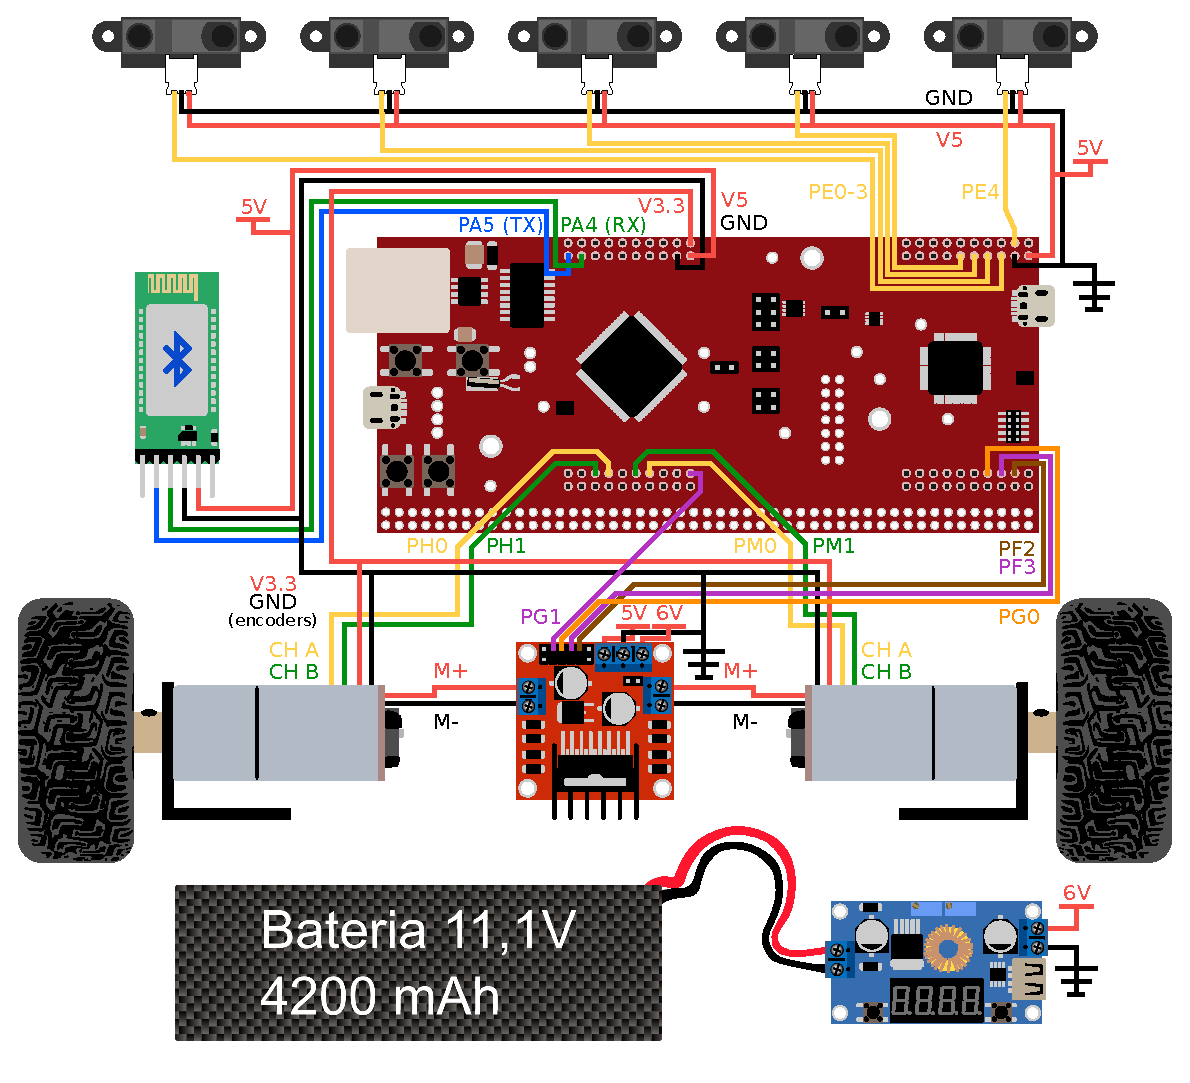
\includegraphics[trim =
		{0cm 0cm 0cm 0cm}, clip, scale=0.8]{Figuras/EsquemaCircuito.eps}};
	\end{tikzpicture}
}
\end{figure}
\end{frame}

\begin{frame}
	\begin{figure}[ht]
	\centering
\resizebox{0.35\linewidth}{!}{
	\begin{tikzpicture}
		\node[anchor=south west,inner sep=0] (image) at (0,0) {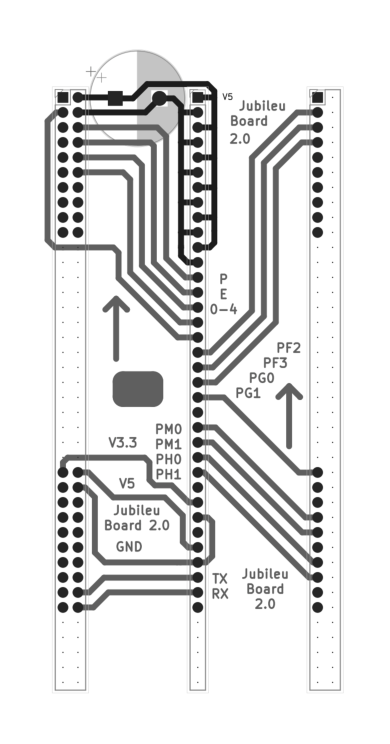
\includegraphics[trim =
		{0cm 0cm 0cm 0cm}, clip,scale=1]{Figuras/JubileuBoard.eps}};
	\end{tikzpicture}	
}
\end{figure}
\end{frame}
	
\begin{frame}
	\frametitle{Comunicação}
	\begin{block}{Interface por Linha de Comando}
		\begin{table}[ht]
\centering
\vspace{0.2 cm}
\resizebox{0.9\linewidth}{!}{
\begin{tabular}{|l|l|}
\hline
\textbf{Comando}       & \textbf{Descrição}                                                                                                                     \\ \hline
SUPERVISOR\_HIBRIDO    & \begin{tabular}[c]{@{}l@{}}Adota o controlador híbrido como a estratégia de \\ navegação utilizada\end{tabular}                        \\ \hline
SUPERVISOR\_FUZZY      & \begin{tabular}[c]{@{}l@{}}Adota o controlador \textit{fuzzy} como a estratégia de\\ navegação utilizada\end{tabular}                  \\ \hline
SETCOORDOBJ(X.XX,Y.YY) & Redefine a coordenada objetivo                                                                                                         \\ \hline
GETSTATE               & \begin{tabular}[c]{@{}l@{}}Utilizado para obter a resposta do estado do robô\\ ($x$, $y$ e $\theta$) a cada iteração, bem como o valor de seus\\ sensores \end{tabular}      \\ \hline
EXIT                   & \begin{tabular}[c]{@{}l@{}}Necessário para solicitar ao robô para que deixe \\ de informar seu estado a cada iteração\end{tabular}     \\ \hline
\end{tabular}
}
\end{table}	
	\end{block}
\end{frame}

%%%%%%%%%%%%%%%%%%%%%%% RESULTADO - SIMULACAO
\begin{frame}
	\frametitle{Resultado para Simulação - Controlador Híbrido}
	\begin{figure}[ht]
		\centering
		% fbox{}
		%\includegraphics[clip, 
%scale=0.058]{Figuras/simulacao_hibrido}
\resizebox{\columnwidth}{!}{
		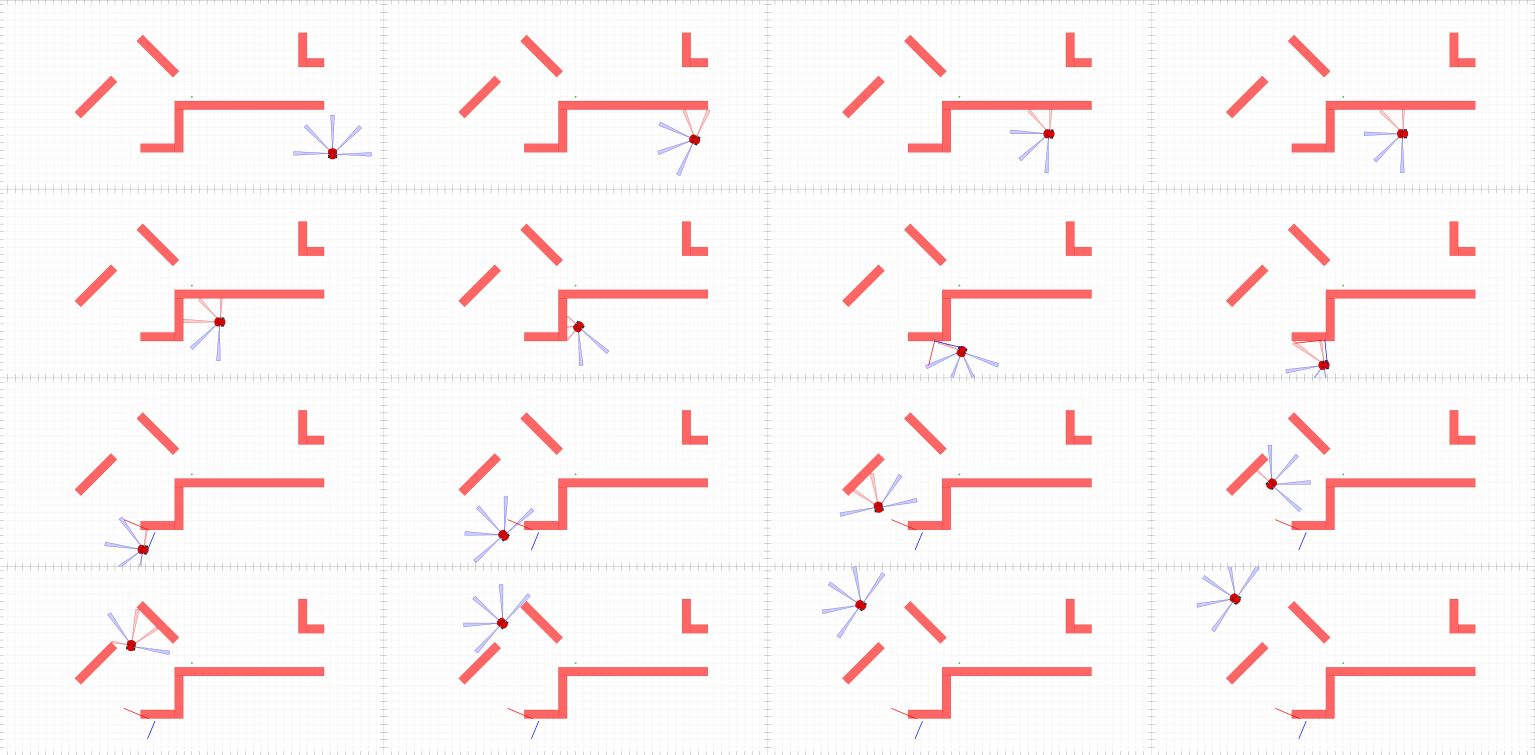
\includegraphics[clip, 
scale=0.29]{Figuras/simulacao_hibridoCompactado}
}
\end{figure}
\end{frame}

\begin{frame}
	\frametitle{Resultado para Simulação - Controlador Fuzzy}
	\begin{figure}[ht]
		\centering
		% fbox{}
		%\includegraphics[clip, 
%scale=0.058]{Figuras/simulacao_fuzzy}
\resizebox{\columnwidth}{!}{
		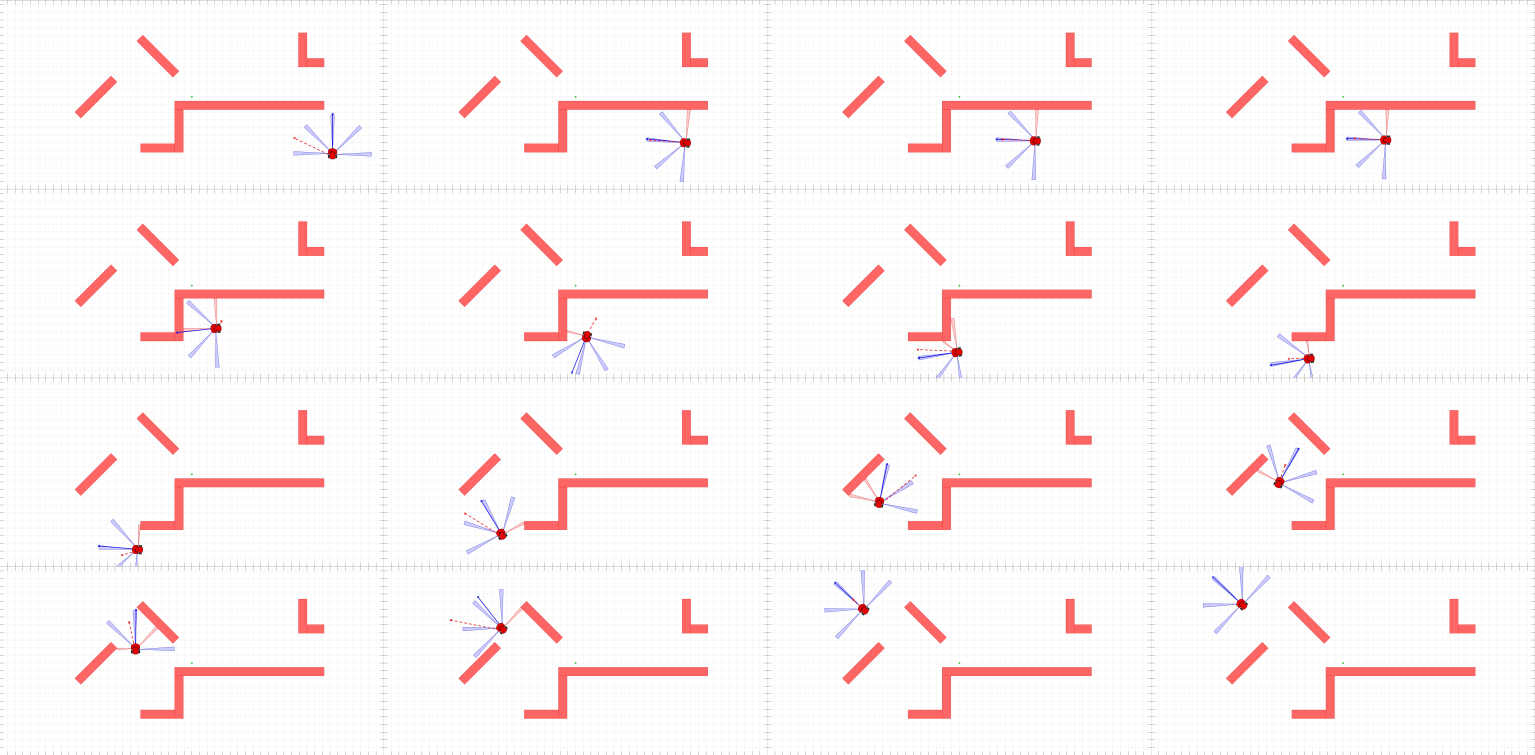
\includegraphics[clip, 
scale=0.29]{Figuras/simulacao_fuzzyCompactado}
}
\end{figure}
\end{frame}

%%%%%%%%%%%%%%%%%%%%%%% RESULTADO - ROBO
\begin{frame}
	\frametitle{Resultado Para o Robô - Controlador Híbrido}
	\begin{figure}[!ht]
\centering
\caption{Resultado do comportamento ``Ir Para Objetivo''}
\label{fig:resultadoImplementadoIPO}
		\centering
		% fbox{}
		%\includegraphics[clip, 
%scale=0.058]{Figuras/ComportamentoIPO}%
		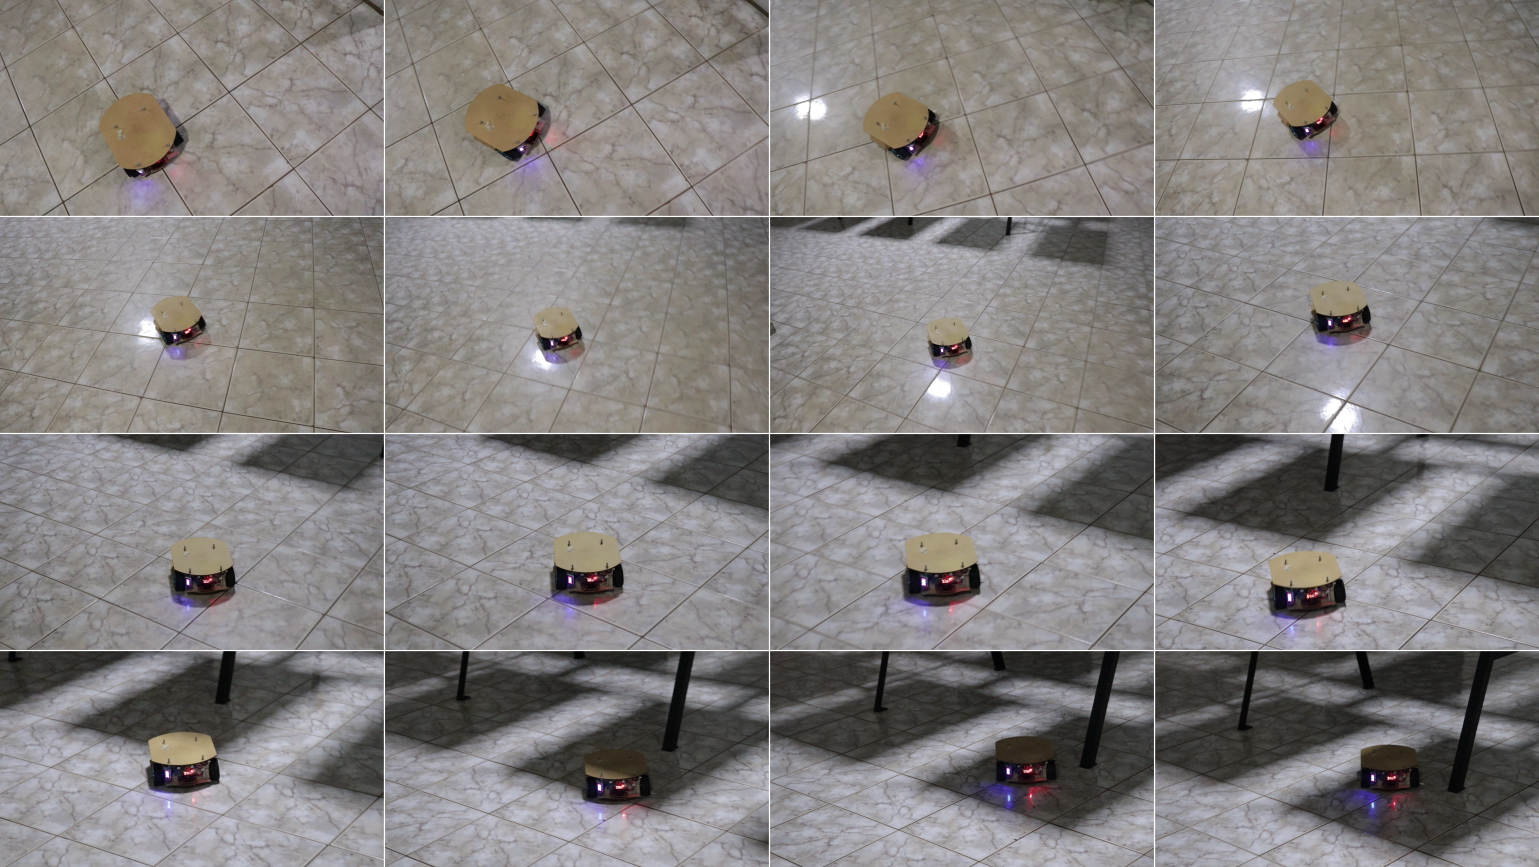
\includegraphics[clip, 
scale=0.29]{Figuras/ComportamentoIPOCompactado}%

	\textbf{Fonte: autoria própria}
\end{figure}
\end{frame}

\begin{frame}
	\frametitle{Resultado Para o Robô - Controlador Híbrido}
	\begin{figure}[!ht]
\centering
\caption{Resultado do comportamento ``Evitar Obstáculo''}
\label{fig:resultadoImplementadoEO}
		\centering
		% fbox{}
		%\includegraphics[clip, 
%scale=0.058]{Figuras/ComportamentoEO}%
		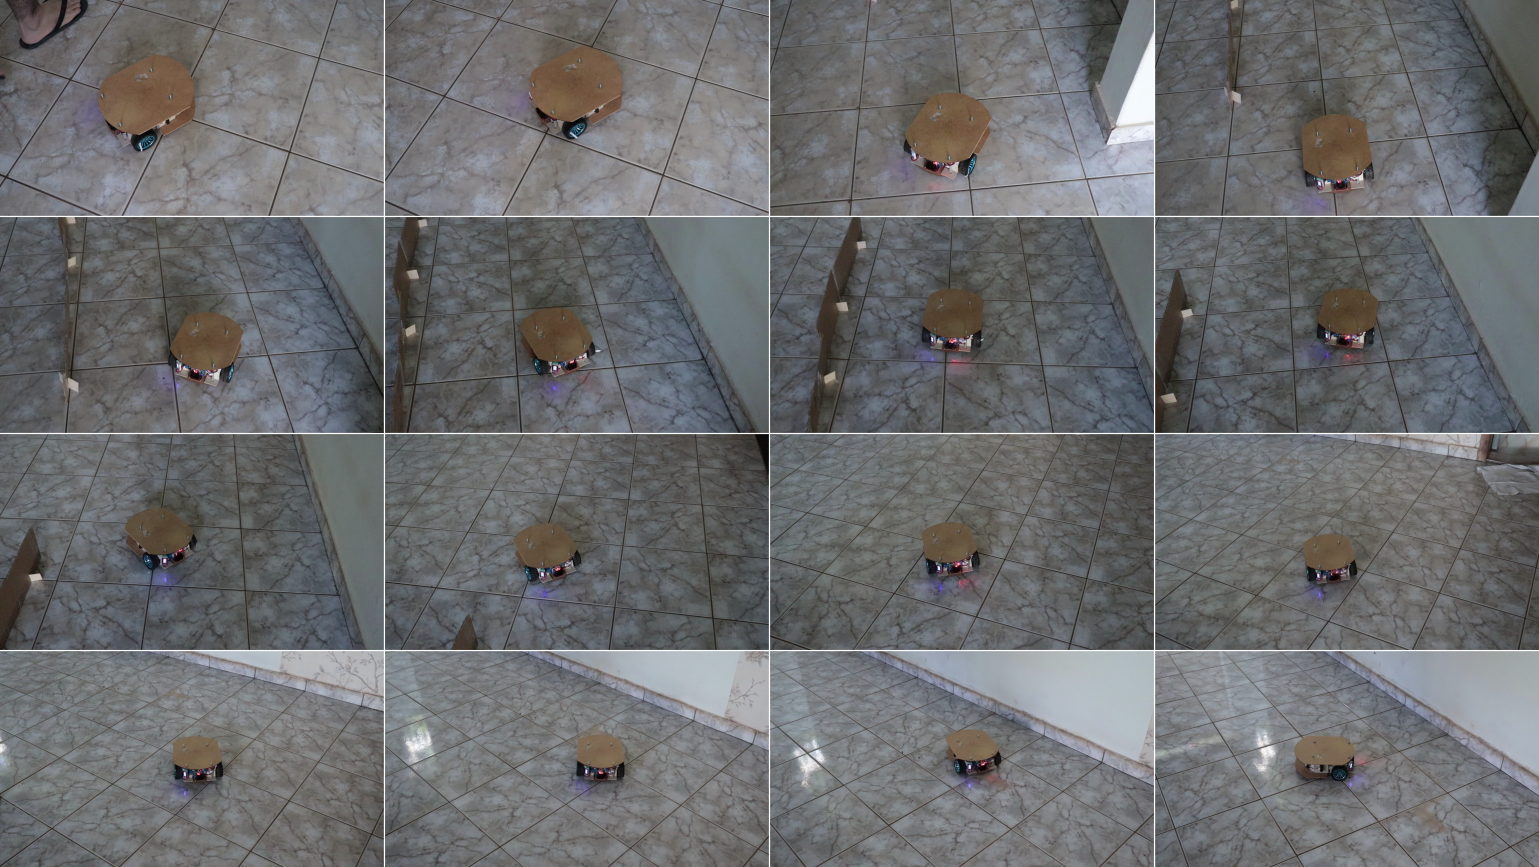
\includegraphics[clip, 
scale=0.29]{Figuras/ComportamentoEOCompactado}%

	\textbf{Fonte: autoria própria}
\end{figure}
\end{frame}

\begin{frame}
	\frametitle{Resultado Para o Robô - Controlador Híbrido}
	\begin{figure}[!ht]
		\centering
		% fbox{}
		%\includegraphics[clip, 
%scale=0.058]{Figuras/ComportamentoIPO_E_EO}%
\resizebox{\columnwidth}{!}{
		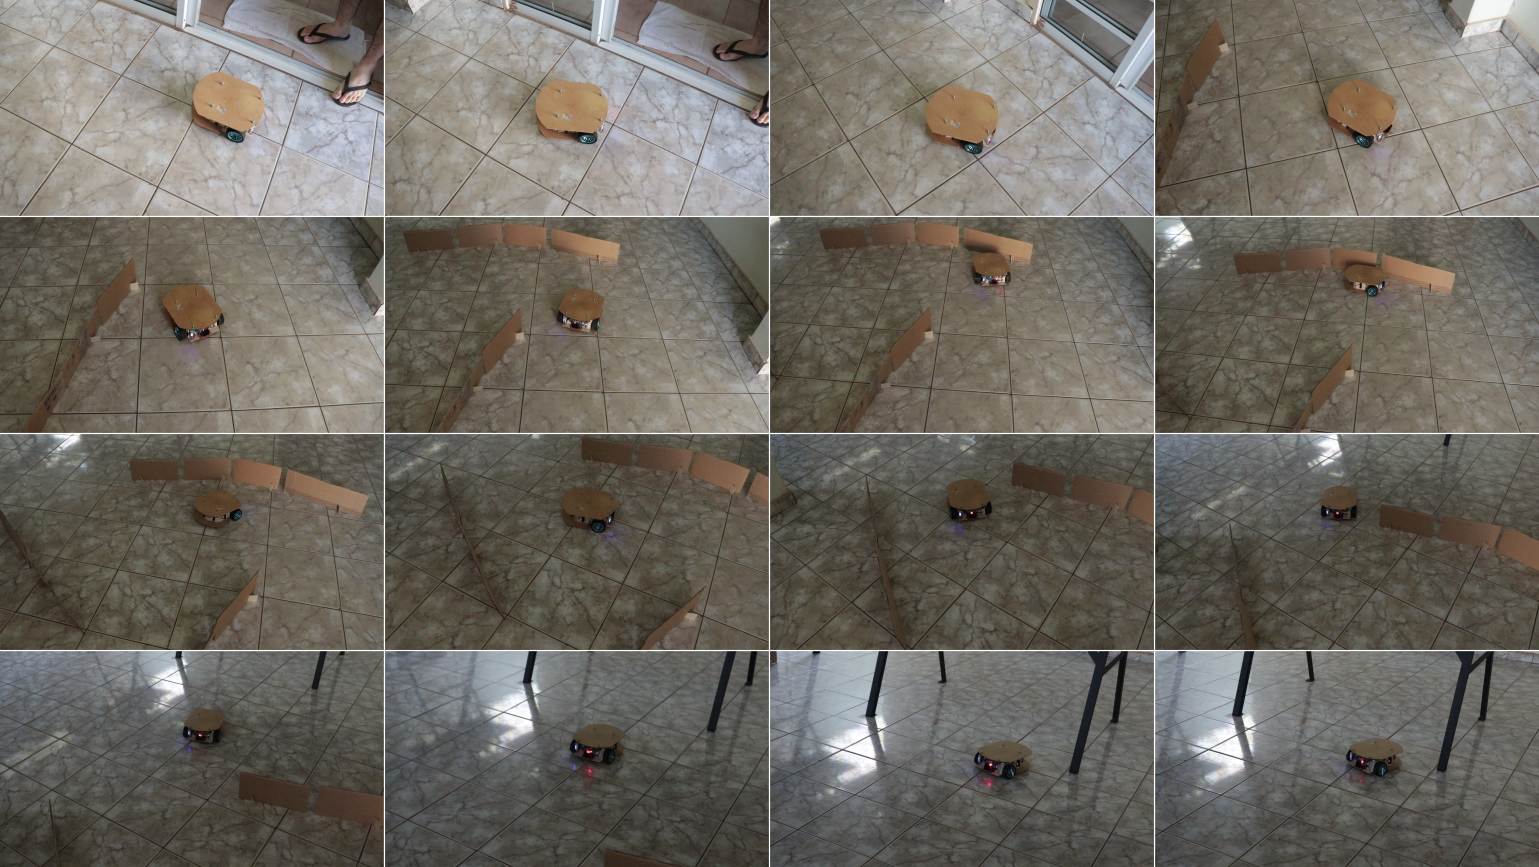
\includegraphics[clip, 
scale=0.29]{Figuras/ComportamentoIPO_E_EOCompactado}%
}
\end{figure}
\end{frame}

\begin{frame}
	\frametitle{Resultado Para o Robô - Controlador Híbrido}
	\begin{figure}[!ht]
\centering
\caption{Resultado do comportamento ``Seguir Parede''}
\label{fig:resultadoImplementadoSP}
		\centering
		% fbox{}
		%\includegraphics[clip, 
%scale=0.058]{Figuras/ComportamentoSP}%
		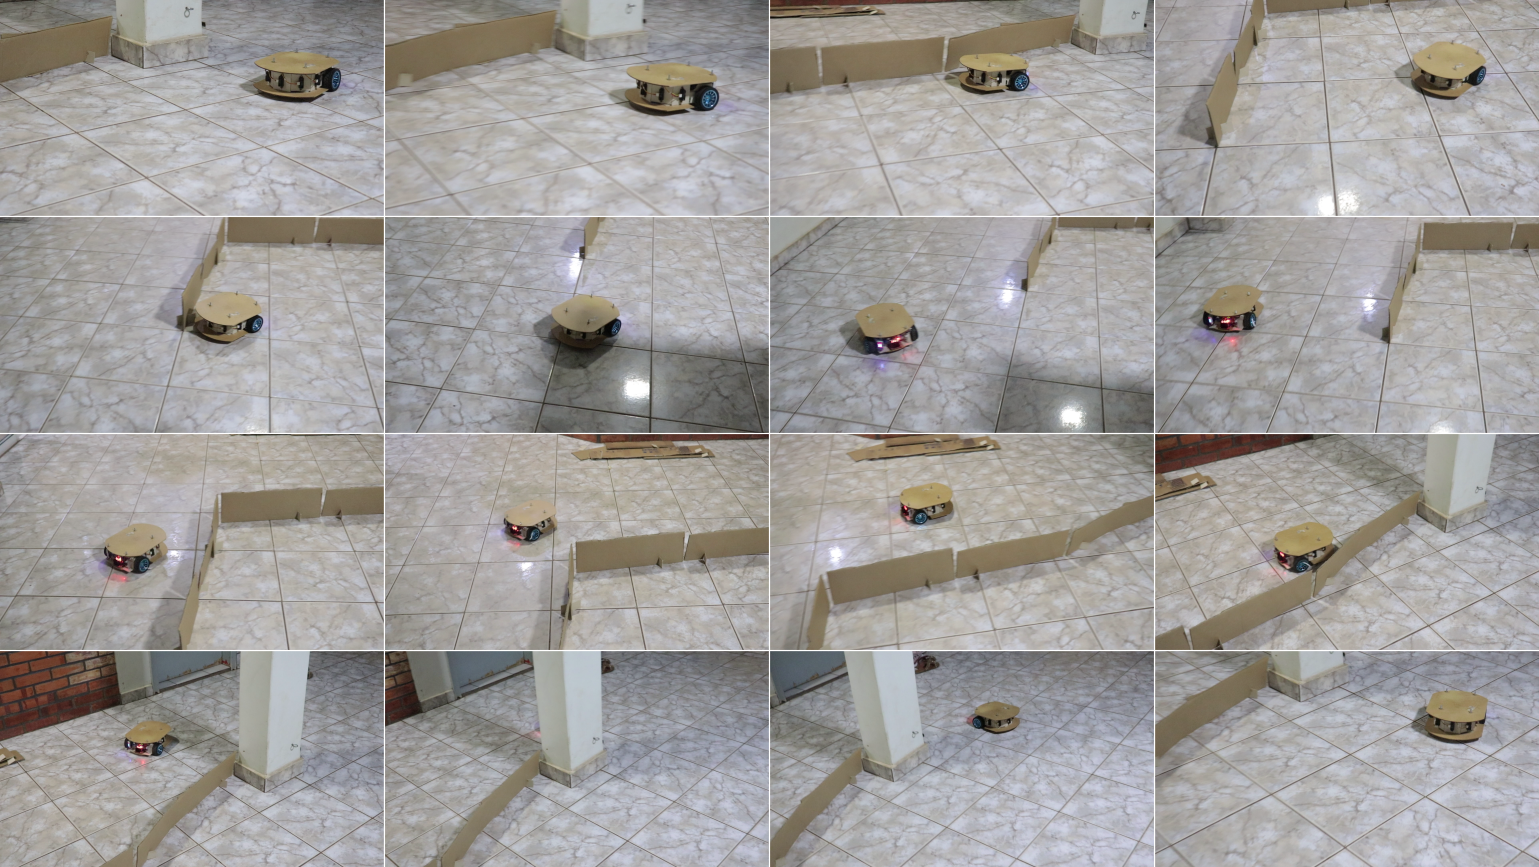
\includegraphics[clip, 
scale=0.29]{Figuras/ComportamentoSPCompactado}%

	\textbf{Fonte: autoria própria}
\end{figure}
\end{frame}

\begin{frame}
	\frametitle{Resultado Para o Robô - Controlador Híbrido}
	\begin{figure}[ht]
\centering
\caption{Resultado implementado para o controlador híbrido}
\label{fig:resultadoImplementadoHibrido}
		\centering
		% fbox{}
		%\includegraphics[clip, 
%scale=0.058]{Figuras/hibrido}%
		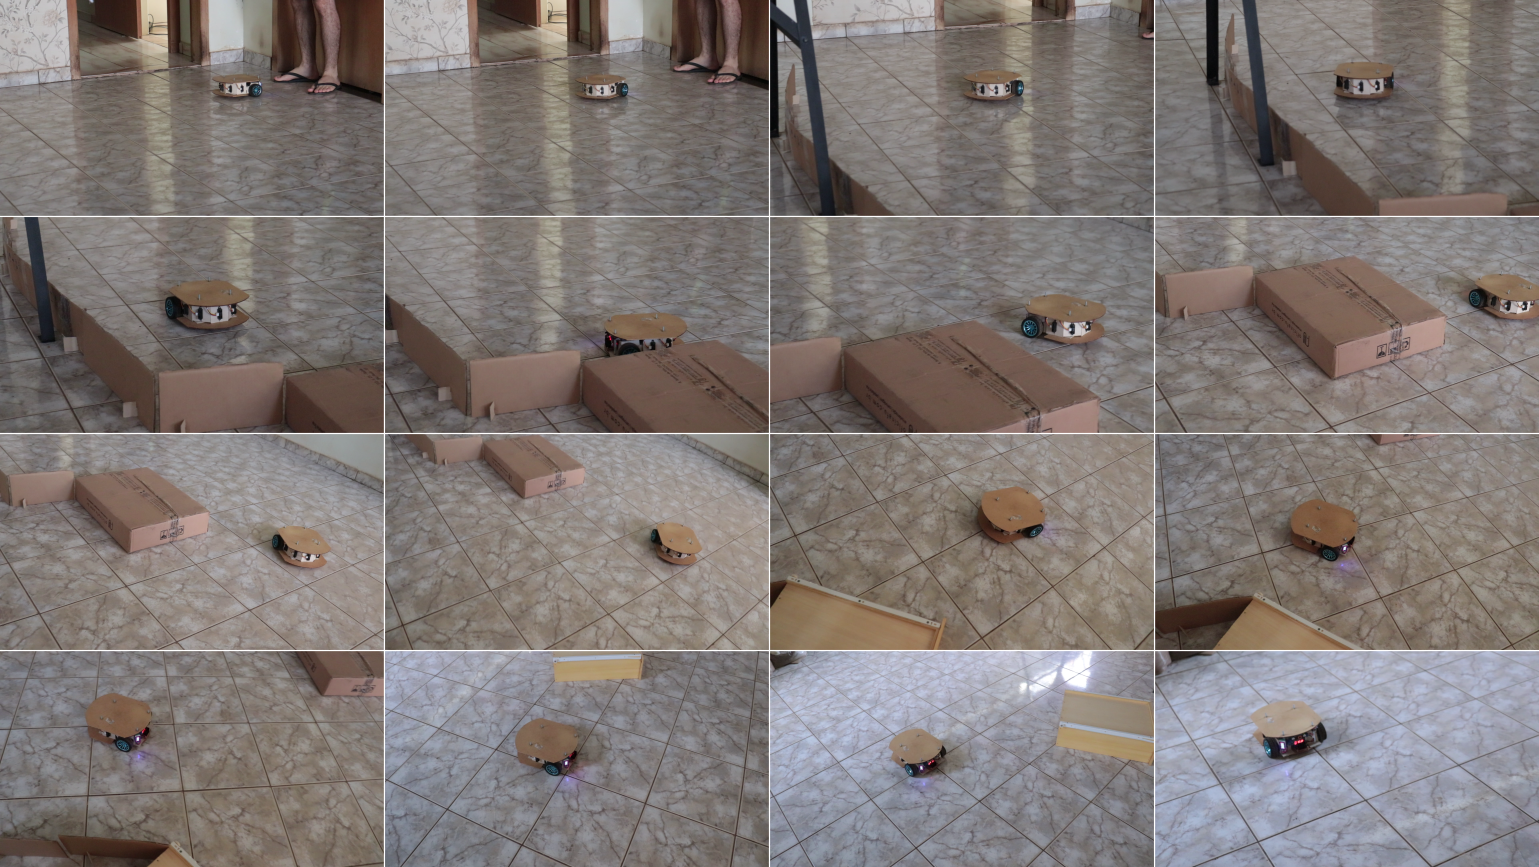
\includegraphics[clip, 
scale=0.29]{Figuras/hibridoCompactado}%

	\textbf{Fonte: autoria própria}
\end{figure}
\end{frame}

\begin{frame}
	\frametitle{Resultado Para o Robô - Controlador Fuzzy}
	\begin{figure}[ht]
\centering
\caption{Resultado implementado para o controlador \textit{fuzzy}}
\label{fig:resultadoImplementadoFuzzy}
		\centering
		% fbox{}
		%\includegraphics[clip, 
%scale=0.058]{Figuras/fuzzy}
		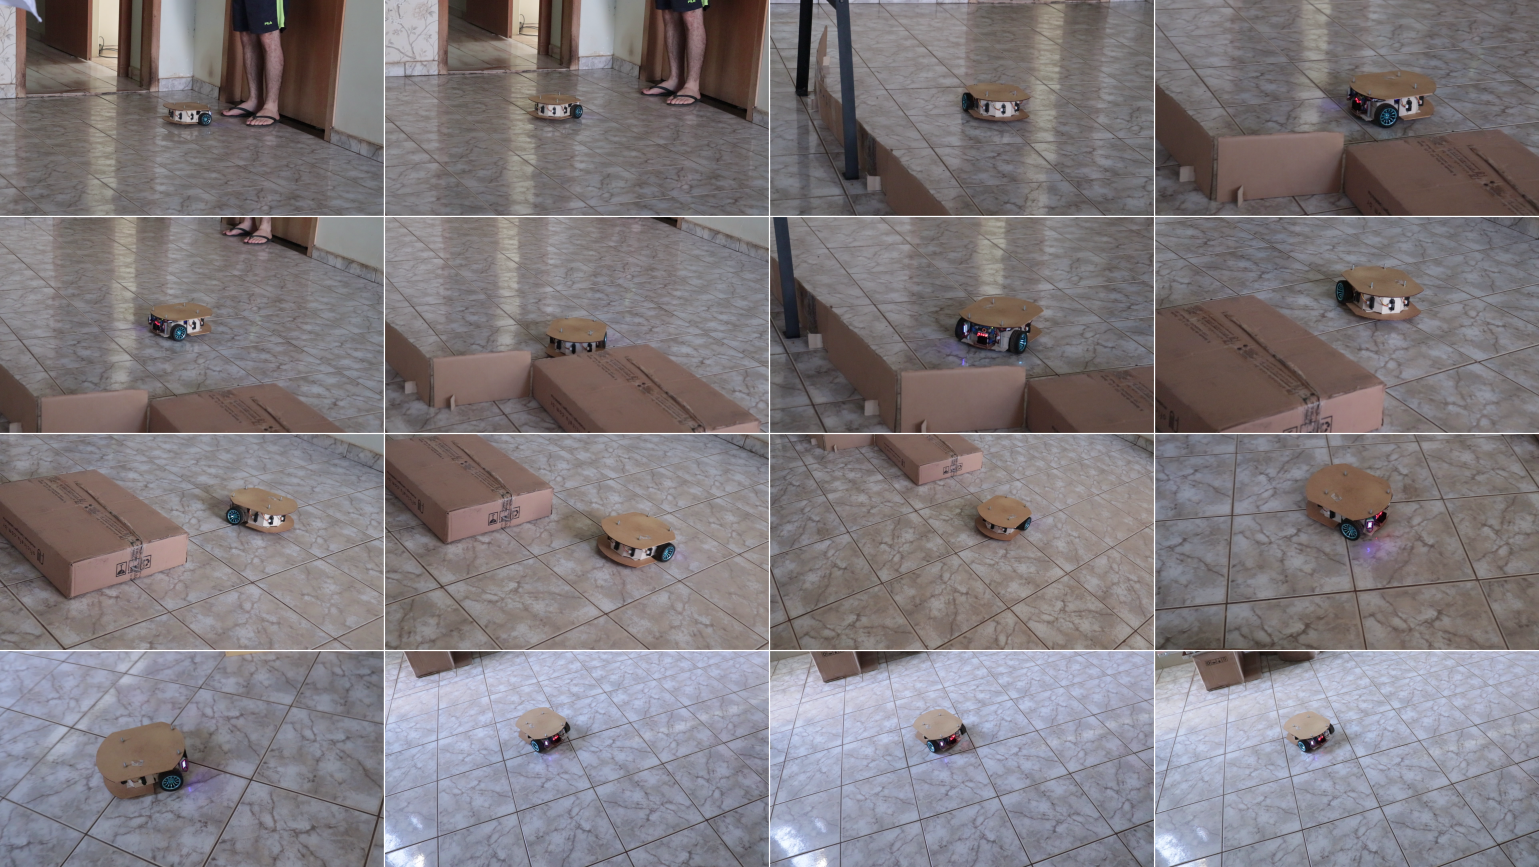
\includegraphics[clip, 
scale=0.29]{Figuras/fuzzyCompactado}

	\textbf{Fonte: autoria própria}
\end{figure}
\end{frame}

	
	% Consideracoes Finais
	\subsection{Considerações Finais}
\begin{frame}
	\frametitle{Considerações Finais}
	
	\begin{block}{}
		\begin{itemize}
		  \item Autonomia em arquiteturas não deliberativas.
		  \item Estimativa de estado.
		  \item Comparação qualitativa.
		\end{itemize}
	\end{block}
\end{frame}
	
	% Agradecimentos
	\subsection{Agradecimentos}
\begin{frame}
	%\frametitle{Obrigado pela presença!}
	\titlepage
\end{frame}

\end{document}